\documentclass[11pt,a4paper]{article}
\usepackage[latin1]{inputenc}
\usepackage{amsmath}
\usepackage{pdflscape}
\usepackage{rotating}
\usepackage{amsfonts}
\usepackage{tabu}
\usepackage{cite}

\numberwithin{equation}{subsection}
\usepackage[titletoc]{appendix}
\usepackage{amssymb}
\usepackage{graphicx}
\usepackage{tabularx}
\usepackage{caption}
\usepackage{multirow}
\usepackage{setspace}
\usepackage{fancyhdr}
\usepackage[export]{adjustbox}
%\usepackage{floatrow}
%\usepackage[singlelinecheck=off]{caption}
\DeclareRobustCommand\nocite[1]{%
	{\def\cite##1{\ignorespaces}#1}}
\newcommand\nocitecaption[1]{\caption[\nocite{#1}]{#1}}

% Set folder for images
\graphicspath{ {Figures_and_Images/} }

% Set Margins
\usepackage{geometry}
\geometry{, total={145mm,247mm}, left = 40mm, top = 25mm}

% Set Font
\usepackage{pslatex} %Times font

% Set up Left Align Table Caption
 \captionsetup[table]{
 	labelsep = newline, 
 	name = Table, 
 	justification=justified,
 	singlelinecheck=false,%%%%%%% a single line is centered by default
 	labelsep=colon,%%%%%%
 	skip = \bigskipamount}
 
  \captionsetup[figure]{
  	labelsep = newline, 
  	name = Figure, 
  	justification=justified,
  	singlelinecheck=true,%%%%%%% a single line is centered by default
  	labelsep=colon,%%%%%%
  	skip = \bigskipamount}


%--------------------------------------------------------------
%	TITLE PAGE
%--------------------------------------------------------------
\thispagestyle{empty}

\newcommand*{\titleGP}{\begingroup % Create the command for including the title page in the document
	\centering % Center all text
	\vspace*{\baselineskip} % White space at the top of the page
	
	
	{\Large JAMES COOK UNIVERSITY\\ [0.3\baselineskip] } % Title
	
	{\Huge COLLEGE OF SCIENCE \&{} ENGINEERING\\ [0.3\baselineskip] } % Title
	
	\vspace*{7\baselineskip} % Whitespace between location/year and editors
	
	{\Huge EG4011\\ Civil Engineering\\ [0.3\baselineskip] } % Title
	
	\vspace*{6\baselineskip} % Whitespace between location/year and editors
	
	{\Huge \bf{A STUDY OF THE EFFECTS OF NOTCHING ON RECTANGULAR AND ROUND TIMBER GIRDERS}\\ [0.3\baselineskip] } % Title
	
	\vspace*{2\baselineskip} % Whitespace between location/year and editors
	
	{\LARGE LARA MULLAMPHY\par} % Editor list

	
	\vfill % Whitespace between editor names and publisher logo
	
	
		\scshape % Small caps
		Proposal submitted to the School of Engineering and Physical Sciences in partial fulfilment of the requirements for the degree of \\
		{\Large Bachelor of Engineering\\ (Civil Engineering)} % Tagline(s) or further description
		\\[\baselineskip] % Tagline(s) or further description
		29 April 2016\par % Location and year
	
	\endgroup}

%--------------------------------------------------------------

\begin{document}

%------------------------- Title Page -------------------------
	\titleGP % This command includes the title page

	% Set Line Spacing to 1.5
	\setstretch{1.5}
	
	\pagestyle{fancy}
%	\thispagestyle{empty}
	\fancyhead{}
	\fancyfoot{}
	\renewcommand{\headrulewidth}{0pt}
	\fancyfoot[R]{\thepage}
	\pagenumbering{roman}
	\pagebreak
%-------------------- Statement of Access -----------------------
% See Thesis manual

%-------------------- Declaration of Sources -------------------

% See Thesis manual

%-------------------- Table of Contents -------------------	 
	\tableofcontents
	\vspace*{\baselineskip}
	\vspace*{\baselineskip}
	
	\pagebreak

	\nocite\listoffigures 
	\addcontentsline{toc}{section}{List of Figures}
	\listoftables
	\addcontentsline{toc}{section}{List of Tables}
	\pagebreak
	
%---------------------- Introduction --------------------------
	\section{Introduction}
	
	\pagenumbering{arabic}
	\setcounter{page}{1}
	% State the general topic

	
	\noindent
	Timber has been a dominant material in engineering and construction for centuries and continues to be a major material used in housing, floors and furniture. Timber was also the first material used to construct bridges and, although it is slowly being replaced by alternative building materials, there are currently around 20,000 timber road bridges still currently in use within Australia. Many of the bridges still in use are utilised by rail \cite{wilkinson_capacity_2008} which is subject to significant load and hence the maintenance and strengthening of these bridges is of major importance. 
    
    \vspace*{\baselineskip}
    
    \noindent
    Over the past few decades there has been a major decrease in the use of timber for the construction of bridges. This is predominately due to the inherent properties of timber which expose it to environmental problems such as weathering, rotting and insect infestation. These conditions make the bridge expensive to maintain and significantly limits the lifespan of the structure.  Hence the majority of bridges now being constructed in Queensland utilise steel and concrete to minimize the impact of any environmental damage. However, many timber bridges throughout Queensland still remain in use and hence require regular maintenance and strengthening to withstand growing load demands and remain stable until they are eventually replaced. As the complete replacement of bridges is expensive, the alternative of strengthening the structure appears to be the more feasible option. One of the primary sections of timber bridges which require strengthening are the notches in the timber beams. These sections are particularly prone to cracking and need to be studied in order to find a suitable method for strengthening these regions.
	
	\vspace*{\baselineskip}
	
	\noindent
     Notching is when a section from a member is cut out to ease insertion and act as seating for timber girders over piers or abutments. This is common practice in the construction of timber bridges and places increased risk of failure to the structure at the position of the notches.This increased risk occurs due the section loss from notching exposing the timber to the risk of cracking and potential failure. As notches reduce beam capacities, the need to strengthen this area is of high importance. Currently there is little information on notching design surrounding circular members or evaluating capacities of a notched round member. This is of significant importance in the construction of timber bridges as most members currently used in bridges are round. A study of the literature has revealed that there have been very few studies carried out on the strengthening of these notches in circular section beams. Hence there remains a strong need for further investigation, with a particular emphasis for the strengthening of notches in circular members used in the construction of timber bridges. 
	
	\vspace*{\baselineskip}
	
	\noindent
    The proposed research will provide further understanding into the effects of notches and notch angles on round timber members. Current notch design methods will be investigated and compared to determine which method obtains the most accurate results. As many bridges are currently suffering issues caused by notching, the ability to understand the effects of notching will assist in a further understanding of how to design and possibly strengthen them. By establishing an effective method of notch design, 
    %increase their lifespan and delay the need for total replacement will be of significant importance to reducing the overall costs associated with timber bridges.  
	
	
	\subsection{Objectives}
	The aim of this research was to determine the structural behaviour of rectangular and circular section timber girders with different notched angles. The main objectives were to:\par 
	
	\begin{enumerate}
		\item Determine the effects of different notch types on the flexural and shear capacity of rectangular and circular timber beams
		\item Validate existing design equations for notched timber girders
		\item Develop a finite element analysis model to simulate the behaviour of both strengthened and un-strengthened notched timber girders.
	\end{enumerate}
	
	\subsection{Scope}
	\noindent
	The overall scope of this research was to determine the effects of notching on rectangular and circular section members, and to determine which methods of notch design yield the most accurate results. This was achieved through small-scale experiments where notch angles were altered on both section types. 
	
	\pagebreak
	
	\section{Literature Review}
	
	\subsection{Timber Bridges}
	Timber has been used in the construction of bridges for thousands of years \cite{ritter_timber_1990} and remained the preferred construction material until the middle of the 20th century when it was eventually replaced by the introduction of steel and concrete \cite{ritter_timber_1990,_timber_2005} . Timber had remained the dominant building material because of its strength and light weight. Timber also has energy- absorbing properties, making it capable of handling short term overloads without harmful effects, making it an excellent material for bridge construction. Large timber members also have good fire resistance qualities, are relatively durable and have the ability to withstand de-icing effects. Overall the construction of timber bridges is very cost effective as timber is a relatively cheap and renewable resource and installation can usually be carried out without the need of heavy machinery, significantly reducing the labour required \cite{ritter_timber_1990}. Although timber bridges are relatively cost effective to build, susceptibility to weather and insects make them expensive to maintain.
	
	\vspace*{\baselineskip}
	
	\noindent
	Ongoing repairs for the timber structure can be labour intensive and expensive, hence preventative maintenance is important in cutting costs and prolonging the life of the bridge. To prevent deterioration, the timber can be chemically treated against damage to weathering from sunlight exposure and moisture. This is a major benefit as there is little to no maintenance or painting required for wood treated with preservatives \cite{ritter_timber_1990}. Furthermore, the wood can be treated to prevent pest infestation \cite{_timber_2005,ritter_timber_1990} which can cause major damage to any timber structure. The commonplace use of chemical treatment to preserve timber bridges has almost certainly added decades to the life of the bridge. However, when significant damage has already occurred, strengthening may be the only feasible option to prevent further damage and eventual failure of the bridge.
	
	\vspace*{\baselineskip}
	
	\noindent
	The availability of suitable timber is now a major concern for existing timber bridges which require substantial maintenance throughout their structural life \cite{_timber_2005}. The ability to source large sections of wood and sawn timber is becoming increasingly more difficult as the amount of timber suitable for harvesting decreases over time. The drive for forest preservation has also increased, heavily reducing the amount of suitable timber needed for bridge construction and maintenance \cite{_timber_2005,ritter_timber_1990}. This is another strong reason for strengthening current structures as the raw materials required for repair or replacement of timber bridges are costly and difficult to source.
	
	\subsubsection{Wood Types}
	There are two classes of timber; hardwood and softwood. The two types of wood can initially be distinguished by their leaves as hardwood trees have broad leaves and softwood trees have sharp needle like foliage \cite{dunningham_review_2015}. 
	
	\vspace*{\baselineskip}
	
	\noindent
	The major difference between hardwood and softwood is their cell structures \cite{stalnaker_structural_2013}. Hardwood contains mainly fibres, vessels/pores and parenchymas whereas softwoods contain tracheids (early- and latewood), resin canals and parenchymas \cite{cresswell_product_2004}.
	
	\vspace*{\baselineskip}
	
	\noindent
	It can be seen in Figure \ref{fig:Wood} that the cell structure of hardwood is substantially more complex than softwood \cite{mohanty_natural_2005}. The cell structure of softwood has a organised arrangement, whereas the cell arrangement of hard wood appears more random. A common misconception is that hardwood is hard in comparison to softwood, however this is not necessarily the case \cite{pipinato_innovative_2015,marshall_black_2005}. To determine whether to use softwood or hardwood, the major deciding factor is based on the intended purpose of the wood (i.e. whether it is to be in tension or compression).
	
		\begin{figure}[h]
			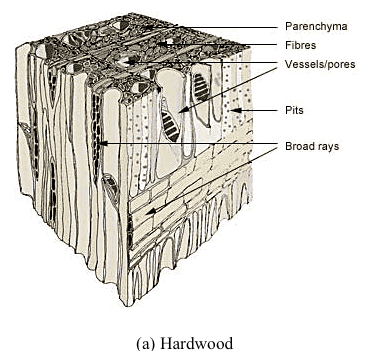
\includegraphics[scale=0.6]{Hardwoods}
			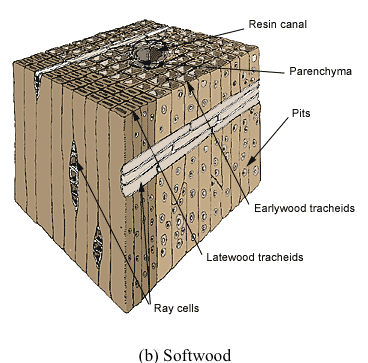
\includegraphics[scale=0.6]{Softwoods}	
			\caption{Wood Cell Structures \cite{_softwood_2016}}
			\label{fig:Wood}
		\end{figure}
	
	
	\noindent
	Table \ref{tab:Aspect} compares the aspect ratio of hardwood and softwood; these differ depending on the exact wood used and their particle/fibre size. From this it can be seen that generally hardwoods have a higher aspect ratio which implies they have better bending abilities, and thus are superior in sustaining tensile loads \cite{klyosov_wood-plastic_2007}. 
	
	\pagebreak
	\begin{center}
		\captionof{table}{Wood Cell Structures \cite{_softwood_2016}}
		\label{tab:Aspect}
		\begin{tabular}{c c c} 
			\hline
			\multirow{2}{*}{Particle size Range} & \multicolumn{2}{c}{Aspect Ratio} \\
			\cline{2-3}
			
			& Hardwoods & Softwoods \\ [0.5ex] 
			\hline
			20 mesh $(850\mu m - 0.85mm)$ & 4.6 & 3.5 \\ [0.5ex]
			
			40 mesh $(425\mu m - 0.425mm)$ & 4.4 & 3.4 \\ [0.5ex]
			
			60 mesh $(250\mu m - 0.25mm)$ & 4.4 & 4.2 \\ [0.5ex]
			
			800 mesh $(180\mu m - 0.18mm)$ & 4.2 & 4.5 \\ [0.5ex]
			
			\hline
			
		\end{tabular}
	\end{center}
	
	\vspace*{\baselineskip}
	
	\noindent
	More commonly used in timber bridge structures in Australia is hardwood due to its abundance at the time of construction\cite{rta_timber_2000}, as well its combination of high strength, durability, light-weight and most importantly flexural properties \cite{klyosov_wood-plastic_2007}. Commonly used woods in Queensland bridges are spotted gum, tally-wood and swamp mahogany. Spotted gum is strong, light-weight, tough, elastic and durable, and is particularly well-performing when in tension. Tally-wood is strong, durable and very tough; it withstands underground and aqueous conditions and is used mainly in decking and posts. Swamp mahogany is elastic, strong, tough and durable, which also sustains well in underground and aqueous conditions; it is predominately used in piles \cite{_queensland_1899}.
	
	\subsubsection{Common Defects and Failures}
    There are four major defects that are commonly occurring in timber bridges; weathering, rot- ting, cracking and termite infestation. These defects severely reduce the lifespan of a timber bridge and will all eventually lead to member failure.

    \vspace*{\baselineskip}
    
    \noindent
    \textbf{Weathering and Rotting}

	\noindent
	Weathering and rotting occur in timber members due to exposure to a combination of wind, wetting, drying and UV radiation \cite{_timber_2005,_section_2008}. The appearance of the weathering damage depends on the elements the timber is exposed to. Exposure to high wind speeds can cause dints/abrasions from small pebbles or embedded sand particles \cite{harrowfield_analysis_2006}, whereas exposure to a combination of running water and sun light can cause a ripple effect, as shown on a rail bridge longitudinal girder in the Figure \ref{fig:Weather}.
	
\begin{figure}[h]
	\begin{center}
		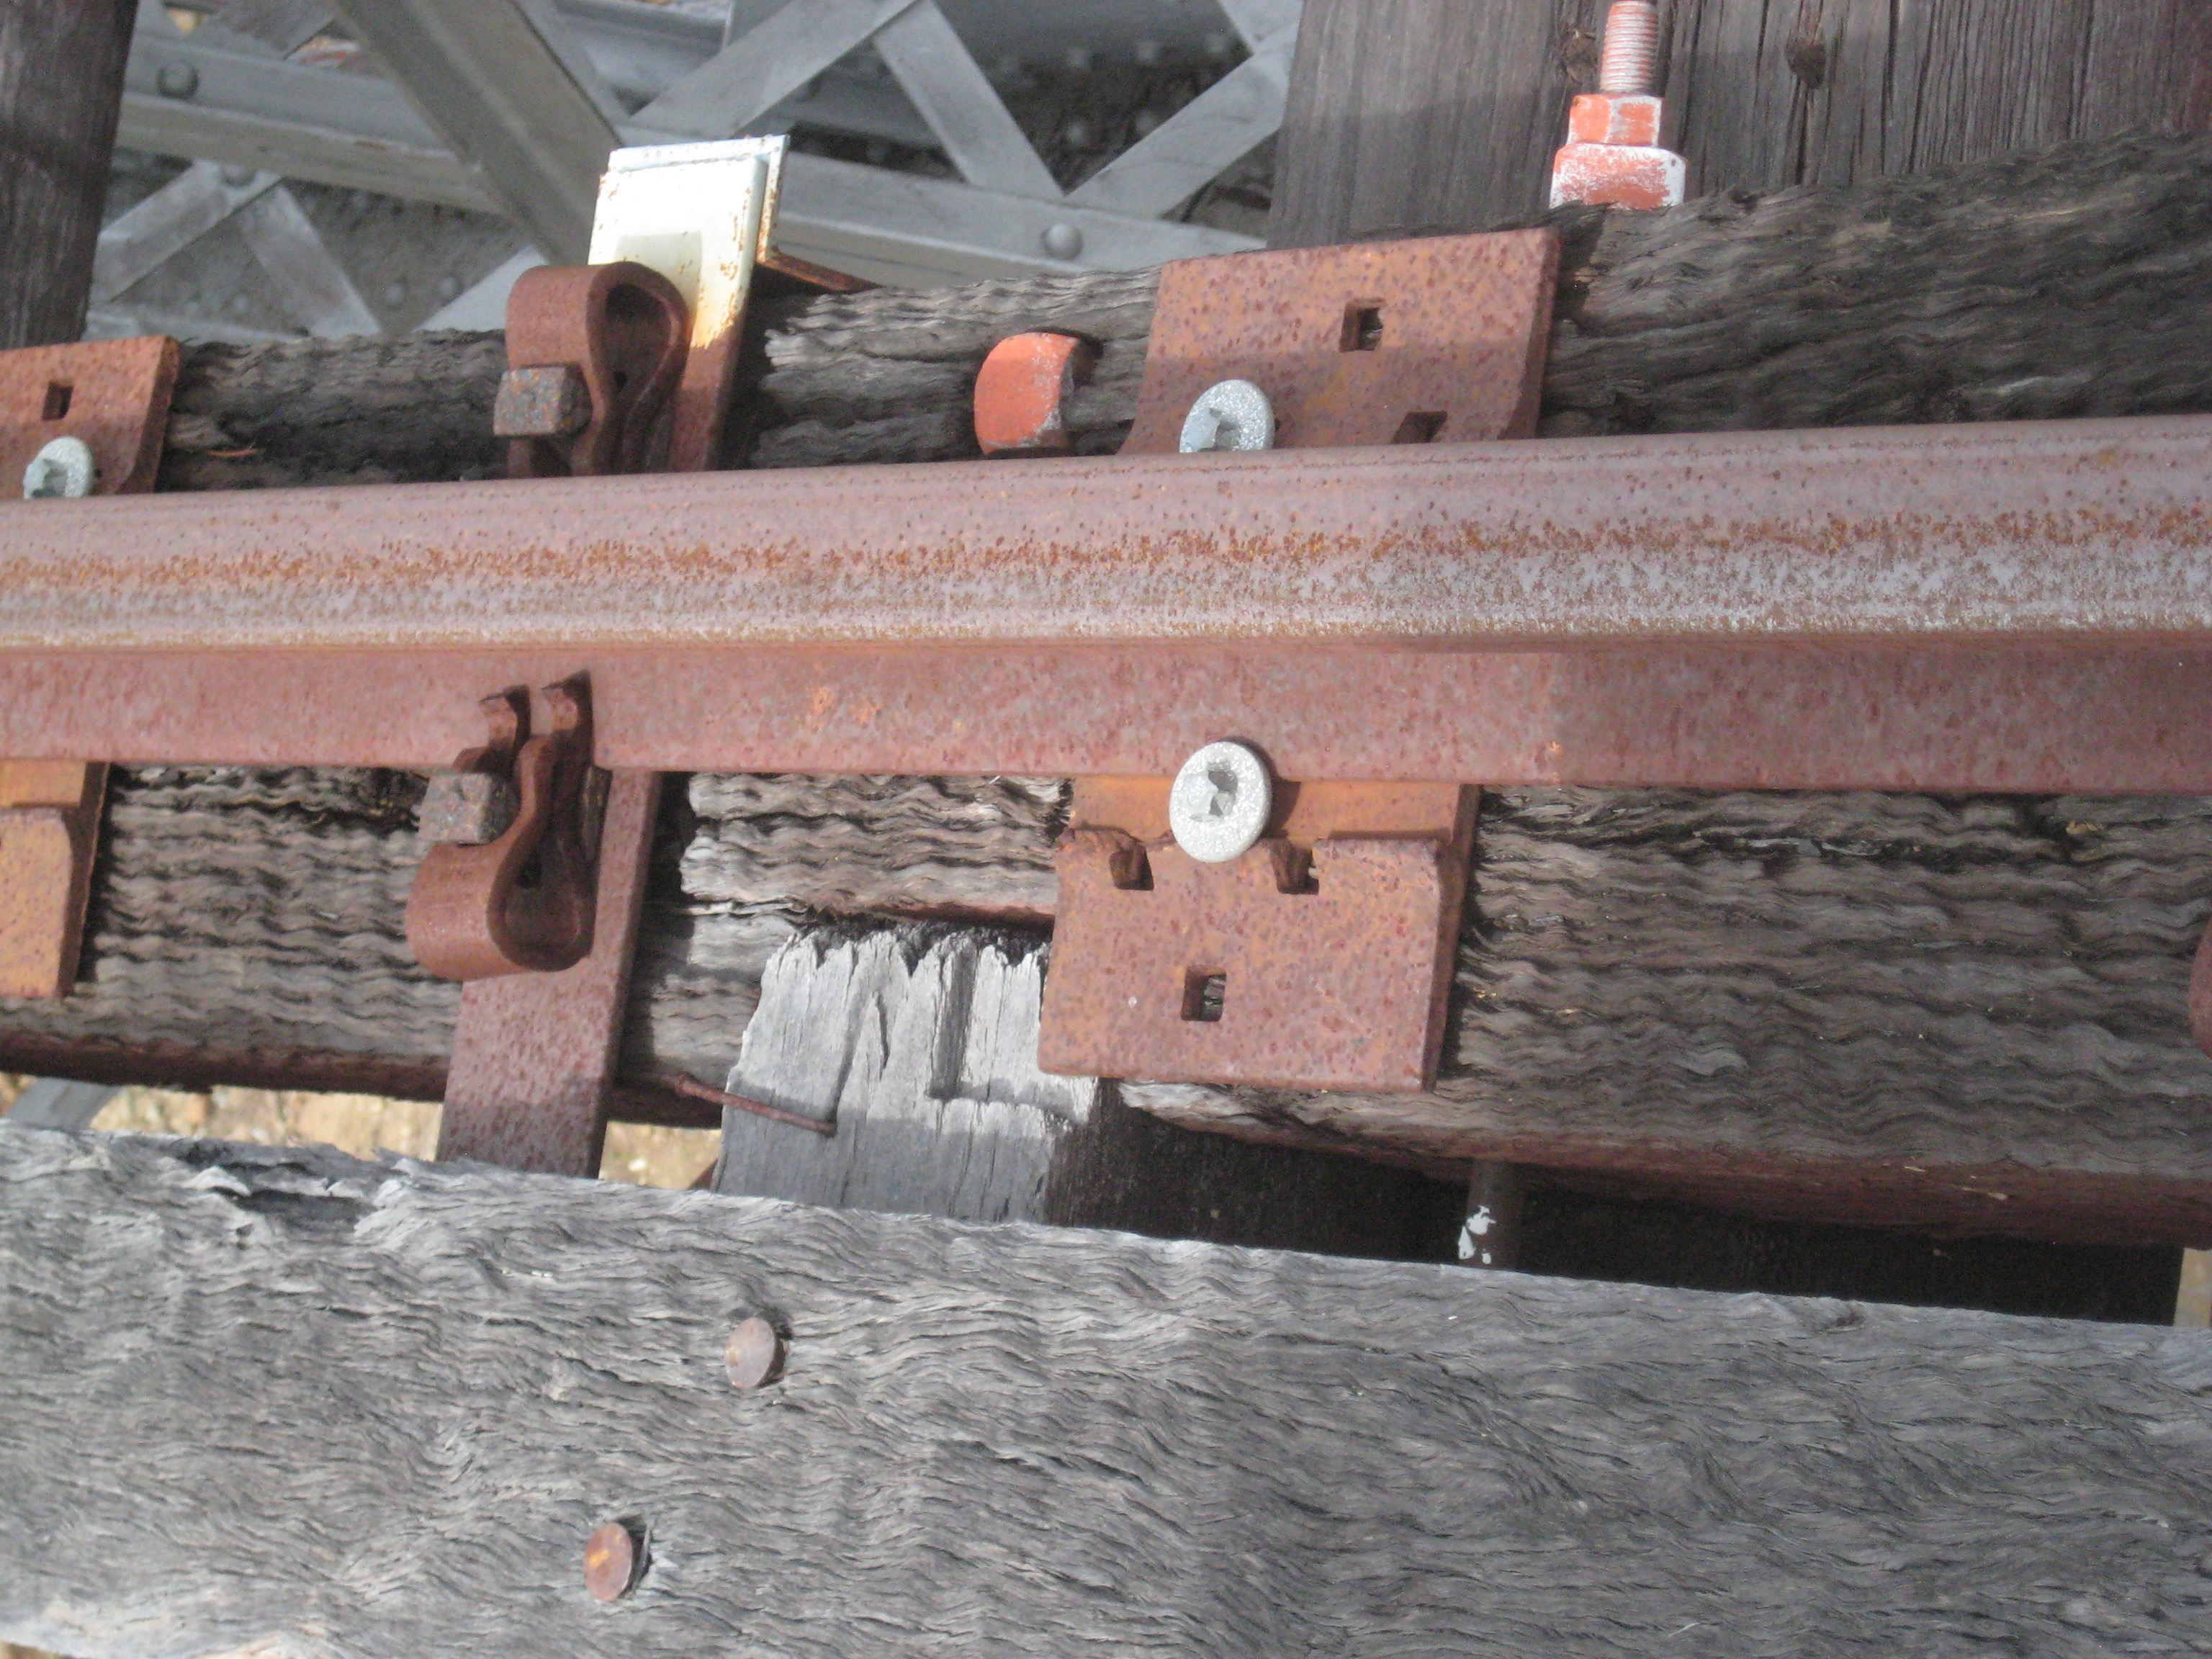
\includegraphics[scale=0.07]{Weathering}
	\end{center}
	\caption{Weathering}
	\label{fig:Weather}
\end{figure}
	\pagebreak
	
	 \noindent
	 Rotting occurs in areas where moisture is allowed to penetrate the wood and can lead to core rotting as shown in Figure \ref{fig:Rot} which severely reduces the strength of the member. The most vulnerable areas for rotting occur at bolt holes and cut sections (i.e. notches) where moisture can easily penetrate the timber \cite{_timber_2005,white_bridge_1992}. 
	 \vspace*{\baselineskip}
	 	\begin{figure}[h]
	 		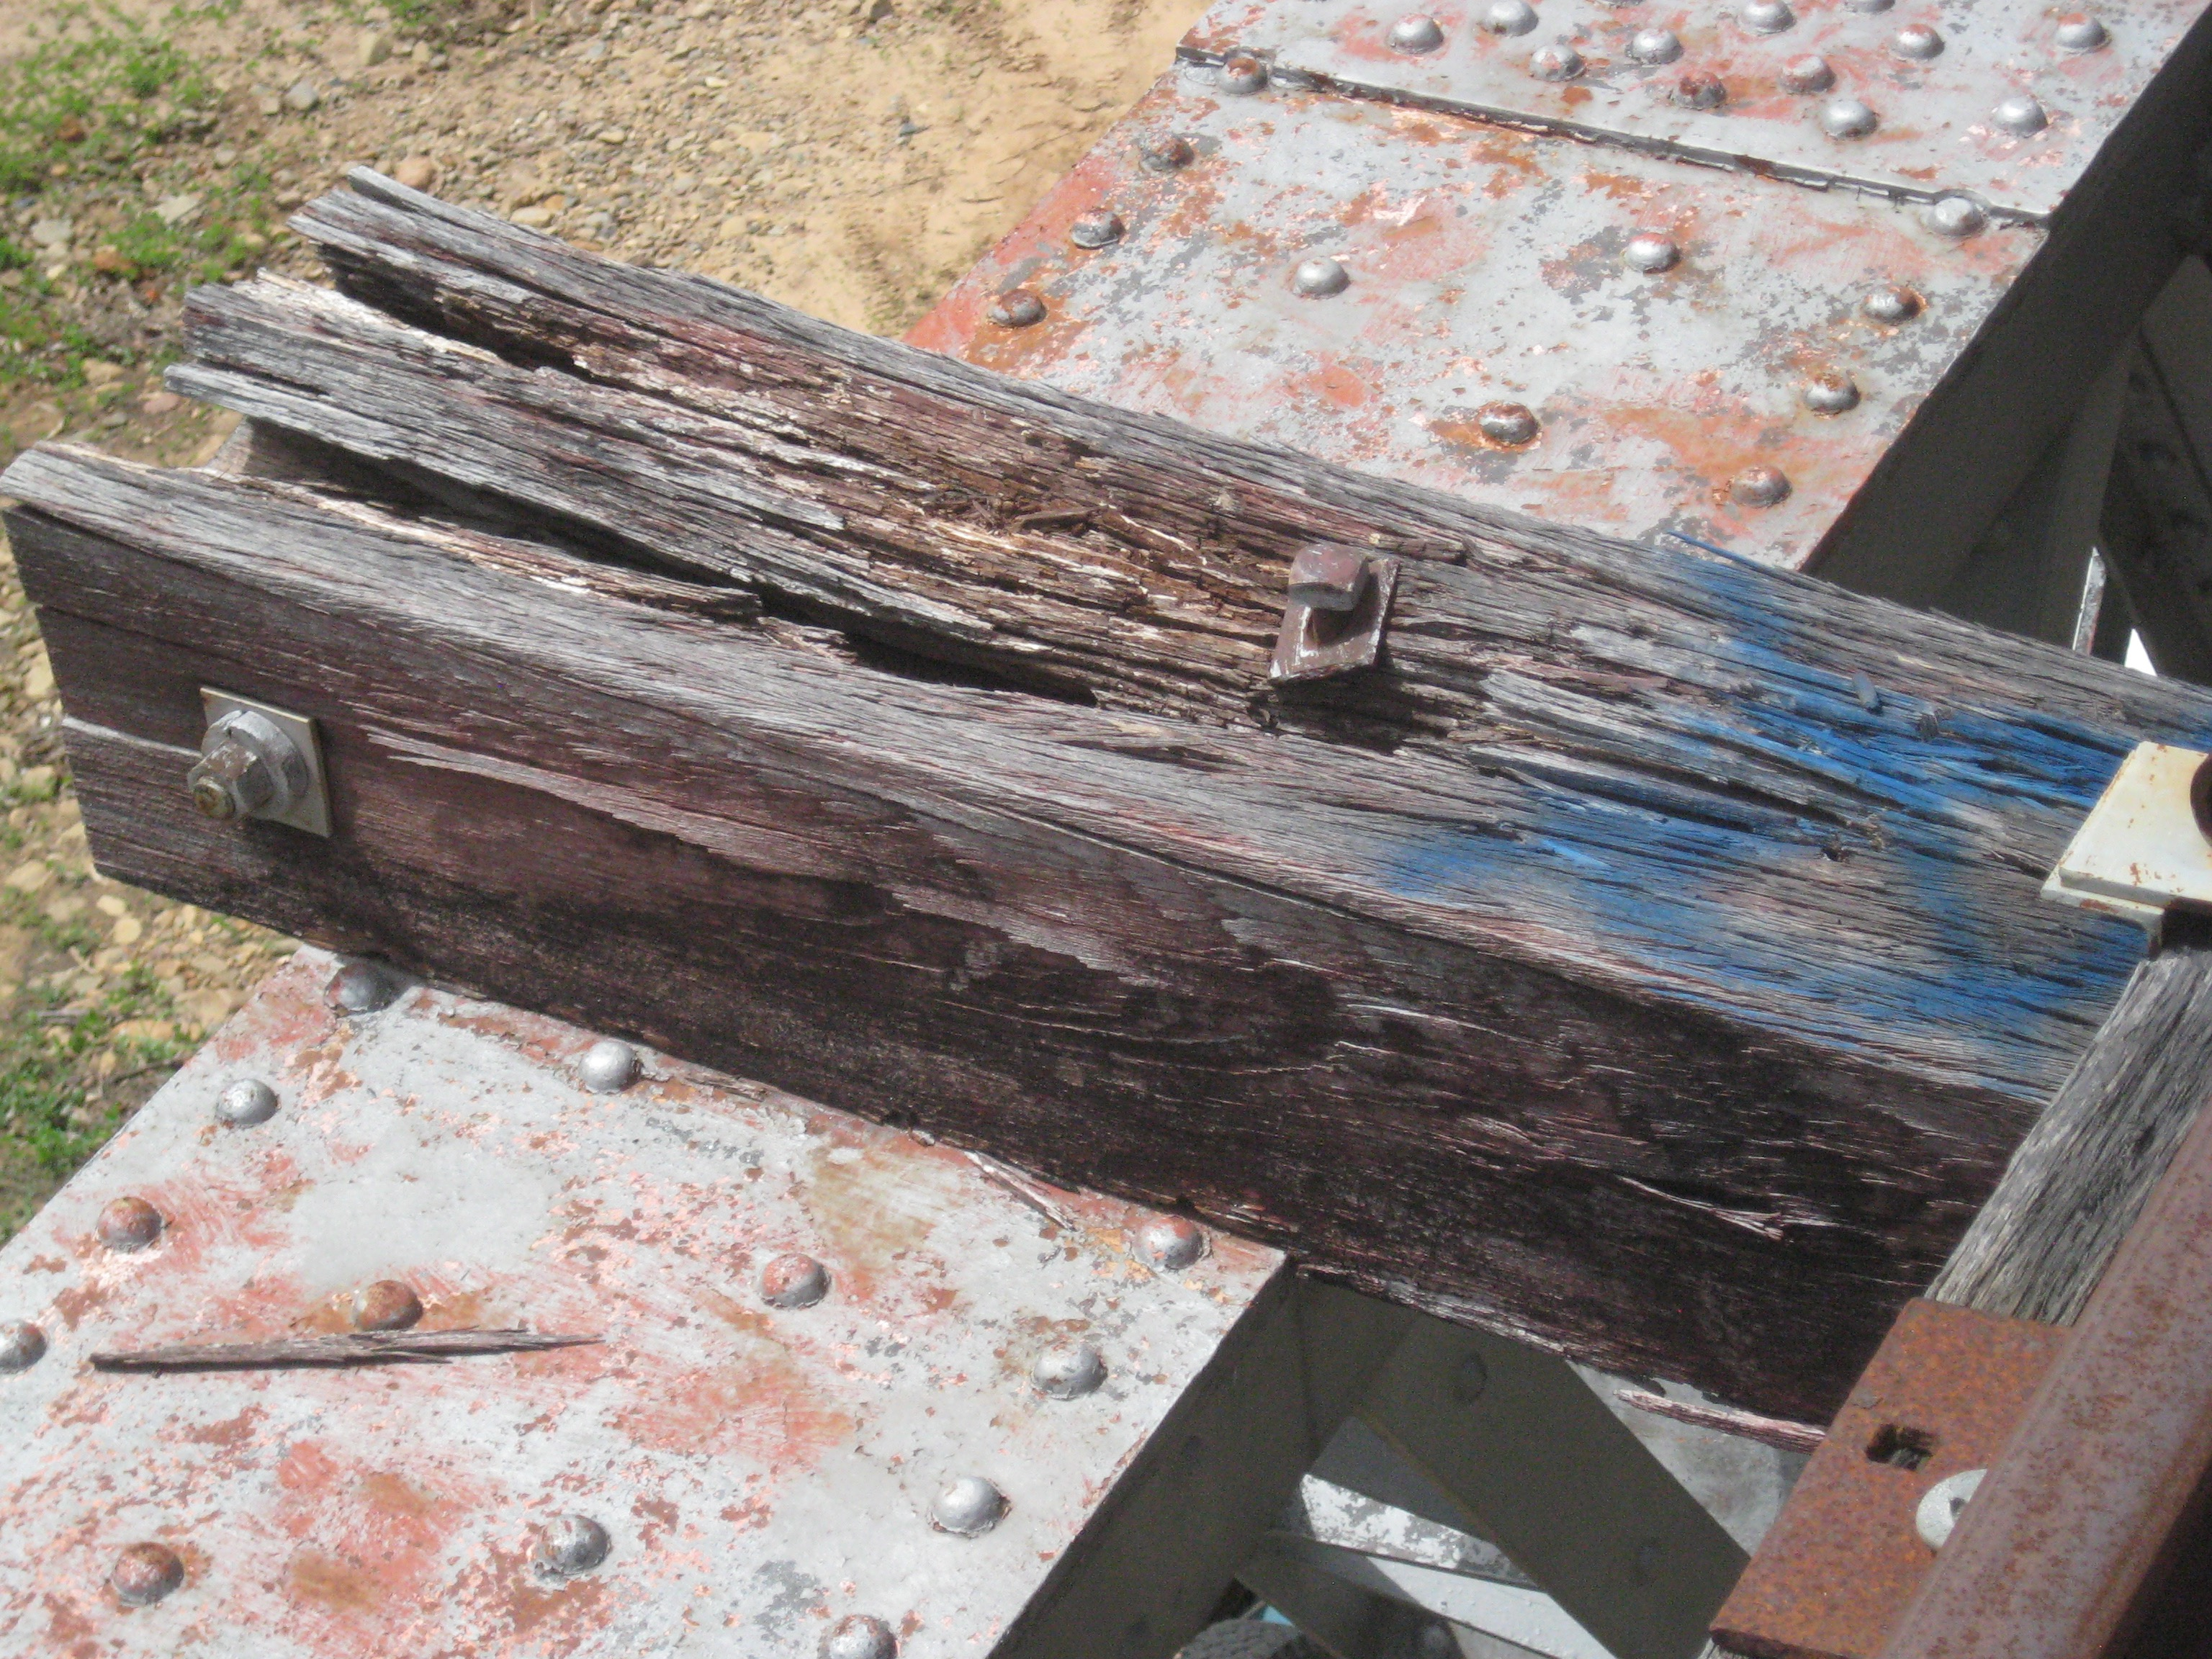
\includegraphics[scale=0.07]{Core_Rotting}
	 		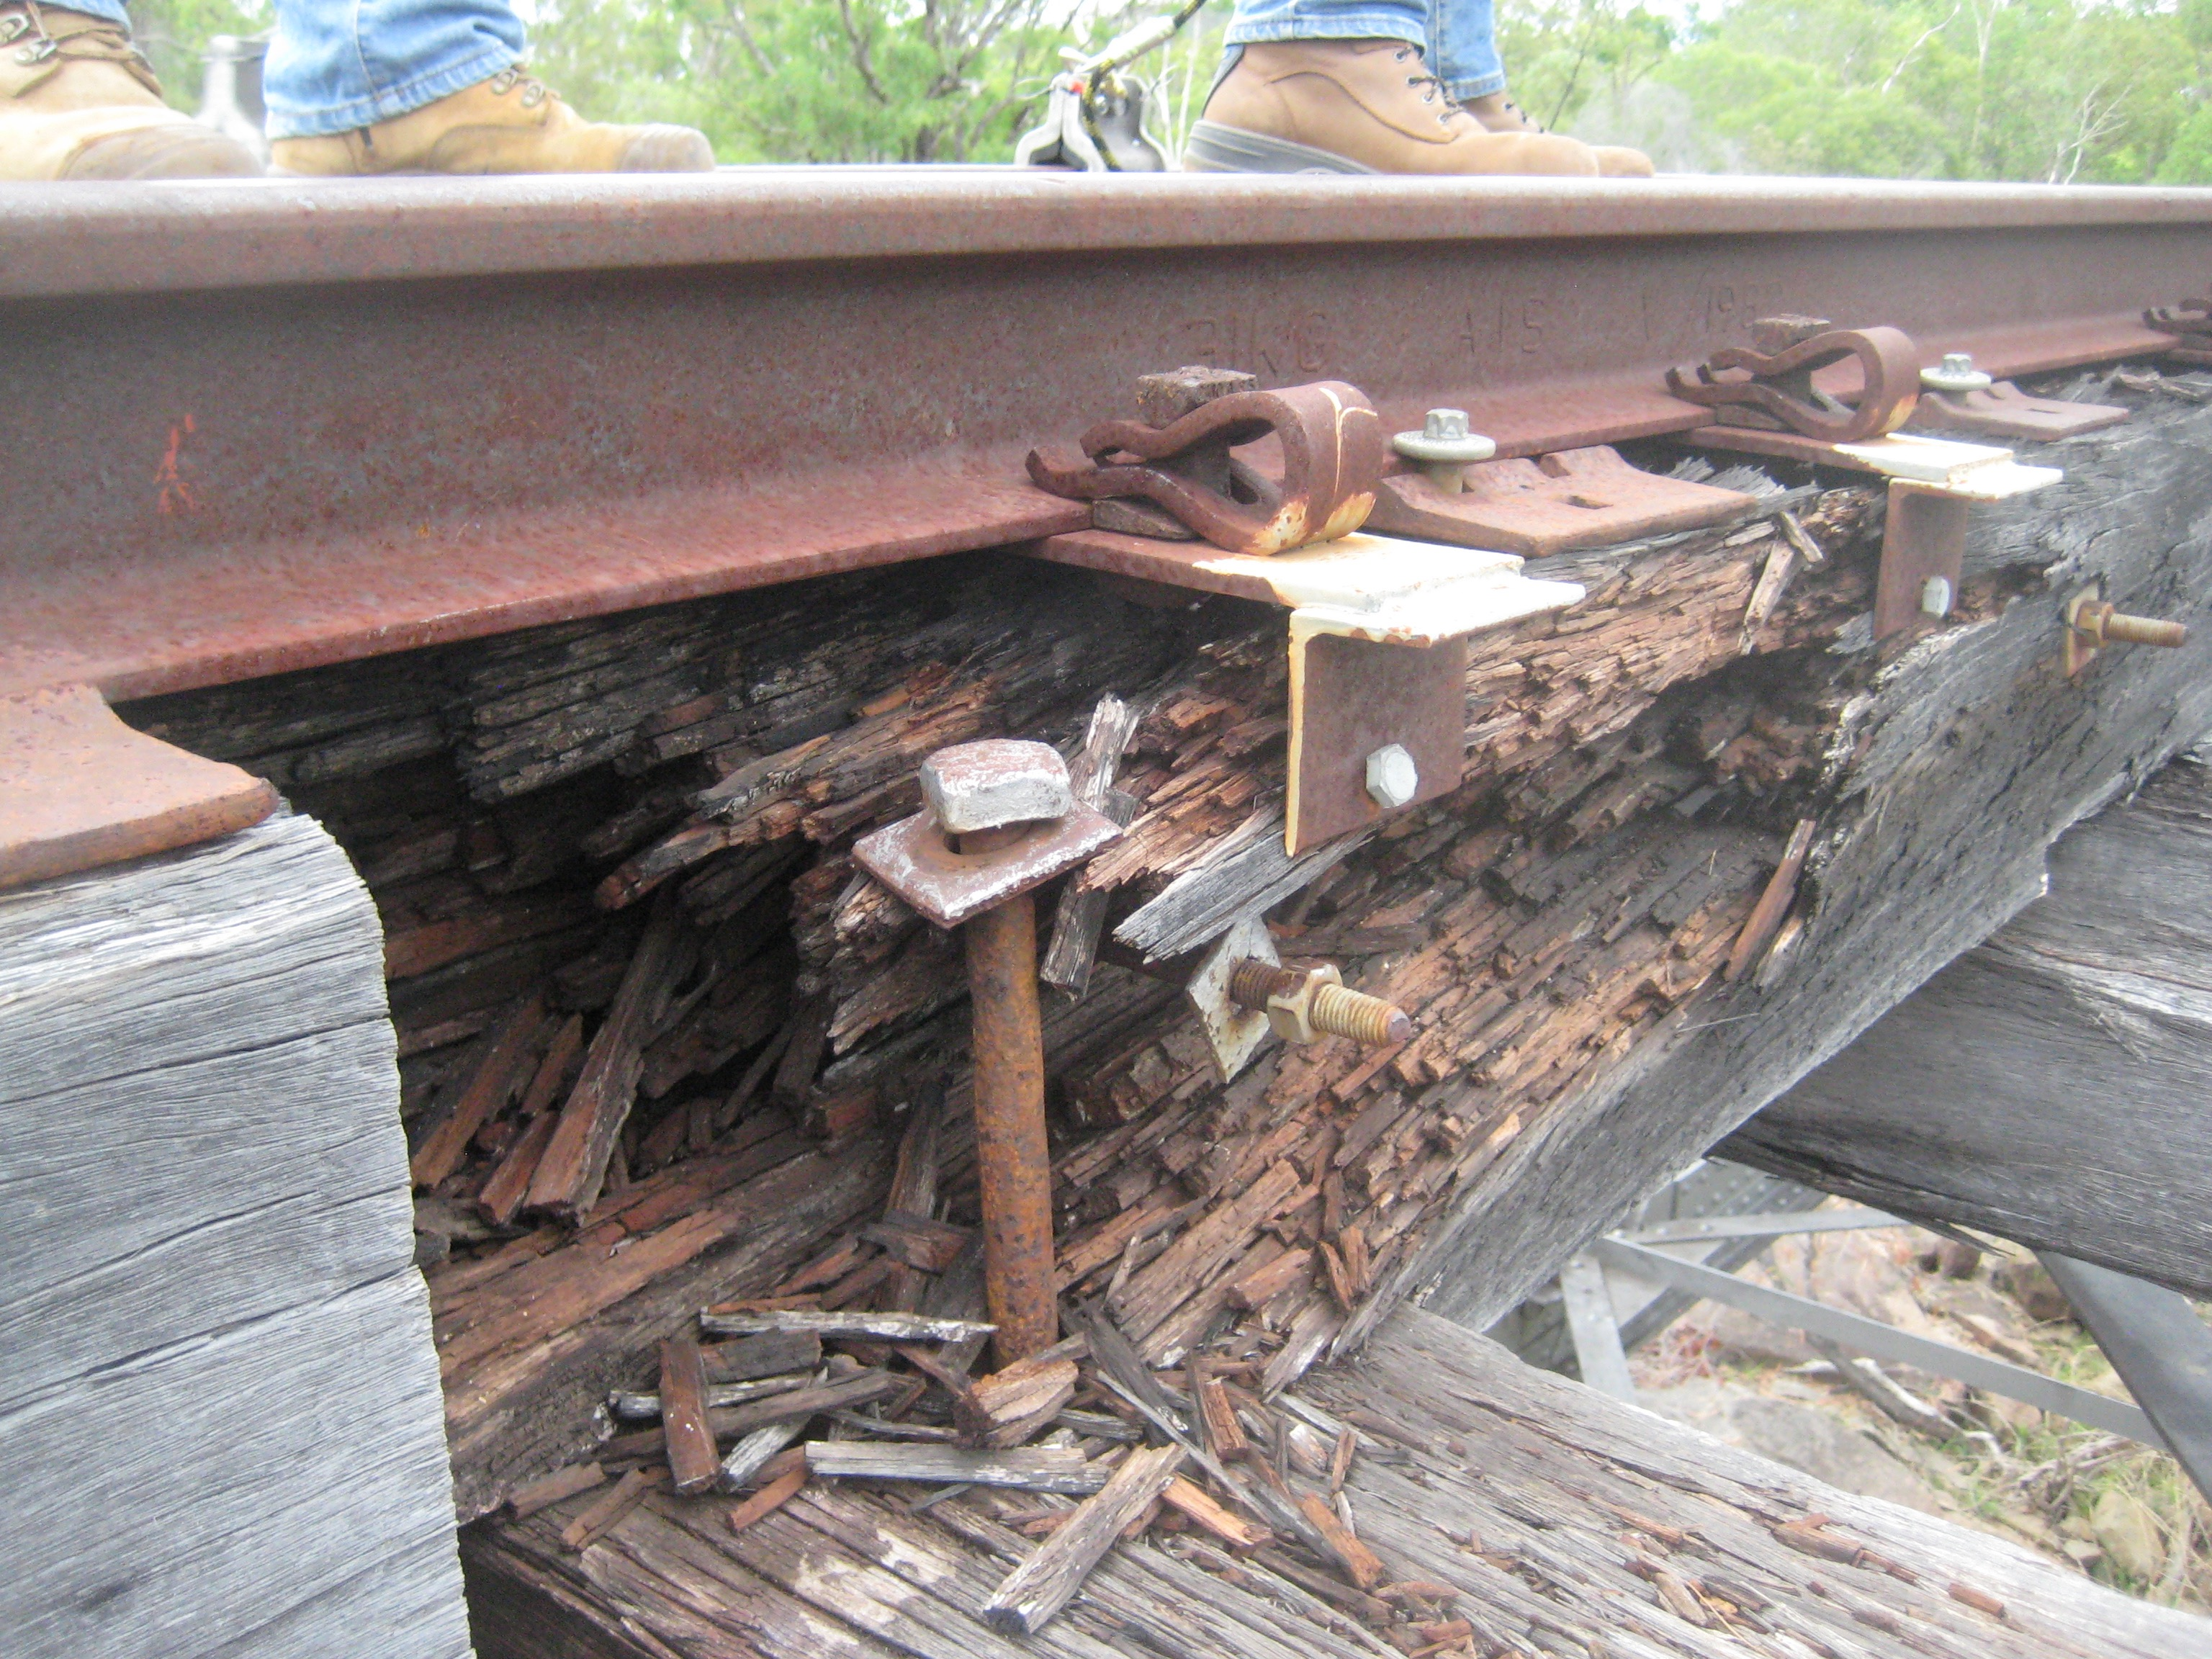
\includegraphics[scale=0.07]{Notch_Rotting}
	 		\caption{Core and Notch Rotting}
	 	    \label{fig:Rot}
	 	\end{figure} 
	
	\noindent
	Rot is decay caused by wood-destroying fungi which requires adequate moisture \cite{heckroodt_guide_2002}, heat and oxygen to prosper. This results in two different types of decay; brown rot and white rot. Brown rot is common in softwood where the fungi attacks only the cellulose creating a brown colour. However, white rot is more common in hardwood and is caused by the fungi attacking both the cellulose and lignin in the wood, creating a white colour. Rotting overall allows the rapid absorption of water and can be identified by a colour change or odor similar to anise or wintergreen\cite{white_bridge_1992}. Both weathering and rotting are effects of long-term exposure to the environment and can lead to a significant reduction in the strength of the member and potentially failure.
	
    \vspace*{\baselineskip}
	    
    \noindent
    \textbf{Insects}\par
    \noindent
    Timber is prone to two main types of insect attack; termite and lyctids. Termites require mois-ture, warm temperatures, access to their nest and usually ground contact to prosper. The most effective way to avoid termite damage is to use a timber species that is resistant to termites. Alternatively, preservative treated timber can be used or a physical or chemical barrier can be created between the timber ends and the nests \cite{_section_2008}.
	
	\vspace*{\baselineskip}
	
	\noindent
	Only the sapwood present in specific hardwoods are vulnerable to lyctids (or powder post beetles), softwoods are resistant to attack from these insects. Thus the use of softwoods or avoidance of the used of certain susceptible hardwoods will reduce the risk on lyctid attack \cite{_section_2008}.
	
	 \vspace*{\baselineskip}
	 
	\noindent
	Both these types of insects cause the same issues in timber; where they tunnel through the wooden members, causing large amounts of intricate bored out networks. This severely reduces the member strength and can eventually cause failure \cite{ryall_bridge_2001}.

	
    \vspace*{\baselineskip}
    
    \noindent
    \textbf{Cracking}
    
    \noindent
    Cracking usually occurs due to applied loads (dead and live) exceeding the strength capacities of the timber member and will eventually lead to failure. This defect can occur in any conditions and is purely dependent on the loads that are applied. However the presence of other capacity reducing defects can significantly increase the chances of cracking. The two types of cracks that occur are flexural and shear cracking \cite{_timber_2005}.
	
    \vspace*{\baselineskip}	
	
	\noindent
	Flexural cracks appear on the areas of a bridge that have high moments due to applied loads. The common location for flexural cracking are at the mid-span of the member, over the support and underneath any other permanent loads (dead loads). These areas are depicted in the Figure \ref{fig:Flex} \cite{_timber_2005}.  

 	\begin{figure}[h]
        \begin{center}
		 	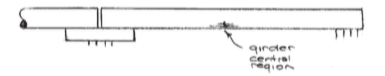
\includegraphics[scale=0.8]{Failure_Location_1}
	 		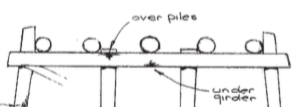
\includegraphics[scale=0.8]{Failure_Location_2}
        \end{center}
	 		\caption{Locations of Flexural Cracking or Crushing \cite{_timber_2005}}
	 		\label{fig:Flex}
	\end{figure}
\pagebreak

    \noindent
	Cracking due to flexure occurs in the tensile region or face of the member and can also result in the occurrence of crushing in the compression region. Hence, flexural cracking can be a combination of tensile and compressive failure \cite{thelandersson_timber_2003}. 

    \vspace*{\baselineskip}	
    
	\noindent
	Shear cracking is caused by the shear capacity of the timber being exceeded by applied loads, resulting in horizontal cracks propagating along the grain, as shown in Figure \ref{fig:Shear}. These cracks occur in high shear stress regions throughout the bridge such as over piles and at the ends of girders \cite{_timber_2005}. 
	
	\begin{figure}[h]
 		\begin{center}
 			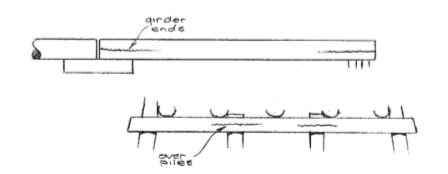
\includegraphics[scale=0.8]{Shear_Failure}
 		\end{center}
 		\caption{Locations of Shear Cracking \cite{_timber_2005}}
 		\label{fig:Shear}
 	\end{figure}
   \noindent 
   Both flexural and shear cracking on bridges is usually a result of bending which can cause forces in tension, compression and shear as well as moments \cite{ritter_timber_1990}. 

\subsection{Timber Properties}
    Timber is a very unique structural material and differs significantly from other man-made materials, such as steel or concrete \cite{plevris_frp-reinforced_1992}. This is due to its fibrous cell structure.
	
	\vspace*{\baselineskip}	
	
	 \noindent
	 The primary forms of failure in timber beams are tensile, shear and compressive failure. For timber, the stress-strain relationship is assumed to be uniaxial \cite{bazan_ultimate_1980,buchanan_combined_1986}, as shown in Figure \ref{fig:Stress-Strain}, where the negative region describes compression and positive region is in tension.
	 
	\begin{figure}[h]
  		\begin{center}
  			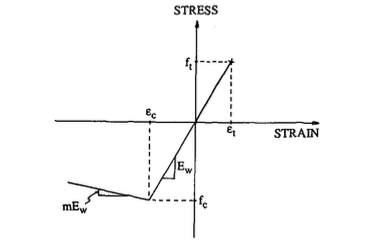
\includegraphics[scale=0.9]{Stress_Strain_Wood}
  		\end{center}
  		\caption{Standard Stress-Strain Diagram of Timber \cite{plevris_frp-reinforced_1992}}
  		\label{fig:Stress-Strain}
  	\end{figure}
	 
	 \noindent
	 The member fails in tension at a stress $f_{t}$, with a relating strain $\varepsilon_{t}$, and in compression fails at a stress $f_{c}$ and strain $\varepsilon_{c}$. The Young's modulus of the wood ($E_{w}$) is the gradient of the stress strain relationship. Beyond the compression-strain at failure ($\varepsilon_{c}$) the gradient and direction of the line changes by a constant ratio m of the Young's modulus \cite{plevris_frp-reinforced_1992,fiorelli_fiberglass-reinforced_2006}.
	 
     \vspace*{\baselineskip}	
	 
	 \noindent
	 Tensile failure is a brittle failure and is usually caused by long-term constant distributed loading. Longer members are more susceptible to tensile failure which occurs at the weakest point on the beam. Compressive failure is also caused by long-term loading and is a ductile failure \cite{thelandersson_timber_2003}. 
	 
     \vspace*{\baselineskip}
	 
   	\noindent
   	Modulus of rupture (MOR) is the maximum allowable stress a species of timber can withstand before its fibres rupture or break; which defines the bending strength \cite{markwardt_strength_1935}. It can be calculated from the maximum load the beam can carry ($F_{R}$) \cite{walker_primary_2013}  and is given by
   	
   	\begin{equation}
   	MOR = \dfrac{M}{Z} 
   	\end{equation}
   	
   	\begin{equation}
   	MOR \approx \dfrac{3 F_{R} l}{2bh^{2}} 
   	\end{equation}
   	
   	\noindent
   	where; \par
   	$ l $ = Span of the beam \par
   	$ b $ = Width of the beam \par
   	$ h $ = Height of the beam. \par
   	$ Z $ = Section modulus \par
   	 
   	\vspace*{\baselineskip}
   	
   	\noindent
   	 The modulus of elasticity (MOE) measures the flexibility or stiffness of timber and is determined through bending and deflection \cite{walker_primary_2013,agriculture_encyclopedia_2007}. The MOE in bending, also commonly denoted as $E_{b}$, can be determined from the load at the proportional limit ($F_{p}$) \cite{agriculture_encyclopedia_2007} and is given by
   	 
   	 \begin{equation}
  E_{b} \approx \dfrac{F_{p} l^{3}}{4 \Delta bh^{3}}
   	 \end{equation}
   		
   	\noindent
   	where; \par
   	$ \Delta $ = Deflection at midspan due to the load $F_{p}$.\par
   	 
   	\vspace*{\baselineskip}
	 
	\noindent 
	 The flexural ability and properties is predominately due to the aspect ratio of the wood. Aspect ratio is the defined as the ratio between the fibre length to the fibre thickness. Longer fibres result in superior mechanical properties compared to shorter fibres, thus a higher aspect ratio renders better flexural properties \cite{klyosov_wood-plastic_2007}.  
	 
	 \vspace*{\baselineskip}
	 
	 \noindent
	 The other form of failure in wood is shear failure, which is again caused by applied shear loads exceeding the shear capacity of the beam. The shear stress distribution of a standard rectangular beam can be seen in Figure \ref{fig:Shear-Stress}, and is of parabolic nature both along and perpendicular to the grain.
	 
	\begin{figure}[h]
		\begin{center}
			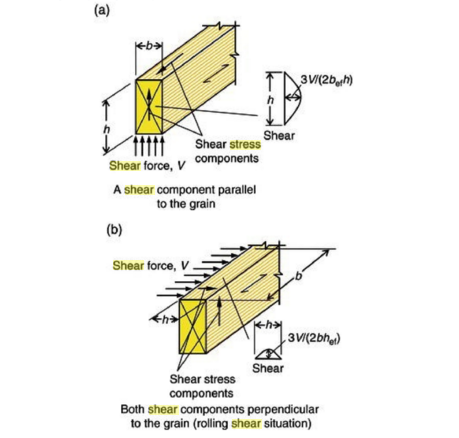
\includegraphics[scale=0.7]{Shear_Stress}
		\end{center}
		\caption{Shear Stress Distribution \cite{porteous_structural_2013}}
		\label{fig:Shear-Stress}
	\end{figure} 
	
	\pagebreak
	 
	 \noindent
	 The shear capacity of a timber species is a measure of the timber fibre's ability to withstand slippage. Shear capacity in timber is much greater across the grain than along the grain, where the fibres have to be broken, than along the grain where the fibres only need to be separated from each other \cite{walker_primary_2013}.
	
	
	\subsection{Australian Member Design}
	There are three common cross-sectional shapes of members in bridge construction; rectangular, circular and octagonal. The most commonly used is the rectangular section member, mainly for smaller scale constructions (e.g. frames, foot-bridges, etc.). However, for bridges requiring a large strength capacity, such as a rail bridge, the log can not be substantially reduced in size, as done to achieve rectangular cross-sections, thus the round and octagonal members are required. 
	
	
	\subsubsection{Rectangular Section}
	There are three standard Australian design codes that discuss design processes and equation for rectangular timber members; AS1720.1, AS4676 and AS4063. 

	 \vspace*{\baselineskip}
	 
	\noindent
	\textbf{Bending}\par
	% Discuss design aspects of a rectangular section member
	% Show equations and explain design process and necessary factors
	% Include all necessary tables and graphs
	
	\noindent
	The bending capacity ($M_{d}$) for an un-notched beam, with a rectangular section, is given in AS1720.1 as
	\begin{equation}
	\phi M_{d} = \phi k_{1} k_{4} k_{6} k_{9} k_{12} f'_{b} Z
	\end{equation}
	
	 where 
	 
	 $ \phi $ = Capacity Factor\par
	 
	 $ k_{1} $ = Duration of Load Factor\par
	 
	 $ k_{4} $ = Moisture Condition Factor\par
	 
	 $ k_{6} $ = Temperature Factor\par
	 
	 $ k_{9} $ = Strength Sharing Factor\par
	 
	 $ k_{12} $ = Slenderness Factor\par
	 
	 $ f'_{b} $ = Characteristic value for bending for section size
	 
	 $ Z $  = Section modulus of beam about bending axis.
	
	\vspace*{\baselineskip}
	
	\noindent
	All factors and the strength characteristic for bending can be determined from AS1720.1.
	
	\vspace*{\baselineskip}
	
	\noindent
	\textbf{Shear}\par
	
	\noindent
	The design capacity in shear of un-notched beams is described by AS1720.1 as
	\begin{equation}
	V_{d} = \phi k_{1} k_{4} k_{6} f'_{s} A_{s}
	\end{equation}
	
	\noindent
	where $\phi$, $k_{1}$, $k_{4}$, and $k_{6}$ are as determined for bending capacity design, \par
	
	$ f'_{s} $ = Characteristic value in shear\par
	
	$ A_{s} $ = Shear plane area.\par
	
	\vspace*{\baselineskip}
	
	\noindent
	and the characteristic value in shear can be found in AS1720.1. \par
	
	\vspace*{\baselineskip}
	
	\noindent
	Also when the beam is loaded about its major axis in bending, the shear plane area can be found from the breadth (b) and depth (d) using
	\begin{equation}
	A_{s} = \dfrac{2bd}{3}
	\end{equation}
	
	\subsubsection{Circular Section}
	The amount of information and research surrounding circular section members are minimal, and there are few design equations determined specifically for these members. 
	
	\vspace*{\baselineskip}
	
	\noindent
	\textbf{Bending}\par
	% Discuss design aspects of a circular section member
	% Show equations and explain design process and necessary factors
	% Include all necessary tables and graphs
	\noindent
    AS1720.1 uses the rectangular formula with additional factors to account for the change in section shape. This formula and additional factors are
	\begin{equation}
	\phi M = \phi k_{1} k_{4} k_{6} k_{9} k_{12} k_{20} k_{21} k_{22} f'_{b} Z
	\end{equation}

    \noindent
    where $\phi$, $k_{1}$, $k_{4}$, $k_{6}$, $k_{12}$ are as for working rectangular design and \par
    
    $ k_{20} $ = Immaturity Factor\par
    
    $ k_{21} $ = Shaving Factor\par
    
    $ k_{22} $ = Processing Factor.\par
	
	\vspace*{\baselineskip}
		
	\noindent
	\textbf{Shear}\par
	\noindent
	The design shear capacity given by AS1720.1 is again a modification of the rectangular design approach and is given by 
	
	\begin{equation}
	V_{d} = \phi k_{1} k_{4} k_{6} k_{20} f'_{s} A_{s}
	\end{equation}
	
	\noindent
	where the factors, $f'_{s}$ and $A_{s}$ are as specified in rectangular design, and $k_{20}$ takes into account the maturity of the material. The shear plane area for a round member is\par
	
	\begin{equation}
	A_{s} = \dfrac{3\pi d^{2}}{16}
	\end{equation}
	
	
	\noindent
	
	\subsubsection{Octagonal Section}
    Queensland Department of Transport and Main Roads (TMR) suggests that the design of such members for bending, is the same as for rectangular sections \cite{_timber_2005}. However there is very little information surrounding octagonal member design and no design methods determined specifically for this cross-section.


	\subsection{Notching}
	Notching or sniping is when the lower corner of a member is cut to make insertion easier, and to increase the stability of the member when sitting on a pier/abutment. One of the major issues faced with notches are they significantly reduce the load-carrying and shear capacities of timber beams. For these reasons, it is suggested that the use of notches be avoided in practice, however in some situations they cannot be \cite{jockwer_state---art_2013,jockwer_structural_2014}.
	
	\vspace*{\baselineskip}
	
	\noindent
    The reduction in the shear capacity of the beam causes a brittle failure and cracking to initiate from the corner of the notch, and propagate along the direction of the grain \cite{jockwer_state---art_2013,_timber_2005}. Figure \ref{fig:Notch_Crack} indicates the common behaviour of notch cracking.
    
       	\begin{figure}[h]
       		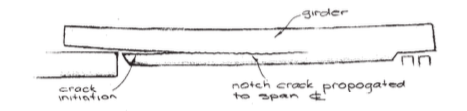
\includegraphics[scale=0.9]{Shear_Failure_Notching}
       		\caption{Notch Cracking \cite{_timber_2005}}
       		\label{fig:Notch_Crack}
       	\end{figure}
       
	\noindent
	To reduce the effects of capacity loss, TMR limit the section area loss from notching to be a maximum of 10\%. In cases where the notch is strengthened, a maximum allowable section loss can be up to 25\% \cite{_timber_2005}. As shown in Figure \ref{fig:Bending}, TMR also specifies that if there is less than 75\% of the original depth over the support, there is a high chance of failure to occur in bending. 
	
	       	\begin{figure}[h]
	       		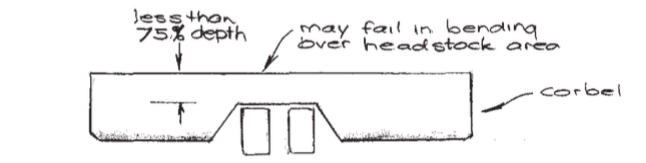
\includegraphics[scale=0.7]{Bending_Fail}
	       		\caption{Member failure in bending over support \cite{_timber_2005}}
	       		\label{fig:Bending}
	       	\end{figure}
	
	\pagebreak
	
	\noindent
	There are three different types of fracture modes of a notch in a timber member which are dictated by the forces/stresses present at the notch corner. Figure \ref{fig:Frac_Mode} depicts these modes.

	       	\begin{figure}[h]
	       		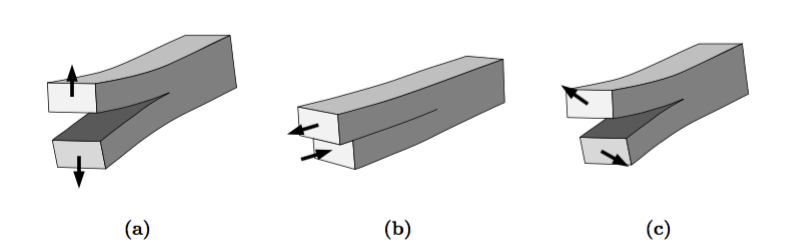
\includegraphics[scale=0.53]{Fracture_Modes}
	       		\caption{Fracture Modes (a) mode 1  (b) mode 2  (c) mode 3 \cite{jockwer_structural_2014}}
	       		\label{fig:Frac_Mode}
	       	\end{figure}
	
	\noindent
	Fracture mode 1 is when the crack propagating from the notch opens and is caused by tensile forces at the notch corner. Mode 2 is horizontal cracking/shearing, cause by shear forces acting along the grain at the notch corner. Lastly, mode 3 is a mixed mode fracture and is caused by a combination of both tension and shear forces \cite{jockwer_structural_2014}. 
	
	\subsubsection{Notch Types}
	There are four main types of notching, rectangular end notch, tapered end notch, rounded end notch and notch in span. The figure below shows the geometry of each type of notch.
	
	\begin{center}
		\begin{figure}[h]
			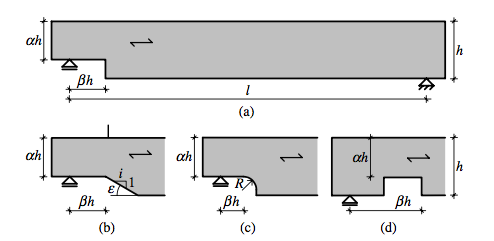
\includegraphics[scale=0.9]{Notch_Types}
			\caption{Notching Types; (a) rectangular end notch; (b) tapered end notch; (c) rounded end notch; (d) notch in span \cite{jockwer_state---art_2013}}
		\end{figure}
	\end{center}
	

	\noindent
	There is little information surrounding the exact effects of each type of notch on members. However, it is recommended by Australian Standard AS1720.1 that a tapered notch with a 1:4 gradient chamfer from the notch corner be used if notching is required. In theory, this particular tapered notch will increase the member's shear capacity by three times in comparison to a rectangular end notch\cite{_timber_2005}. 
	
	
	\subsubsection{Notch Design}	
	There are many different methods for designing notched members, based on significantly different concepts and, in most cases, obtaining varied results \cite{jockwer_structural_2014}. There are few methods in designing round end notches and notches within member spans, and most standards only design for a rectangular or tapered notch. However, the greatest limitation in notch design is all methods are based on rectangular section beams and do not account for circular or octagonal sections \cite{_timber_2005}. This is a major issue, as round and octagonal sections are preferred in timber bridges, due to their larger sections. 
	
	\vspace*{\baselineskip}
	
	\noindent
	\textbf{Australian Standards}\par
	\noindent
	The notched member design method used in AS1720.1 focuses on stress intensities and accounts for the effects of the maximum bending moment ($M^{*}$) and maximum shear force ($V^{*}$) occurring at the corner of the notch; where any negative values for bending moment or shear are neglected  \cite{jockwer_structural_2014}. AS1720.1 notch design equation is
	
	\begin{equation}
    \dfrac{6M^*}{bd_n^2} + \dfrac{6V^*}{bd_n} \leq \phi g_{40} k_1 k_4 k_6 k_{12} f'_{sj}
    \label{eq:Aus}
	\end{equation}
	
	\noindent
	where \par
	$ f'_{sj} $ = Shear strength\par
	$ g_{40} $ = Notch coefficient.\par
	
	\vspace*{\baselineskip}
	
	\noindent
	The k-factors and $\phi$ are purely dependent on location, use and specific timber characteristics, and are found as per usual design methods in AS1720.1. The other variables used in equation \ref{eq:Aus} are depicted in Figure \ref{fig:figure2}.
	
	\begin{center}
		\begin{figure}[h]
			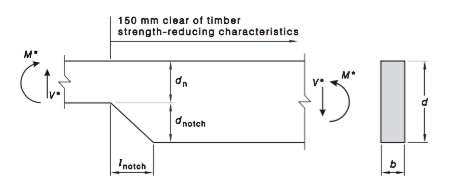
\includegraphics[scale=0.9]{Notching.png}
			\caption{Notation for Notch}
			\label{fig:figure2}
		\end{figure}
	\end{center}
	
	\pagebreak
	
	\noindent
	The notch coefficient g40 depends on the taper and height of the notch and can be found according to Table \ref{tab:g40}.
	
	\begin{center}
		\captionof{table}{Notch Coefficient}
		\label{tab:g40}
		\begin{tabularx}{\textwidth}{>{\centering}X|>{\centering}X|>{\centering}X} 
			\hline \hline
			\multirow{2}{*}{\textbf{Notch Angle Slope}} & \multicolumn{2}{c}{$g_{40}$} \\
			\cline{2-3}
			
			&$d_{notch} \geq 0.1d$ & $d_{notch} < 0.1d$ \tabularnewline [0.5ex] 
			\hline
			$l_{notch}/d_{notch}=0$ & $9.0/d^{0.45}$ & $3.2/d^{0.45}_{notch}$ \tabularnewline [0.5ex]
			\hline
			$l_{notch}/d_{notch}=2$ & $9.0/d^{0.33}$ & $4.2/d^{0.33}_{notch}$ \tabularnewline [0.5ex]
			\hline
			$l_{notch}/d_{notch}=4$ & $9.0/d^{0.24}$ & $5.2/d^{0.24}_{notch}$ \tabularnewline [0.5ex]
			\hline \hline
		\end{tabularx}
	\end{center}
	
	\vspace*{\baselineskip}
	
    \noindent
	AS1720.1 specifies that for this design method, no strength-reducing characteristics, such as knots, are allowed within 150mm from the notch corner.
	\vspace*{\baselineskip}
		
	\noindent
	Australian design method is based on LEFM, which is basic fracture mechanic concepts under the assumptions that the material is linearly elastic. However this assumption is not ideal for timber, as it's elastic properties are considered orthotropic. 
	
	\vspace*{\baselineskip}
	
	\noindent 	
	\textbf{Fracture Mechanics}\par 	 	
	\noindent 	
	The AS1720.1 notched member design method considers only the effect of stress intensities and does not take into account fracture mechanics. In 1988, Gustafsson proposed an equation to design for strength of the notch, based on fracture energy \cite{jockwer_state---art_2013,gustafsson_study_1988}.  	 \begin{equation} 
	\dfrac{V_{f}}{b\alpha d} = \dfrac{\sqrt{\frac{G_{c}}{d}}}{\sqrt{0.6\frac{(\alpha-\alpha^{2})}{G_{xy}}}+\beta\sqrt{6\frac{(1/\alpha-\alpha^2)}{E_{x}}}} \end{equation} 		 		 		
	\noindent 		
	Where; \par 	
	$ V_{f} $ - Shear force at fracture of notch\par 	
	$G_{xy}$ - Shear modulus\par  	
	$ E_{x} $ - Modulus of elasticity in beam direction, parallel to the grain\par 	
	$ d $ - depth of the member\par  	
	$ G_{c} $ - Fracture energy\par  	
	$ \beta $, 
	$ \alpha $ and h are depicted in the figure below. \par 		 	
	\vspace*{\baselineskip} 	 	
	\noindent 	This equation was established for a beam notched at both ends, and in accordance with the characteristics shown in the figure \ref{fig:Gust}. The actions due to the moment and shear, along with the effect from elastic clamping, results in a deflection, which is the basis of this fracture energy approach. Gustafsson derived this deflection, also considering lower bending stiffness of the cross-section at the junction of the notched part of the beam, and assumed its proportionality to the moment acting at the notch corner \cite{jockwer_state---art_2013}. Clamping was also incorporated with a factor, which was conservatively chosen as $1/\alpha^{3}$ \cite{gustafsson_study_1988}.   
		 	 		
		\begin{figure}[h] 			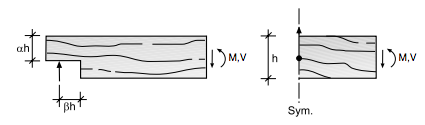
\includegraphics[scale=0.9]{Geom_notched_beam_dowl} 			\caption{Geometry of notched beam and dowel joint \cite{serrano_fracture_2007}} 	
		\label{fig:Gust}	
		\end{figure} 	
	 		 	
	\noindent 	
	The fracture energy for a notched member can be found using the following equation \cite{serrano_fracture_2007}.  	 	
	\begin{equation} 		
	G_{c} = \dfrac{1}{2}(P_{f}^{2}/B) \dfrac{dC(a)}{da}  	\end{equation} 	 	
	Where;\par 	
	C - denotes the compliance of the structure\par 	
	da - extension of the length of the crack\par 	
	$P_{f}$ - magnitude of load that start propagation of the crack\par 	
	B - width of the fracture area (i.e. $B = dA/da$) 
	   
	 \vspace*{\baselineskip} 	 	
	 
	 \noindent 
	 Similar notch strength equations have been derived (Smith et al. 1996), with a defining difference of the clamping effect. Smith et al proposed a notch strength relationship from the same fracture mechanic concepts, but taking a clamping factor of $1/\alpha^{2}$. It has been found through comparison, that the prediction of the notch strength proposed by Gustafsson was more conservative and accurate than Smith et al. which has given results exceeding the notches capacity \cite{jockwer_state---art_2013}.   	
	 
	 \vspace*{\baselineskip} 	 	
	 
	 \noindent 	This approach is used as a verification of the shear stress in the notch cross-section and has become a basis for design methods in European and Canadian design codes.
	
	\vspace*{\baselineskip}
	
	\noindent
	\textbf{Eurocode 5 Approach}\par
	
	\noindent
	The European timber structure design code (Eurocode 5) is based on studies of notch fracture mechanics and specifies the following equation for notch design as
	 
	\begin{equation}
	\tau_{d} = 1.5\dfrac{V}{b h_{ef}} \leq k_{v} f_{v,d} 
	\end{equation}
     
     where\par
     $ \tau_{d} $ = Shear stress \par
     $ V $ = Shear force \par
     $ h_{ef} $ = Depth above notch \par    
     
     \vspace*{\baselineskip} 
     
     \noindent
     The shear strength, $ f_{v,d} $, can be found using
     
   	\begin{equation}
   	f_{v,d} = \dfrac{k_{mod} f_{v,k}}{\gamma M} 
   	\end{equation} 
     
     \noindent
     where $f_{v,k}$ is the characteristic shear strength, $k_{mod}$ is a strength modification factor and $\gamma M$ is a material modification factor, all of which can be found in Eurocode 5 \cite{_eurocode_1995}.
     
     \vspace*{\baselineskip} 
     
     \noindent
     The notch factor $k_{v}$ is derived from Gustafsson's 1988 equation \cite{gustafsson_study_1988}, as well as modifications to account for the taper of the notch ($i$) established by Riberholt \cite{riberholt_timber_1991} and is given by
     
     \begin{equation}
     k_{v} = min
     \begin{cases}
	 1  \\ 
	 \frac{k_{n}(1+\frac{1.1i^{1.5}}{\sqrt{h}})}{\sqrt{h}(\sqrt{\alpha(1-\alpha)} + 0.8\frac{x}{h} (\sqrt{\frac{1}{\alpha}-\alpha^{2}})}
    \end{cases}
    \end{equation}
	
	\vspace*{\baselineskip}
	
	\noindent
	Overall, the notch factor considers the notch taper $i$, material constant $k_{n}$, ratio of depth above notch to total depth $\alpha$, the distance to the support $x$, and the total depth of the beam h \cite{_timber_2005,jockwer_structural_2014}.
	
	\vspace*{\baselineskip} 
	
	\noindent
	\textbf{CSA O.86 Approach}\par
	
	\noindent
     The Canadian design code (CSA 0.86:2014) is also based on fracture mechanics and thus has a similar design concept to Eurocode 5 \cite{jockwer_structural_2014}. However, the design is based around the verification of the resistance of the notch ($F_{r}$) instead of the stresses, which is calculated by
     
	\begin{equation}
	F_{r} = \Phi F_{f} A K_{N} 
	\end{equation}     
     
     where\par
     $ \Phi $ = Resistance factor (given as 0.9) \par
     $ A $ = Cross-sectional area
     
     \vspace*{\baselineskip}
     
     \noindent
     $F_{f}$ can be calculated from $f_{f}$ and Equation \ref{eq:Ff} \cite{_csa_2014,_errata:_2013}.
     
   	\begin{equation}
   	F_{f} = f_{f} K_{D} K_{H} K_{Stp} K_{T}
   	\label{eq:Ff} 
   	\end{equation}  
     
     \noindent
     Where $f_{f}$ is given as 0.5MPa for sawn lumber and the condition ($K$) values can be found in CSA O.86.
 
     \vspace*{\baselineskip}
    
     \noindent    
     $K_{N}$ is the notch factor and can be found using Equation \ref{eq:kn} \cite{jockwer_structural_2014,_csa_2014}. The notch factor is based on studies by Smith and Springer, and takes into account the depth of the beam ($d$), notch ratio $\alpha$ and notch length ratio $\eta$ \cite{smith_consideration_1993}.
     
	\begin{equation}
	K_{N} = \bigg\{0.006d \bigg[1.6 \bigg(\dfrac{1}{\alpha}-1 \bigg)+\eta^{2} \bigg(\dfrac{1}{\alpha^{3}}-1\bigg) \bigg] \bigg\}^{-1/2} 
	\label{eq:kn}
	\end{equation} 
    
    where\par
    $ d $ = Total depth of member \par
    $ d_{n} $ = Depth of notch \par
    $ e $ = Length to notch from centre of support \par
    $\alpha = 1 - d_{n}/d$ \par
    $\eta = e/d$ \par
 
    \vspace*{\baselineskip}

    \noindent
    To satisfy CSA O.86 design requirements, the design shear load ($Q_{f}$) must be less than the notch resistance load ($F_{r}$) \cite{_csa_2014,_errata:_2013}. This method only considers the effects of a rectangular end notch (slope 1:0), and does not account for different notch angles.  

\subsection{Timber Strengthening}
There are many methods used to strengthen timber structures \cite{plevris_frp-reinforced_1992}. These techniques are based around combining various different forms of reinforcement to the members. Basic forms of reinforcement have been utilised such as steel bars, steel and aluminium plates and externally bonded plywood. There have also been some slightly more complex strengthening efforts. In 1965, Peterson \cite{leicester_size_1969} attempted to prestress glulam timber beams using stressed steel plates. This was achieved by fixing the steel plates to the tension side of the glulam beam using epoxy. Others include pre-stressing glulam using cable and strengthening using steel tension bearing embedded wire. 

\vspace*{\baselineskip}

\noindent
A popular form of reinforcement of timber beams is the use of fibre reinforced polymers (FRP) composites. This form of reinforcement is unique because of its ability to improve structural strength, stiffness and ductility characteristics, maintaining a very light weight \cite{plevris_frp-reinforced_1992}. Although many methods of timber strengthening has been tested, there are few recorded efforts in testing strengthened notched timber members. 


\subsubsection{Strengthening of Notched Beams}
Due to the abrupt change in the section area from a notch, high stresses are concentrated at the corner of the notch and can develop cracks. Extensions of these cracks can lead to failure and thus reinforcing notches is required to reduce the risk of cracking \cite{jockwer_structural_2014}. Notches can be reinforced either internally (Figure \ref{fig:Internal}) or externally (Figure \ref{fig:External}). Internal reinforcements are usually screwed/glued in rods and fully threaded screws. It should be noted that the screws and rods must be tight fitting to reduce the impact of shrinkage and water penetrating the hole\cite{jockwer_structural_2014,fawwaz_structural_2012}. 

	\begin{center}
		\begin{figure}[h]
			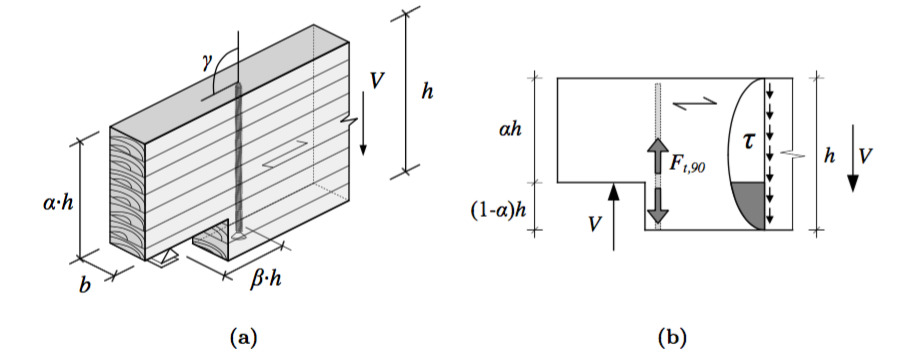
\includegraphics[scale=0.5]{Notch_Screw}
			\caption{(a) Parameters of internal reinforcement  (b) The theoretical portion of the shear stress taken by the reinforcement  \cite{jockwer_structural_2014}}
			\label{fig:Internal}
		\end{figure}
	\end{center}
	
\vspace*{\baselineskip}
	
\noindent
Bolts have been used as a standard notch strengthening method by TMR and are commonly M24 galvanised bolts, inserted perpendicular to the grain and extending through the full depth of the member. A 3mm thick plate is used at either end of the bolt to reduce cracking and pull out effects. The bolts are threaded at both ends and held on by nuts as shown in Figure \ref{fig:Internal2} \cite{_timber_2005}

	\begin{center}
		\begin{figure}[h]
			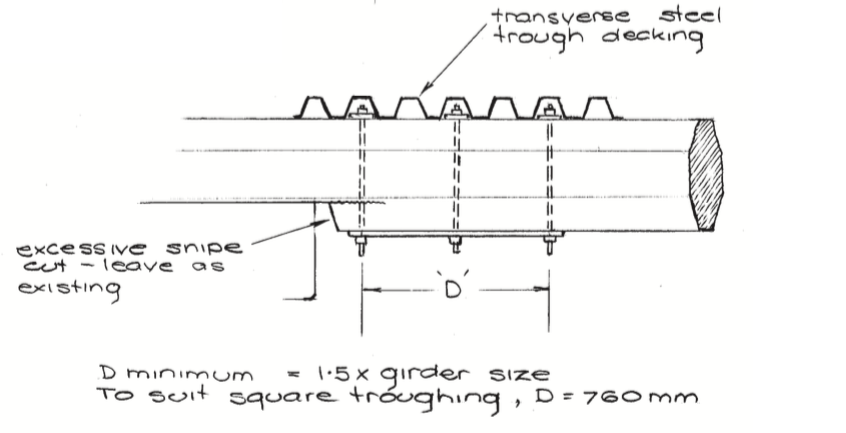
\includegraphics[scale=0.5]{Bolt_Layout}
			\caption{TMR Standard Bolt Layout \cite{_timber_2005}}
			\label{fig:Internal2}
		\end{figure}
	\end{center}
	

\noindent
External notch reinforcement methods are commonly adhered plywood, LVL or lamellas of solid timber and metal plate fasteners \cite{jockwer_structural_2014,fawwaz_structural_2012}. These are used to increase the strength capacities of the notch corner and reduce the risk of cracking. 

\vspace*{\baselineskip}

\noindent
Steel straps have also been used by TMR to reduce notching effects on piles, as seen in Figure \ref{fig:External}. However this method has not been used to reinforce girders. Essentially, a strap works similarly to a plate or wrap, where is compacts the notch corner and reduces the effects from notch cracking. 

	\begin{figure}[h]
		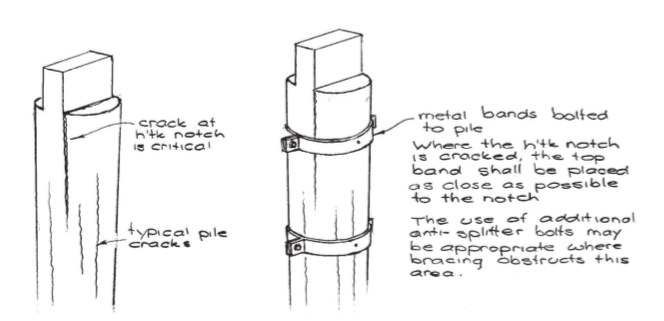
\includegraphics[scale=0.6]{Piles}
		\caption{Straps on Piles \cite{_timber_2005}}
		\label{fig:External}
	\end{figure} 
	\pagebreak

\noindent
In both external and internal reinforcement methods, studies have been undertaken where the material has been replaced with fibre reinforcement polymers (FRP) \cite{jockwer_structural_2014}. However these studies were carried out on rectangular sectioned beams and there is no recorded studies on the effects of notch reinforcement on circular members. 

\subsection{Analysis and Modelling}
For analysis and modelling purposes, timber can be assumed to have orthotropic properties in the longitudinal, tangential and radial directions \cite{kim_modeling_2010}. These directions are shown in Figure \ref{fig:Axes} with relation to the cross-sectional grain direction, where $L$ refers to longitudinal, $R$ to radial and $T$ tangential. This will assist in developing accurate models using finite element analysis (FEA) of a three-dimensional member. 

\begin{figure}[h]
	\begin{center}
		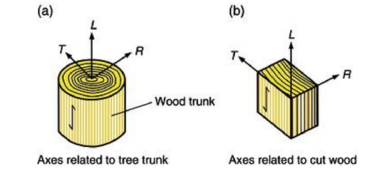
\includegraphics[scale=0.9]{Wood_Axes}
	\end{center}
 	\caption{Wood Axes \cite{porteous_structural_2013}}
 	\label{fig:Axes}
\end{figure}

\vspace*{\baselineskip}
\pagebreak

\section{Materials and Methodology}
Notches are widely used throughout timber bridge construction as a method of seating over other members or piers. Due to the section loss caused by notching, horizontal splitting commonly occurs along the grain, which may result in failure. This is caused by high stresses occurring in the notch corners, particularly in shear, combined with a loss of member capacity due to the reduced area. Although there are design methods for notching, they differ between codes and are based on rectangular sections. This is a major issue as members commonly used in timber bridges are of circular section. To achieve a better understanding of notch behaviour and current design methods, the following experiments and numerical testing were undertaken. 

	\begin{enumerate}
		\item Small scale tests on rectangular and round members were carried out to determine the critical notch angle for each profile
		\item Models of timber members on ANSYS were developed to implement and calibrate finite element analysis 
	\end{enumerate}

\subsection{Experimental Set-up}
A three point loading set-up was used for all member testing throughout the experiments. The set up consisted of a centrally loaded, simply supported beam. Modelling carried out using ANSYS suggested that this location for loading would give the most critical effects and reduce any failure due to crushing over the notch. Steel plates with dimensions 5mm x 40mm x 60mm were used over the supports to distribute the load onto to beam. All timber used were of the same species and dimensions. The tests were carried out for both rectangular and circular section members and the moment of inertia and section modulus for both types of beams were assumed to approximately constant. This will allow comparison in design methods and results. A Linear Variable Differential Transformer (LVDT) was also used to measure the deflection at the centre of the beam, as well as a 600kN capacity load cell, which was was used to measure the applie load. To collect all the data from the strain gauges, LVDT and load cell, a CR3000 Campbell's scientific data logger was used.

\vspace*{\baselineskip}

\noindent
The rectangular members tested were 60mm wide x 100mm deep x 800mm long, back sawn timber. Allowing for the 30\% maximum depth loss, the notches were cut to a depth of 30mm, and were cut so that the notch corner sat 200mm in from the end of the specimen.  The specimens were notched at one end to ensure any notch failure would be concentrated and that notch. This allowed us to decrease the number of strain gauges required to record data. The test set-up for the rectangular experiments can be seen in Figure \ref{fig:rect}.

\begin{figure}[h]
	\begin{center}
		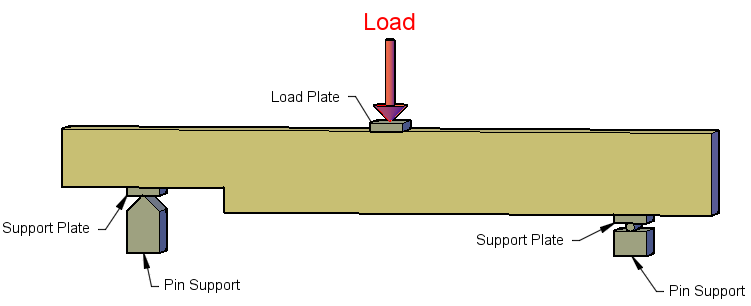
\includegraphics[scale=0.55]{Rectangular_Set_up}
	\end{center}
	\caption{Rectangular Member Test Set-Up}
	\label{fig:rect}
\end{figure}

\noindent
The supports were 600mm apart, from centre to centre, and the member was placed so it sat over the support at 100mm in from either end (100mm from notch corner). A 5mm x 40mm x 60mm steel plate was also placed at the centre of the beam and under the point load to distribute the load. The tests were set-up within a 1000 kN capacity Avery MTS machine, where the MTS applied a load at a constant rate. AS1720 specifies instantaneous load rating to be a rate at which the member fails within a time frame of 5mins. After some alteration, the load rate was set to 10kN applied load per minute to comply with AS1720. 


\noindent
The round members used were 800mm in length with a 100mm diameter, which was design to maintain a similar moment of inertia with the rectangular member. The notch was cut to a depth of 25mm, which was chosen to stay within Department of Transport and Main Road's maximum limitations of 25\% depth loss. These members were sawn so their grain profile was radial. 

\vspace*{\baselineskip}

\noindent
The same set-up was used for the round specimens as used for the rectangular; with a simply supported, 3 point load set up, 600mm effective length between supports, and the specimen supported 100mm in from either end. The same MTS machine was used at the same loading rate applied, for ease of later comparison with the rectangular specimen results. This set-up can be seen in Figure \ref{fig:round}.


\begin{figure}[h]
	\begin{center}
		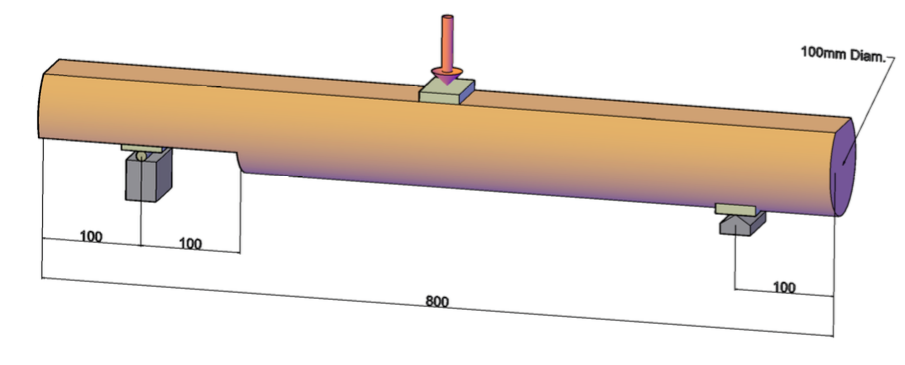
\includegraphics[scale=0.55]{Circular_Setup}
	\end{center}
	\caption{Round Member Test Set-Up}
	\label{fig:round}
\end{figure}
\pagebreak

\noindent
A rounded 5mm thick by 40mm wide metal loading plate was made, curving half of the members circumference, with a 3mm x 40mm x 300mm long, straight pieced of metal welded to one side to support the LVDT. This plate can be seen in Figure \ref{fig:RoundPlate}. 

\begin{figure}[h]
	\begin{center}
		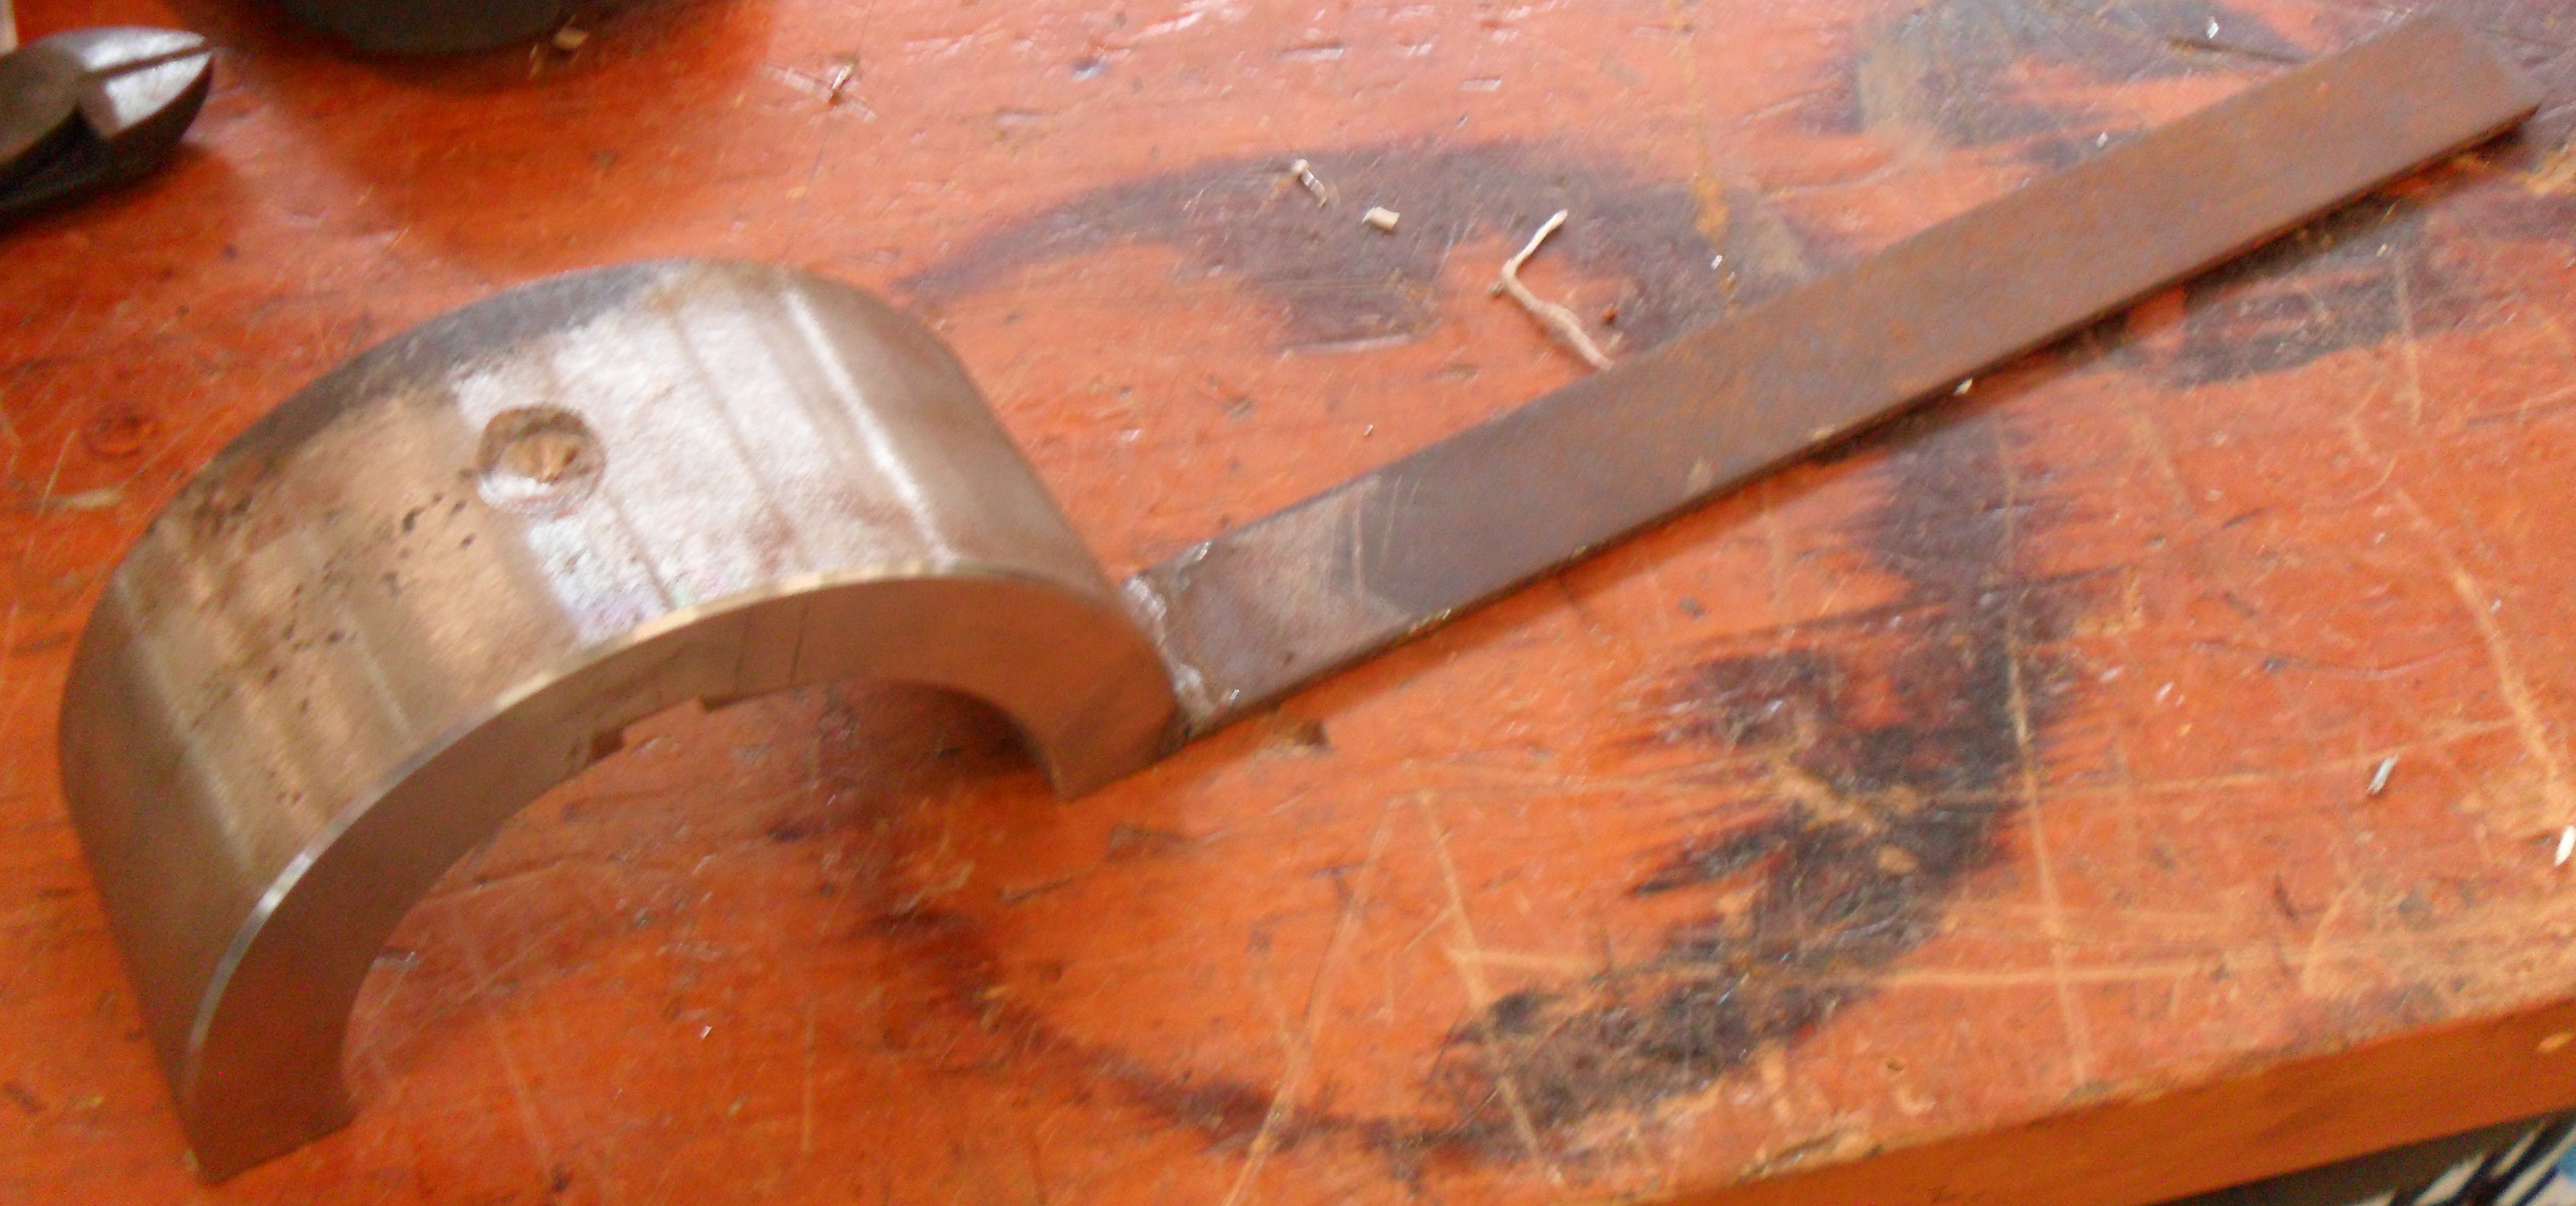
\includegraphics[scale=0.1]{Round_Plate}
	\end{center}
	\caption{Loading and LVDT Plate for Round Specimen}
	\label{fig:RoundPlate}
\end{figure}

\vspace*{\baselineskip}

\noindent
\textbf{Specimen Documentation}\par
\noindent
Before any testing was undertaken, the specimens were required to be documented in great detail, to account for any inaccuracies or defect interference with experimental results. Firstly, the length, width, depth, average diameter, notch length, notch depth and mass were measured and recorded. After the mass and all required dimensions were taken, the specimen was carefully checked for defects and imperfections (i.e. knots, rot, cracks etc.), which were measured, photographed and documented. This process was repeated for all 24 specimens. 

\vspace*{\baselineskip}

\noindent
\textbf{Specimen Strain Gauge Implementation}\par
\noindent
The locations for the expected maximum loading effects on the beam were determined using ANSYS modelling and strain gauges were used on all specimens to measure strains in these locations, within the constraints of the test set-up.

\begin{figure}[h]
	\begin{center}
		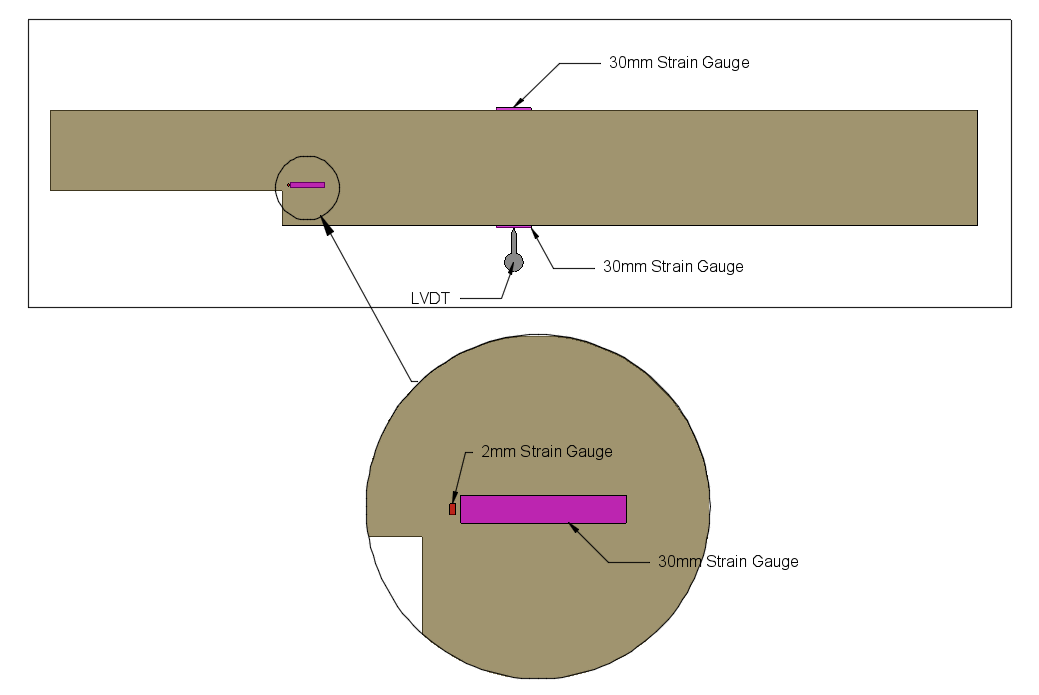
\includegraphics[scale=0.4]{Gauge_Set_Up}
	\end{center}
	\caption{Strain Gauge and LVDT Layout}
	\label{fig:Gauge}
\end{figure}

\noindent
As shown in Figure \ref{fig:Gauge}, a 2mm (FLA2--11--3L) strain gauge will be placed 5mm vertically and horizontally from the notch corner with a 30mm (PFL--30--11--3L) strain gauge directly next to it. This arrangement will be mirrored on both sides of the notch, and a 30mm strain gauge will be placed centrally on the top and bottom of the centre of the beam. These strains will be used to determine an overall stress profile for the notch and at the centre of the beam and to gain a better understanding of how notches reacted to applied loads. 

\vspace*{\baselineskip}

\noindent
To prepare for the strain gauges to be adhered to a specimen, each specimen was measured and marked on their top and bottom faces at the centre of the beam, and at the notch corner, to show the intended gauge placements. After this, the 30mm strain gauge was centrally placed on the marking in the middle of the top and bottom face of the beam using epoxy adhesive, running along the grain. The 2mm and 30mm strain gauges were then placed near the notch corner as marked on either side of the specimen. If the wires from a strain gauge were touching, they separated using duct tape. The strain gauges were arranged and properly attached to specimens between experiments.

\vspace*{\baselineskip}

\noindent
\textbf{LVDT Implementation}\par
\noindent
For the rectangular specimens, a 20cm long, 2cm wide and 5mm thick piece of plywood was attached to the specimen and mid-span using super glue. Once it was dry and secured, a 50mm LDVT was magnetically attached to the MTS machine and placed directly above the piece of plywood. For the round specimens, a long metal plate was incorporated into the constructed curved loading plate, which levelly extruded from the centre of the beam to allow seating for the LVDT.

\vspace*{\baselineskip}

\noindent
\textbf{Camera Implementation}\par
\noindent
A 400fps camera was used to video the notch of each specimen during loading. The camera was connected to a magnetic lever arm which would magnetically attach to the MTS machine. This allowed the camera to be moved to the optimal position, to capture the notch failure, for each experiment.

\vspace*{\baselineskip}

\noindent
\textbf{Timber Specimen Test Set-Up}\par
\noindent
Once the strain gauges had been securely attached to a specimen, the specimen was ready to be set-up to undertake loading. To set-up the experiment, the timber specimen was placed upon the simply supported arrangement within the MTS machine. This arrangement consisted of the notched end supported by a pin support and un-notched end supported by a roller, as shown in Figure \ref{fig:set_up}.

\begin{figure}[h]
	\begin{center}
		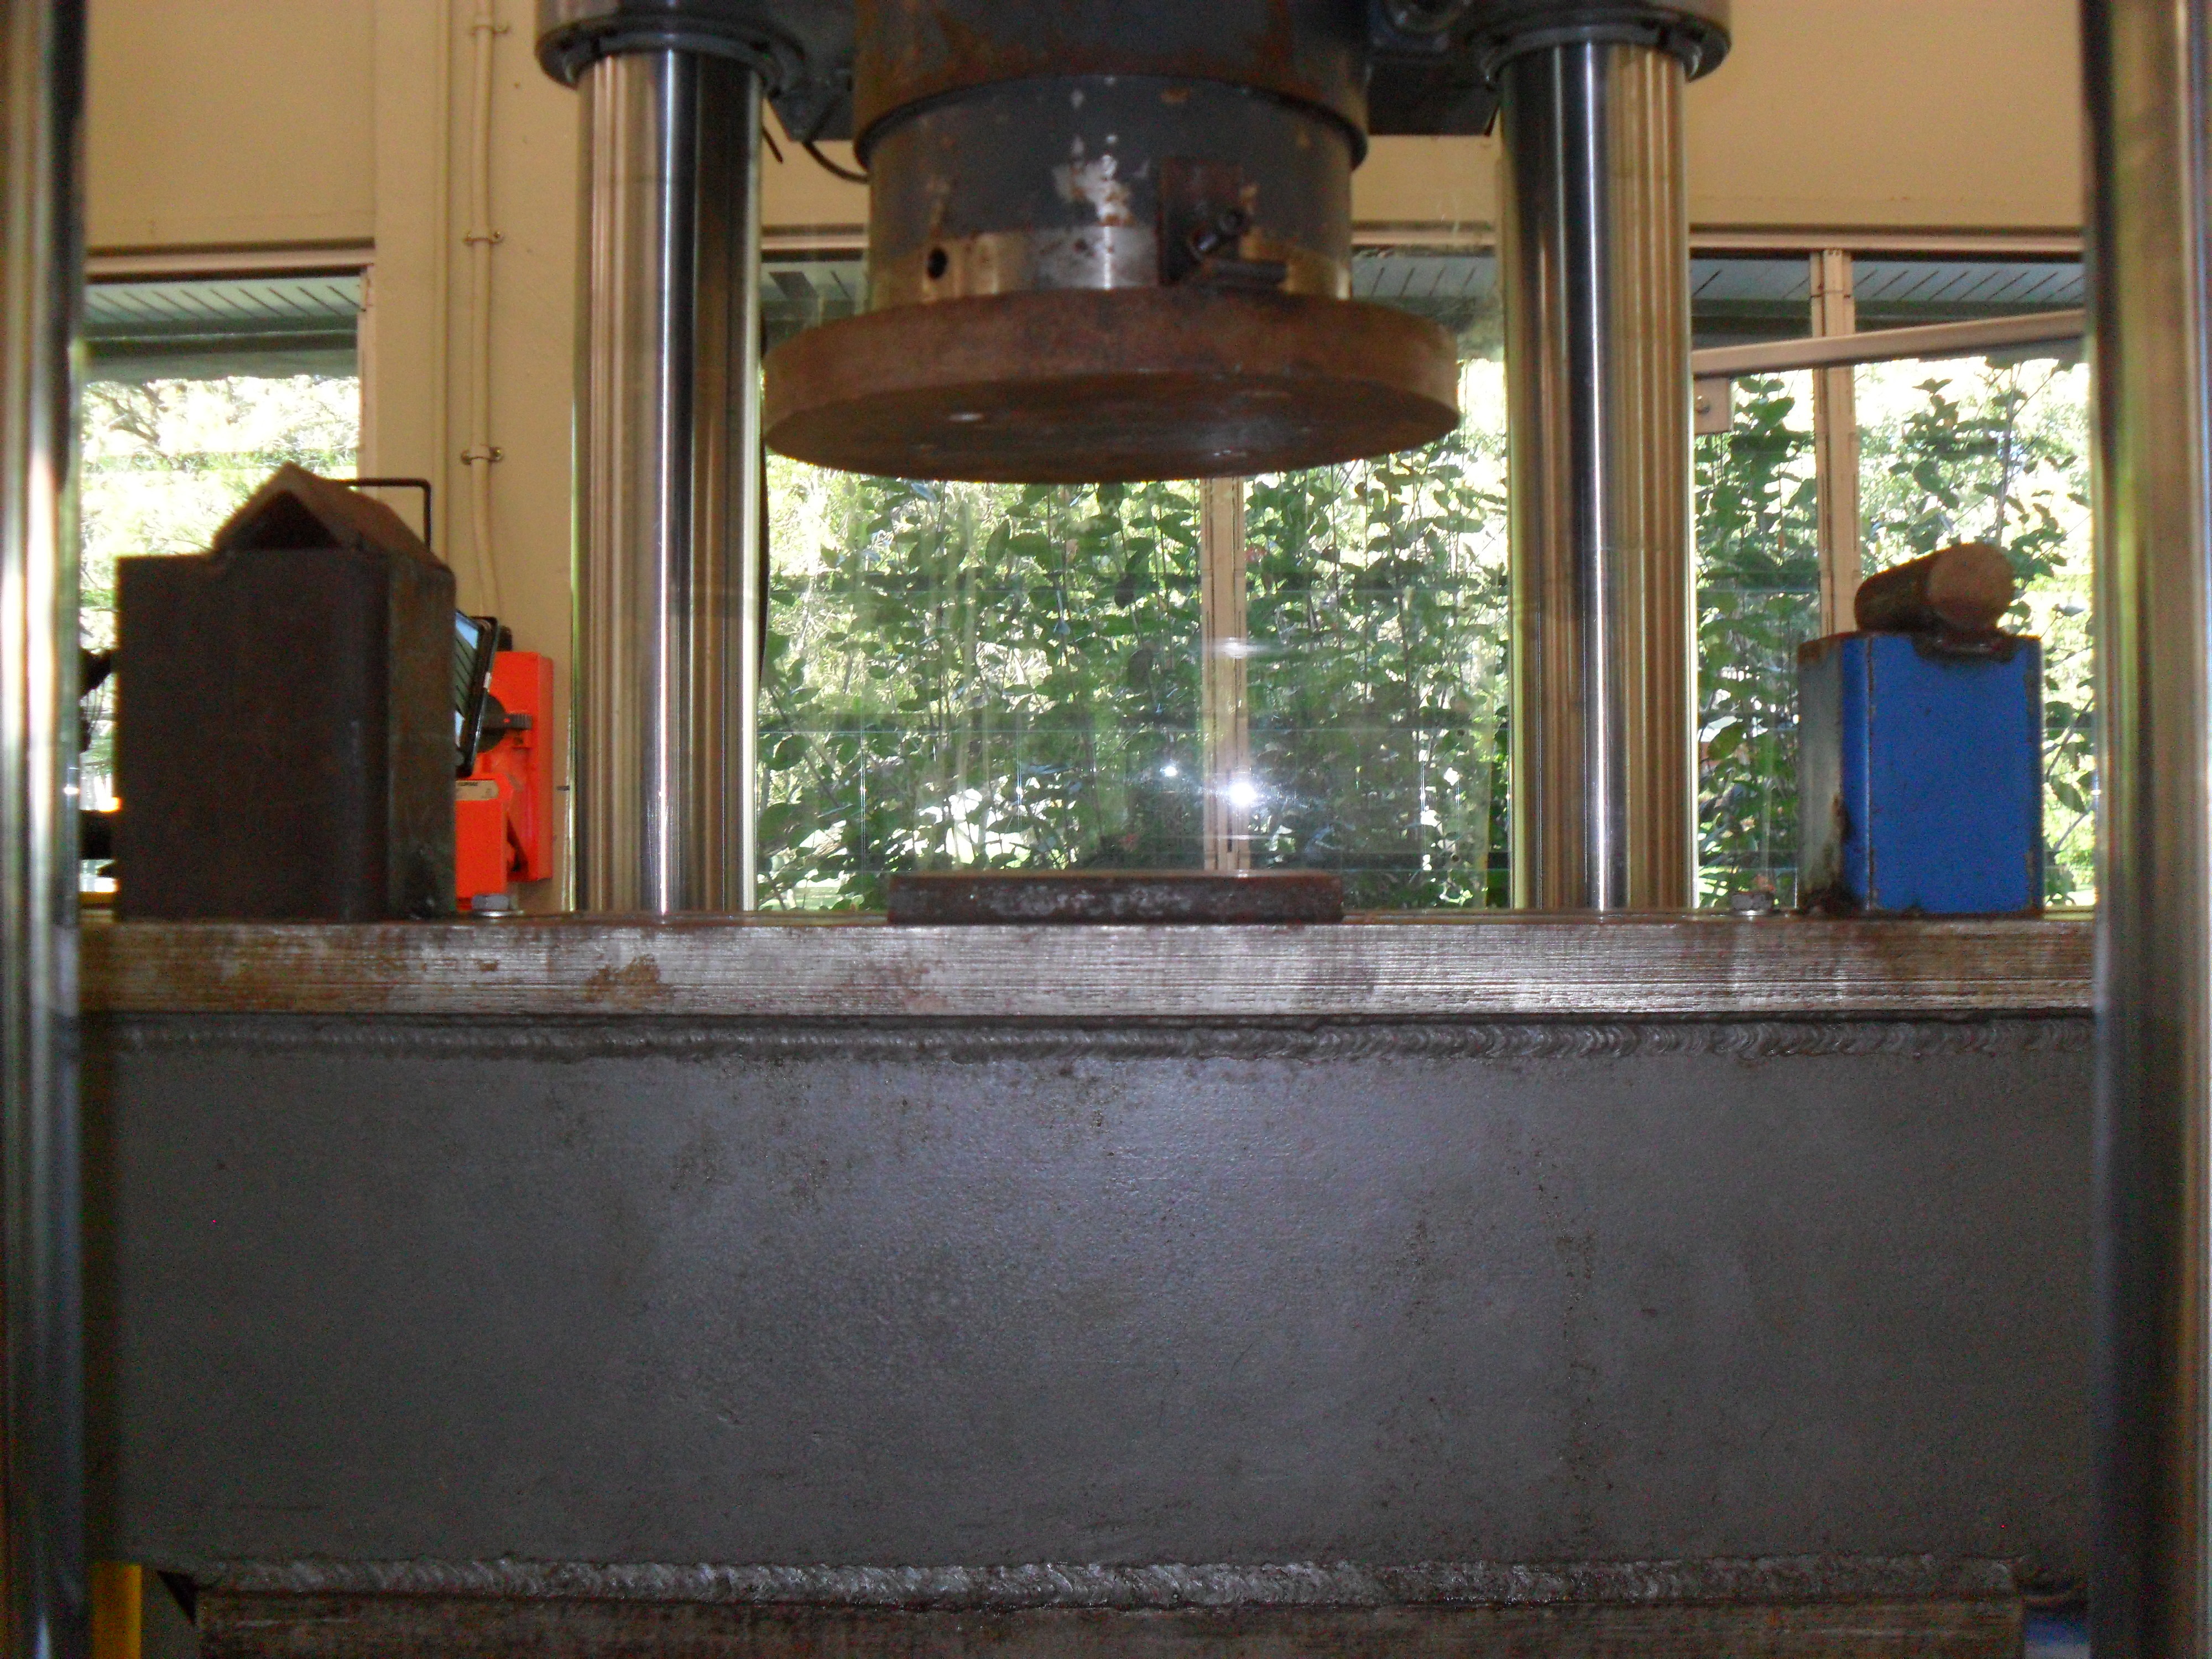
\includegraphics[scale=0.1]{MTS_Set-up}
	\end{center}
	\caption{Experimental Set-up in MTS Machine}
	\label{fig:set_up}
\end{figure}
\pagebreak

\noindent
The metal support plates were then slipped under the member to sit centrally above the two end supports, with extreme care taken to not pull on any strain gauges throughout the set-up. 

\vspace*{\baselineskip}

\noindent
\textbf{Data Logger Set Up}\par
\noindent
After the specimen experimental arrangement was complete, the strain gauges, LVDT and Load Cell were connected to the data logger. This was achieved by wiring 8 ports of the data logger with long wires that had alligator clips at the opposing ends.

\vspace*{\baselineskip}

\noindent
\textbf{Timber Specimen Testing}\par
\noindent
Once the specimen was correctly placed, set-up and all strain gauges and the LVDT was connected, the load cell was placed on top of the loading plate, a steel disc and a steel ball. A 5mm x 100mm x 100mm steel loading plate was then placed on top of the load cell, and the MTS load was lowered until it was just touching the top loading plate. Before we began loading, the data logger readings from the strain gauges, LVDT and load cell were checked to determine if all were properly connected and collecting data, the overall set-up can be seen in Figure \ref{fig:SETUP}.

\begin{figure}[h]
	\begin{center}
		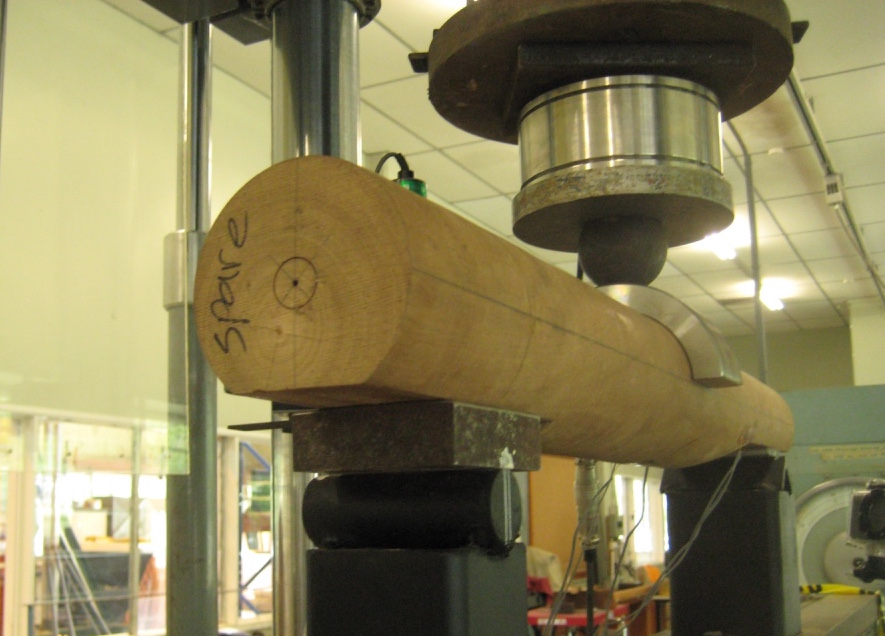
\includegraphics[scale=0.35]{SETUP}
	\end{center}
	\caption{Set-up of loading plates, metal ball and load cell in MTS Machine}
	\label{fig:SETUP}
\end{figure}
\pagebreak

\noindent
Finally, the data logger was zeroed, then a load was applied at a constant rate, by the MTS machine, until the specimen failed. 

\vspace*{\baselineskip}
\noindent
The steps described in the specimen strain gauge implementation, LVDT implementation, timber specimen test set-up, data logger set up and timber specimen testing were repeated for all 24 specimens. All tests were completed in the James Cook University structural engineering lab. 

\vspace*{\baselineskip}
\noindent
Overall, the data from the strain gauges, LVDT and load cell were collected to determine any trends and to compare between the two different sections. These results were used alongside the video footage of each experiment, to align points of cracking and failure with the data. 
\pagebreak

\subsubsection{Altering Notch Angles of Small Scale Members}
Three notch slopes were tested in this experiment; slopes 1:0, 1:2 and 1:4. These notch slopes were chosen as they are commonly used in timber bridging and have direct design methods in AS1720, which can be used for later comparison. The strains surrounding the notch and failure type were be observed to determine the critical notch angle. 

\begin{figure}[h]
	\begin{center}
		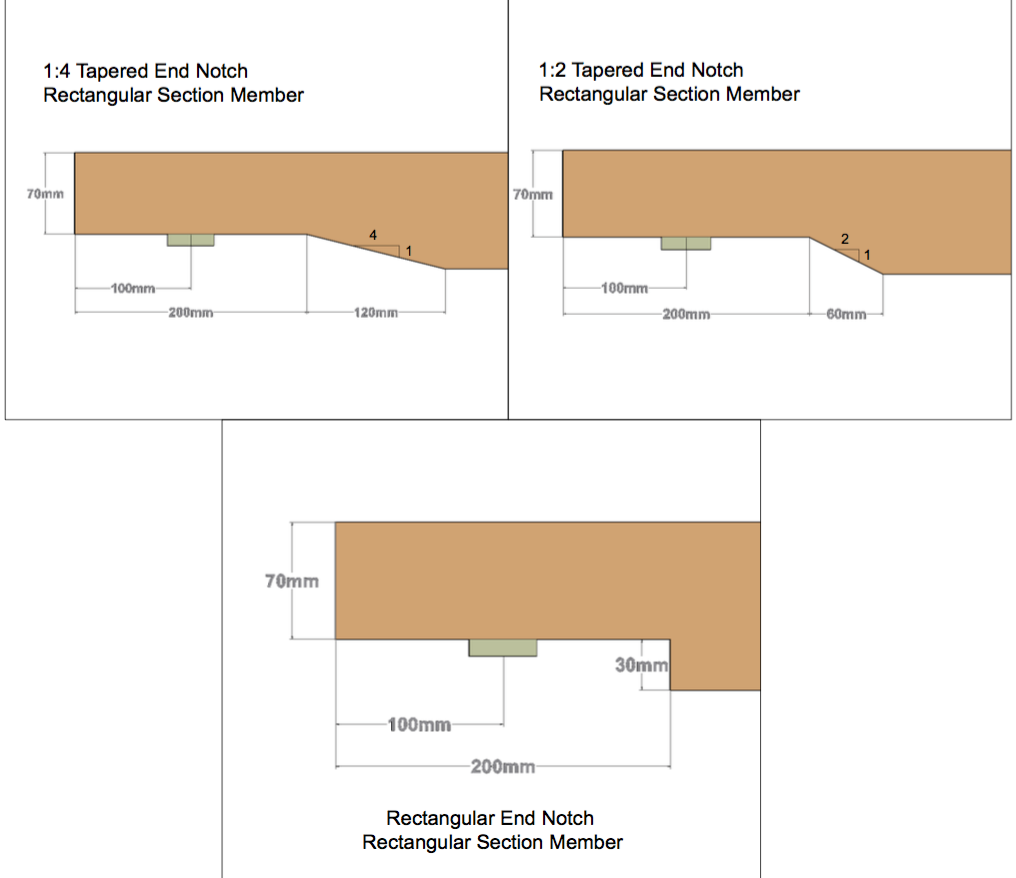
\includegraphics[scale=0.4]{Notch_Angles}
	\end{center}
	\caption{Notch Profiles for Rectangular Section Members}
	\label{fig:Rectangular2}
\end{figure}
\pagebreak

\noindent
A set of 4 specimens for each notch angle in both rectangular and circular section were tested, thus a total of 24 specimens are to were used. The notch layout for each test can be seen in Figures \ref{fig:Rectangular2} and \ref{fig:Circular}.
\vspace*{\baselineskip}
\begin{figure}[h]
	\begin{center}
		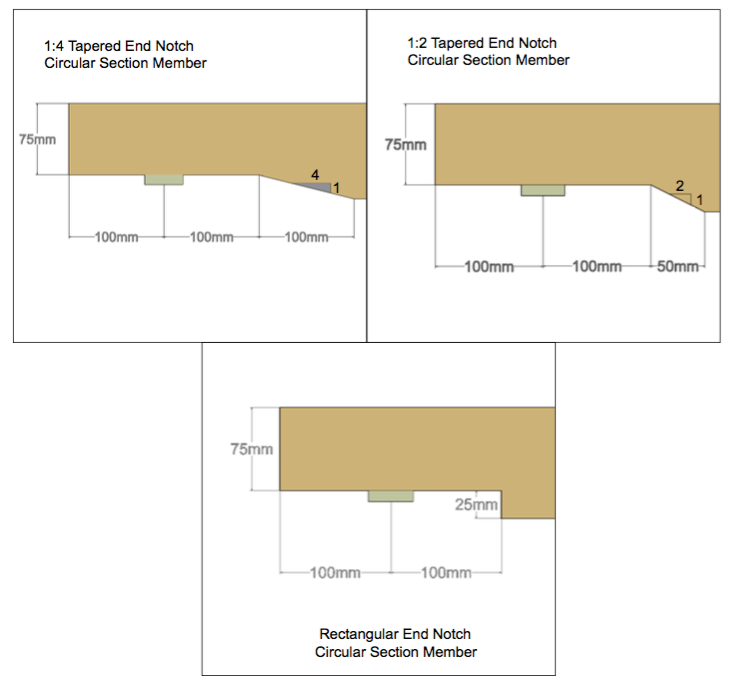
\includegraphics[scale=0.55]{Circular_Notch_Angles}
	\end{center}
	\caption{Notch Profiles for Circular Section Members}
	\label{fig:Circular}
\end{figure}

\noindent
Table 3 shows the set experimental parameters for each section shape and notch profile. As it can be seen, the moment of inertia between the two section is approximately equal, with a difference of $0.09 x 10^{6} mm^{4}$.

\pagebreak
\captionof{table}{Experimental Parameters}

\begin{center}
	\begin{tabularx}{\textwidth}{|>{\centering}X|>{\centering}X|>{\centering}X|>{\centering}X|>{\centering}X|>{\centering}X|>{\centering}X|>{\centering}X|} 
		\hline
	    \multicolumn{8}{|c|}{\textbf{Rectangular Section}} \\
		\hline
	%	\cline{2-3}
		
		\textbf{Notch Profile} & \textbf{Notch Angle Slope} & \textbf{Member Depth (mm)} & \textbf{Width (mm)} & \textbf{Notch Depth (mm)} & \textbf{Total Section Area ($mm^{2}$)} & \textbf{Area Above Notch Corner ($mm^{2}$)} & \textbf{Moment of Inertia ($10^{3} mm^{4}$)} \tabularnewline [0.5ex] 
		\hline
		1 & 1:0 & 100 & 60 & 30 & 6000 & 4200 & 5000 \tabularnewline [0.5ex]
		\hline
		2 & 1:2 & 100 & 60 & 30 & 6000 & 4200 & 5000 \tabularnewline [0.5ex]
		\hline
		3 & 1:4 & 100 & 60 & 30 & 6000 & 4200 & 5000 \tabularnewline [0.5ex]
		\hline
	   
	    \multicolumn{8}{|c|}{\textbf{Circular Section}} \\
	    \hline
	    
	    \textbf{Notch Profile} & \textbf{Notch Angle Slope} & 
	    \multicolumn{2}{c|}{\textbf{Diameter (mm)}}
	    & \textbf{Notch Depth (mm)} & \textbf{Total Section Area ($mm^{2}$)} & \textbf{Area Over Notch Corner ($mm^{2}$)} & \textbf{Moment of Inertia ($10^{3} mm^{4}$)} \tabularnewline [0.5ex] 
	    \hline
	    1 & 1:0 & \multicolumn{2}{c|}{100} & 25 & 7850 & 6320 & 4910 \tabularnewline [0.5ex]
	    \hline
	    2 & 1:2 & \multicolumn{2}{c|}{100} & 25 & 7850 & 6320 & 4910 \tabularnewline [0.5ex]
	    \hline
	    3 & 1:4 & \multicolumn{2}{c|}{100} & 25 & 7850 & 6320 & 4910 \tabularnewline [0.5ex]
	    \hline
	\end{tabularx}
\end{center}

\vspace*{\baselineskip}

\subsection{Material Properties}
\noindent \textbf{Timber Properties}\par
\noindent
The timber used for testing was spotted gum (corymbia maculata) timber, as it a hardwood that is commonly used in Queensland bridges that are currently being utilised. The properties and characteristics of spotted gum timber are given in Table \ref{tab:spotty} \cite{elsener_material_2014,hopewell_spotted_2004}. All specimens will be unseasoned and green (have a water content greater than 12\%), and all timber was sourced from Grays Sawmill in Proserpine, Queensland.

\pagebreak

\captionof{table}{Properties of Spotted Gum (Corymbia Maculata) \cite{elsener_material_2014,hopewell_spotted_2004}}
\label{tab:spotty}

\begin{center}
	\begin{tabularx}{\textwidth}{|>{\centering}X|>{\centering}X|>{\centering}X|>{\centering}X|>{\centering}X|}	
		\hline 
		
		\multicolumn{2}{|c|}{\textbf{Properties}} & \textbf{Moisture Content 12\%} & \textbf{Green (MC $\textgreater$ 12\%)}  & \textbf{Dry (MC $\textless$ 12\%)} \tabularnewline  [0.5ex]
		\hline
		
		\multirow{3}{*}{\parbox{2.5cm}{\centering Modulus of Rupture MOR (MPa)}}& \textit{Longitudinal} & 141.1 & 99 & 150 \tabularnewline  [0.5ex] 
		\cline{2-5}
		& \textit{Radial} & 19.5 &  &  \tabularnewline [0.5ex] 
		\cline{2-5}
		& \textit{Tangential} & 14.9 &  &  \tabularnewline [0.5ex] 
		\hline
		
		\multirow{3}{*}{\parbox{2.5cm}{\centering Modulus of Elasticity MOE (MPa)}} & \textit{Longitudinal} & 26174 & 18000 & 23000 \tabularnewline [0.5ex] 
		\cline{2-5}
		& \textit{Radial} & 2405 & 1531 &  \tabularnewline [0.5ex] 
		\cline{2-5}
		& \textit{Tangential} & 1499 & 665 &  \tabularnewline [0.5ex] 
		\hline
		
		\multirow{3}{*}{\parbox{2.5cm}{\centering Shear Modulus G (MPa)}}& \textit{Long - Rad} & 1736 &  &  \tabularnewline [0.5ex] 
		\cline{2-5}
		& \textit{Rad - Tang} & 840 &  &  \tabularnewline [0.5ex] 
		\cline{2-5}
		& \textit{Long - Tang} & 1530 &  &  \tabularnewline [0.5ex] 
		\hline
		
		\multirow{6}{*}{\parbox{2.5cm}{\centering Poisson's Ratio $\nu$}}& \textit{Long - Rad} & 0.49 &  &  \tabularnewline [0.5ex] 
		\cline{2-5}
		& \textit{Long - Tang} & 0.550 &  &  \tabularnewline [0.5ex] 
		\cline{2-5}
		& \textit{Rad - Tang} & 0.660 &  &  \tabularnewline [0.5ex] 
		\cline{2-5}
		& \textit{Rad - Long} & 0.045 &  &  \tabularnewline [0.5ex] 
		\cline{2-5}
		& \textit{Tang - Rad} & 0.480 &  &  \tabularnewline [0.5ex] 
		\cline{2-5}
		& \textit{Tang - Long} & 0.047 &  &  \tabularnewline [0.5ex] 
		\hline
		
		
		\multicolumn{2}{|c|}{Bending Strength (MPa)}& 142 &  &   \tabularnewline [0.5ex] 
		\hline
		
		\multicolumn{2}{|c|}{Compressive Strength (MPa)}& 76 &  &   \tabularnewline [0.5ex] 
		\hline
		
		\multicolumn{2}{|c|}{Tensile Strength (MPa)}& 159 &  &   \tabularnewline [0.5ex] 
		\hline
		
		\multicolumn{2}{|c|}{Density ($kg/m^{3}$)}& 1060 & 1150 & 1100  \tabularnewline [0.5ex] 
		\hline
		
		\multicolumn{2}{|c|}{Strength Group}&  & S2 & SD2  \tabularnewline [0.5ex] 
		\hline
		
		\multicolumn{2}{|c|}{F-Grade}&  & F14 & F22  \tabularnewline [0.5ex] 
		\hline
		
	\end{tabularx}
\end{center}

\subsection{Finite Element Analysis}
Finite element analysis (FEA) was completed on ANSYS V17.0 to compare theoretical effects of the experiments with actual results, as well as allow the observation of experimental effects on large scale models. 

\vspace*{\baselineskip}

\noindent
The properties used for the FEA modelling in ANSYS can  be seen in Figure \ref{fig:Properties} below.
\begin{figure}[h]
	\begin{center}
		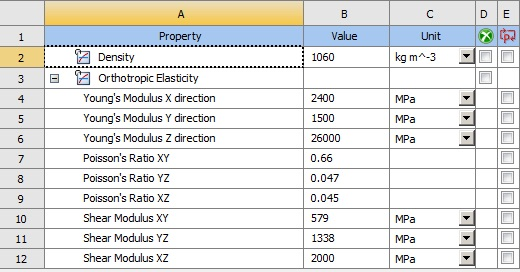
\includegraphics[scale=0.8]{Ansys_Properties}
	\end{center}
	\caption{Properties Used for ANSYS Simulation}
	\label{fig:Properties}
\end{figure}
\pagebreak
\vspace*{\baselineskip}
\pagebreak

\section{Results and Discussion}

\subsection{Rectangular Specimens}
\subsubsection{Loading Rates}
The loading rates used to load the rectangular specimens can be seen in Figure \ref{fig:Rect_load}. It can be seen that the load rate was constant throughout loading all specimens, at a load rate of 10kN per minute. 

\begin{figure}[h]
	\begin{center}
		\fbox{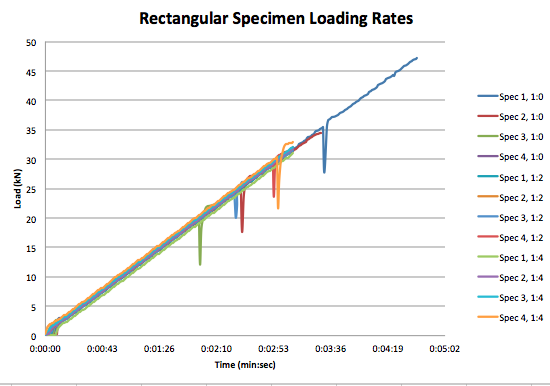
\includegraphics[scale=0.7]{Rect_load}}
	\end{center}
	\caption{Load rates for rectangular specimens}
	\label{fig:Rect_load}
\end{figure}

\noindent
It can also be seen from Figure \ref{fig:Rect_load} that every specimen experienced an extreme drop in load at some point throughout the experiment. The reason for this was at first presumed to be due to the notch crack initiating at this point. However, when compared to the actual loads at which the notch crack initiates, see Table \ref{tab:rect_Capac}, the drop appears to take place at a higher load. Therefore, it is presumed that the extreme decrease in load is the point at which the notch crack fully propagates passed the centre of the beam. This theory seems plausible as when the crack fully propagates, the member is essentially changing section, as the only part of the member taking the load, would be the remaining section above the crack, thus the reason for the sudden jump in load.  

\subsubsection{Failure Modes}
Table \ref{tab:Rect_Fail_Type} shows the water content and initial failure type of each specimen. From this is can be seen that the notch corner cracked on every specimen before ultimate failure occurred.

\vspace*{\baselineskip}

\captionof{table}{Rectangular Specimen Water Contents and Initial Failure Locations}
\begin{center}
	\begin{tabular}{|c|c|c|c|} 
		\hline
		
		\textbf{Notch Angle Slope} & \textbf{Specimen No.} & \textbf{Water Content (\%)} & \textbf{Location of Initial Failure}\\ [0.5ex]
		\hline
		
		1:0 & 1 &  & Cracked at notch corner \\ [0.5ex]
		\hline
		1:0 & 2 &  & Cracked at notch corner \\ [0.5ex]
		\hline
		1:0 & 3 &  & Cracked at notch corner \\ [0.5ex]
		\hline
		1:0 & 4 & 19 & Cracked at notch corner \\ [0.5ex]
		\hline
		
		1:2 & 1 & 14 & Cracked at notch corner \\ [0.5ex]
		\hline
		1:2 & 2 & 16 & Cracked at notch corner \\ [0.5ex]
		\hline
		1:2 & 3 & 16 & Cracked at notch corner \\ [0.5ex]
		\hline
		1:2 & 4 & 13 & Cracked at notch corner \\ [0.5ex]
		\hline
		
		1:4 & 1 & 19 & Cracked at notch corner \\ [0.5ex]
		\hline
		1:4 & 2 & 15 & Cracked at notch corner \\ [0.5ex]
		\hline
		1:4 & 3 & 18 & Cracked at notch corner \\ [0.5ex]
		\hline
		1:4 & 4 & 18 & Cracked at notch corner \\ [0.5ex]
		\hline
	\end{tabular}
	\label{tab:Rect_Fail_Type}
\end{center}

\vspace*{\baselineskip}
\noindent
It should be noted that the water contents for rectangular specimens 1, 2 and 3 of 1:0 notch were unable to be taken due to lack of required equipment.

\vspace*{\baselineskip}

\noindent
Throughout all rectangular experiments, there was a definite pattern in the types of failure that occurred; first a crack initiated from the notch corner, which propagated just passed the centre of the beam, then ultimate failure occurred. The crack would initiate by first opening perpendicular to the grain at the notch corner (notch failure mode 1), due to excessive tensile forces, which can be seen in Figure \ref{fig:Rect_Crack}. 

\begin{figure}[h]
	\begin{center}
		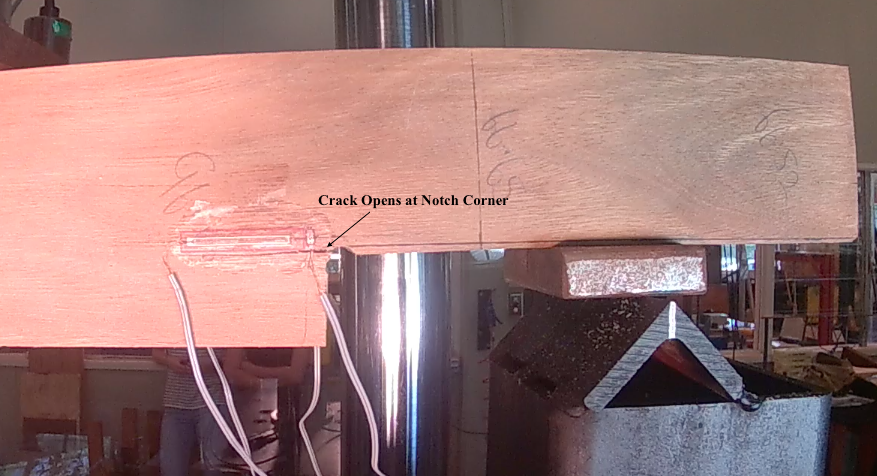
\includegraphics[scale=0.5]{Rect_Crack_Open}
	\end{center}
	\caption{Specimen 4 notch 1:0, notch crack opening}
	\label{fig:Rect_Crack}
\end{figure}
\pagebreak
\noindent
Then the crack would shear through the member (notch failure mode 2) and propagate to just passed the centre of the beam, as can be seen in Figure \ref{fig:Rect_Prop}. It can also be seen in Figure \ref{fig:Rect_Prop} that the notch corner crack opened (failure mode 3), due to a combination of the tensile and shear forces, which began to occur after the crack initially sheared.  

\begin{figure}[h]
	\begin{center}
		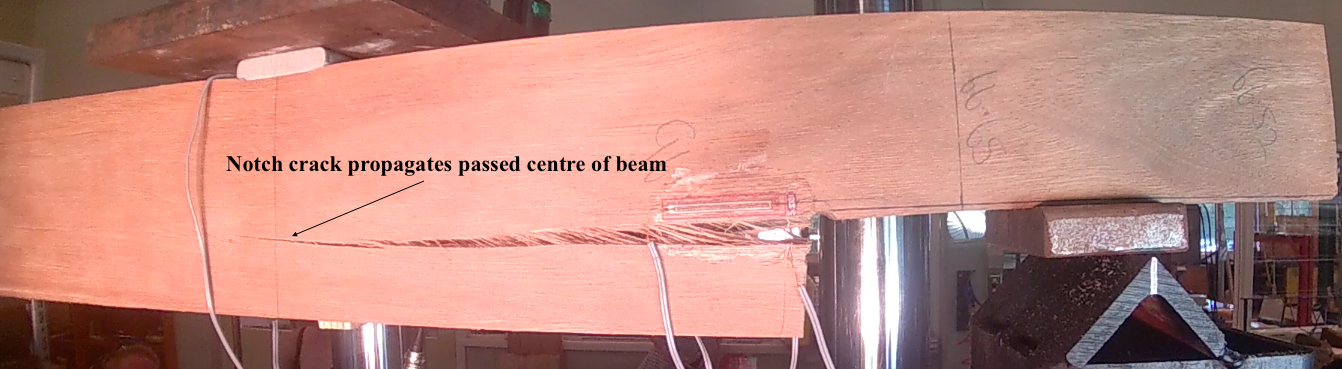
\includegraphics[scale=0.31]{Rect_propegate}
	\end{center}
	\caption{Specimen 4 notch 1:0, notch crack shearing and opening}
	\label{fig:Rect_Prop}
\end{figure}
\pagebreak

\noindent
After the notch crack had fully propagated passed the centre of the beam and began to open, the specimens then ultimately failed in shear as can been seen in Figure \ref{fig:Rect_Shear}. 

\begin{figure}[h]
	\begin{center}
		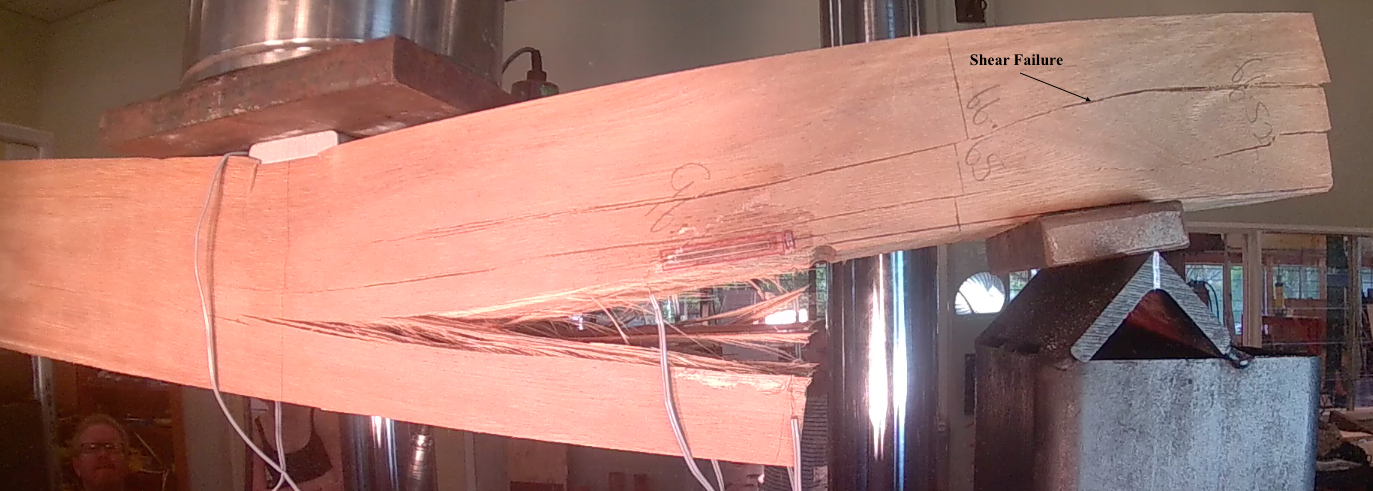
\includegraphics[scale=0.31]{Rect_Shear}
	\end{center}
	\caption{Specimen 4 notch 1:0, Shear Failure}
	\label{fig:Rect_Shear}
\end{figure}

\noindent
Almost immediately after ultimate shear failure occurred, the specimens then failed in flexure at the centre of the beam, as shown in Figure \ref{fig:Rect_Flex}. The overall succession of notch failure and ultimate failure occurred as expected; sequencing through the notch failure modes and ultimately failing in shear or flexure. 

\begin{figure}[h]
	\begin{center}
		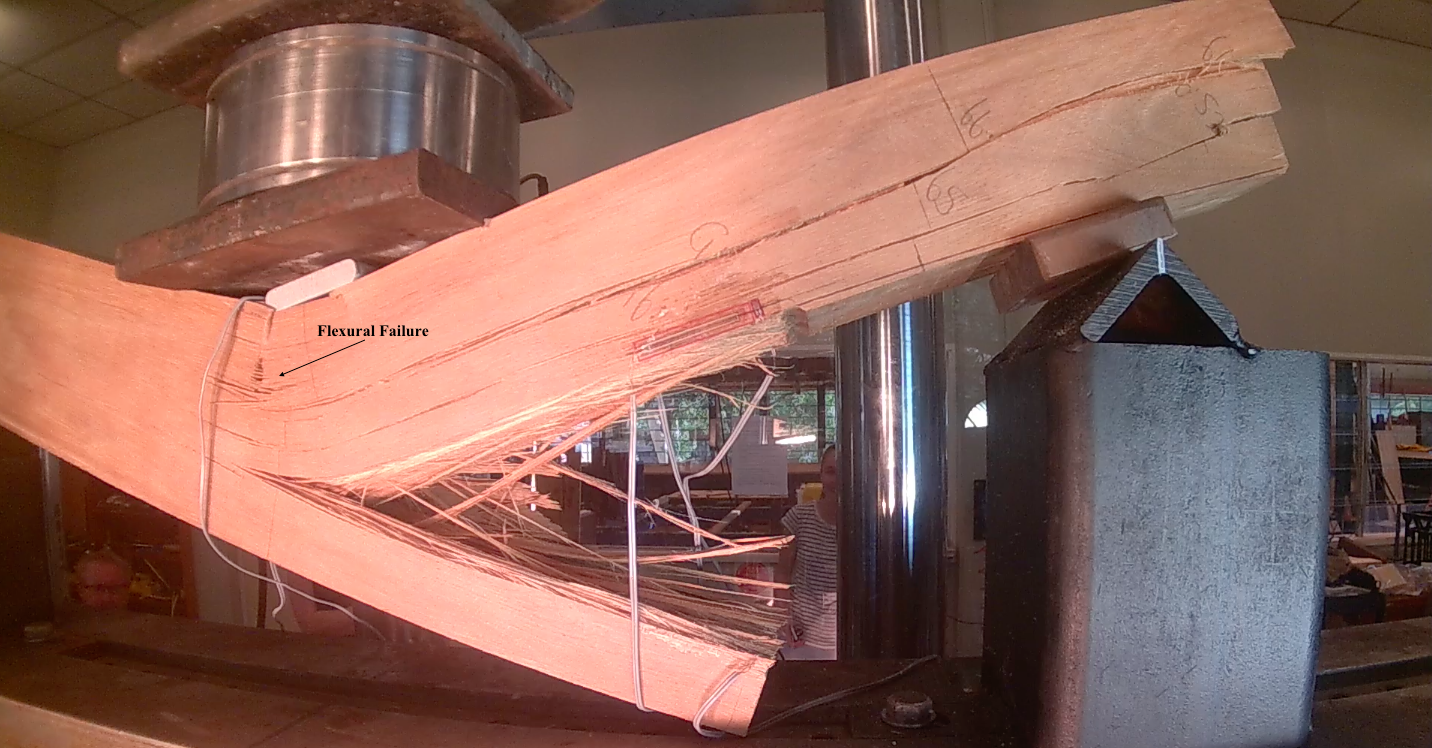
\includegraphics[scale=0.3]{Rect_Flexure}
	\end{center}
	\caption{Specimen 4 notch 1:0, Flexural Failure}
	\label{fig:Rect_Flex}
\end{figure}
\pagebreak

\noindent
All rectangular specimens ultimately failed in shear and then flexure, apart from specimen 2 of the 1:0 slope notch, which only failed in flexure, as shown in Figure \ref{fig:Spec_2}.

\begin{figure}[h]
	\begin{center}
		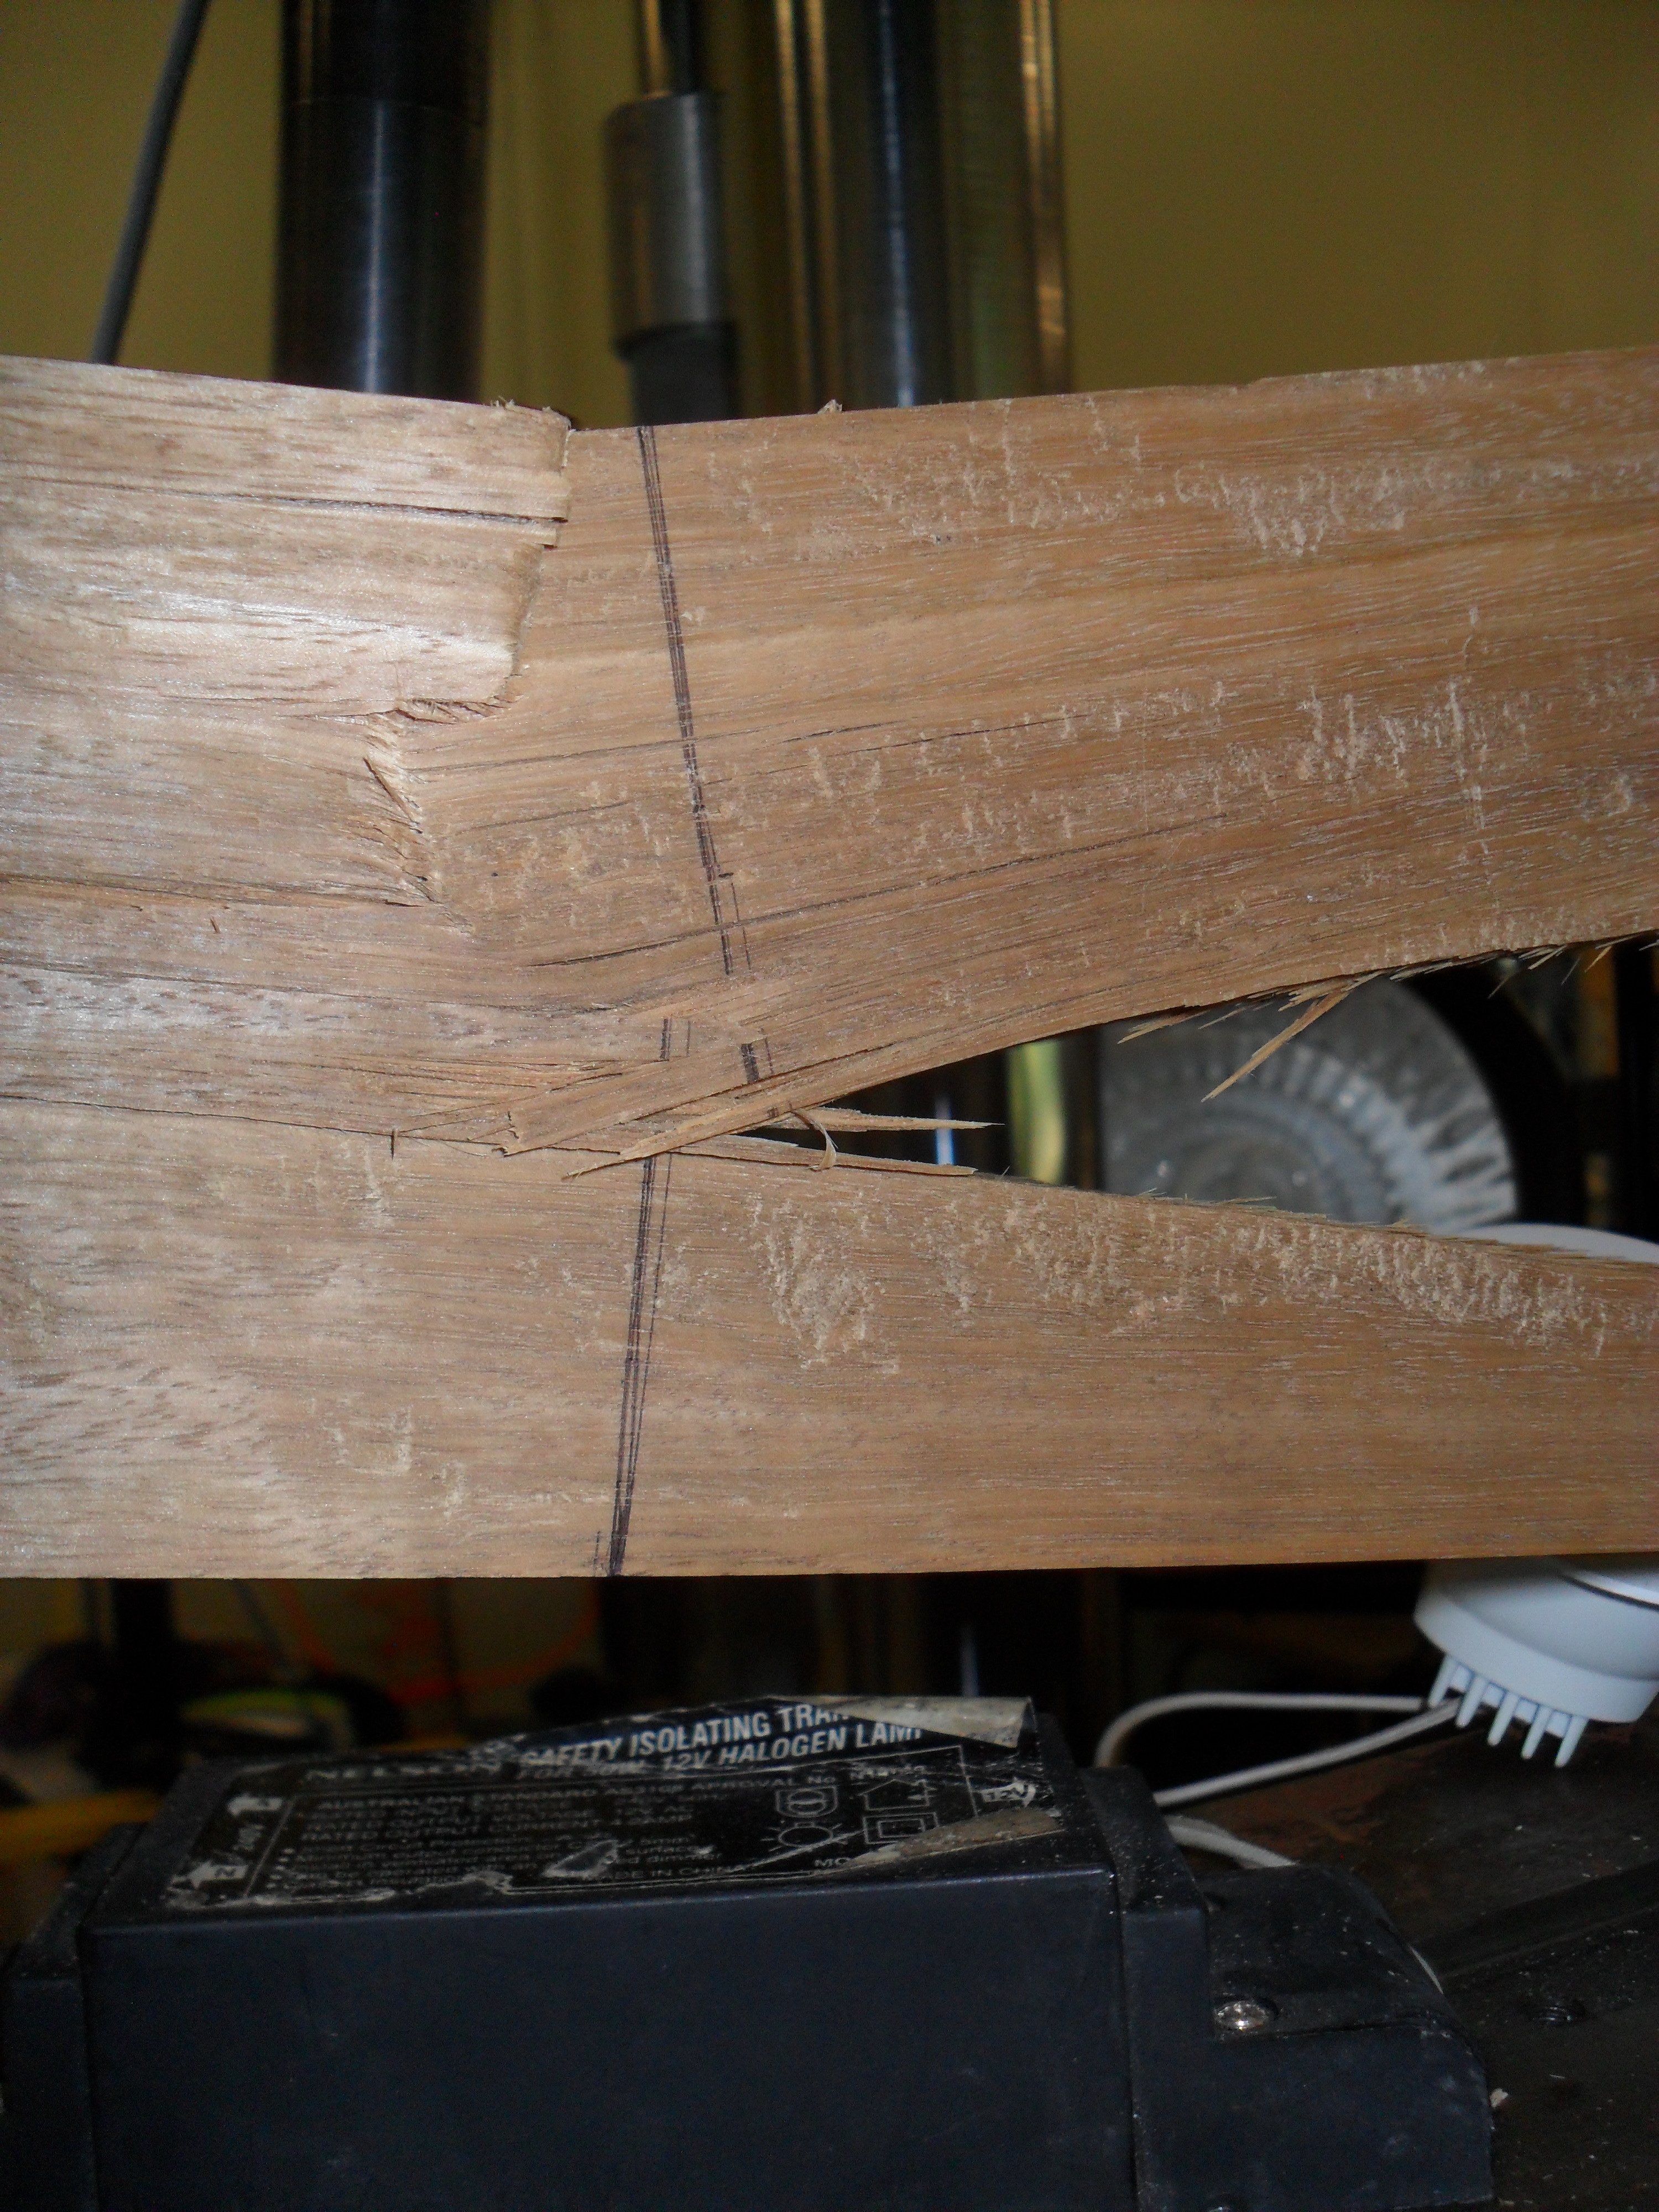
\includegraphics[scale=0.05]{Spec_2_flex}
		\includegraphics[scale=0.086]{Spec_2_Top}
	\end{center}
	\caption{Specimen 2 notch 1:0 failure; side view left, top view right}
	\label{fig:Spec_2}
\end{figure}

\noindent
The reason that this specimen did not fail in shear is overall unknown. There were no obvious defects present on or in the specimen on inspection. A possible reason would be the specimen had a very high water content at the centre of the beam, which significantly decreased it's flexural capacity in this region. The possible clause for this theory can be observed in Figure \ref{fig:Spec_2_wet}, where the specimen appears to be very wet in this specified area. However, the water content was not taken for this specific specimen, thus this theory can not be verified. 

\begin{figure}[h]
	\begin{center}
		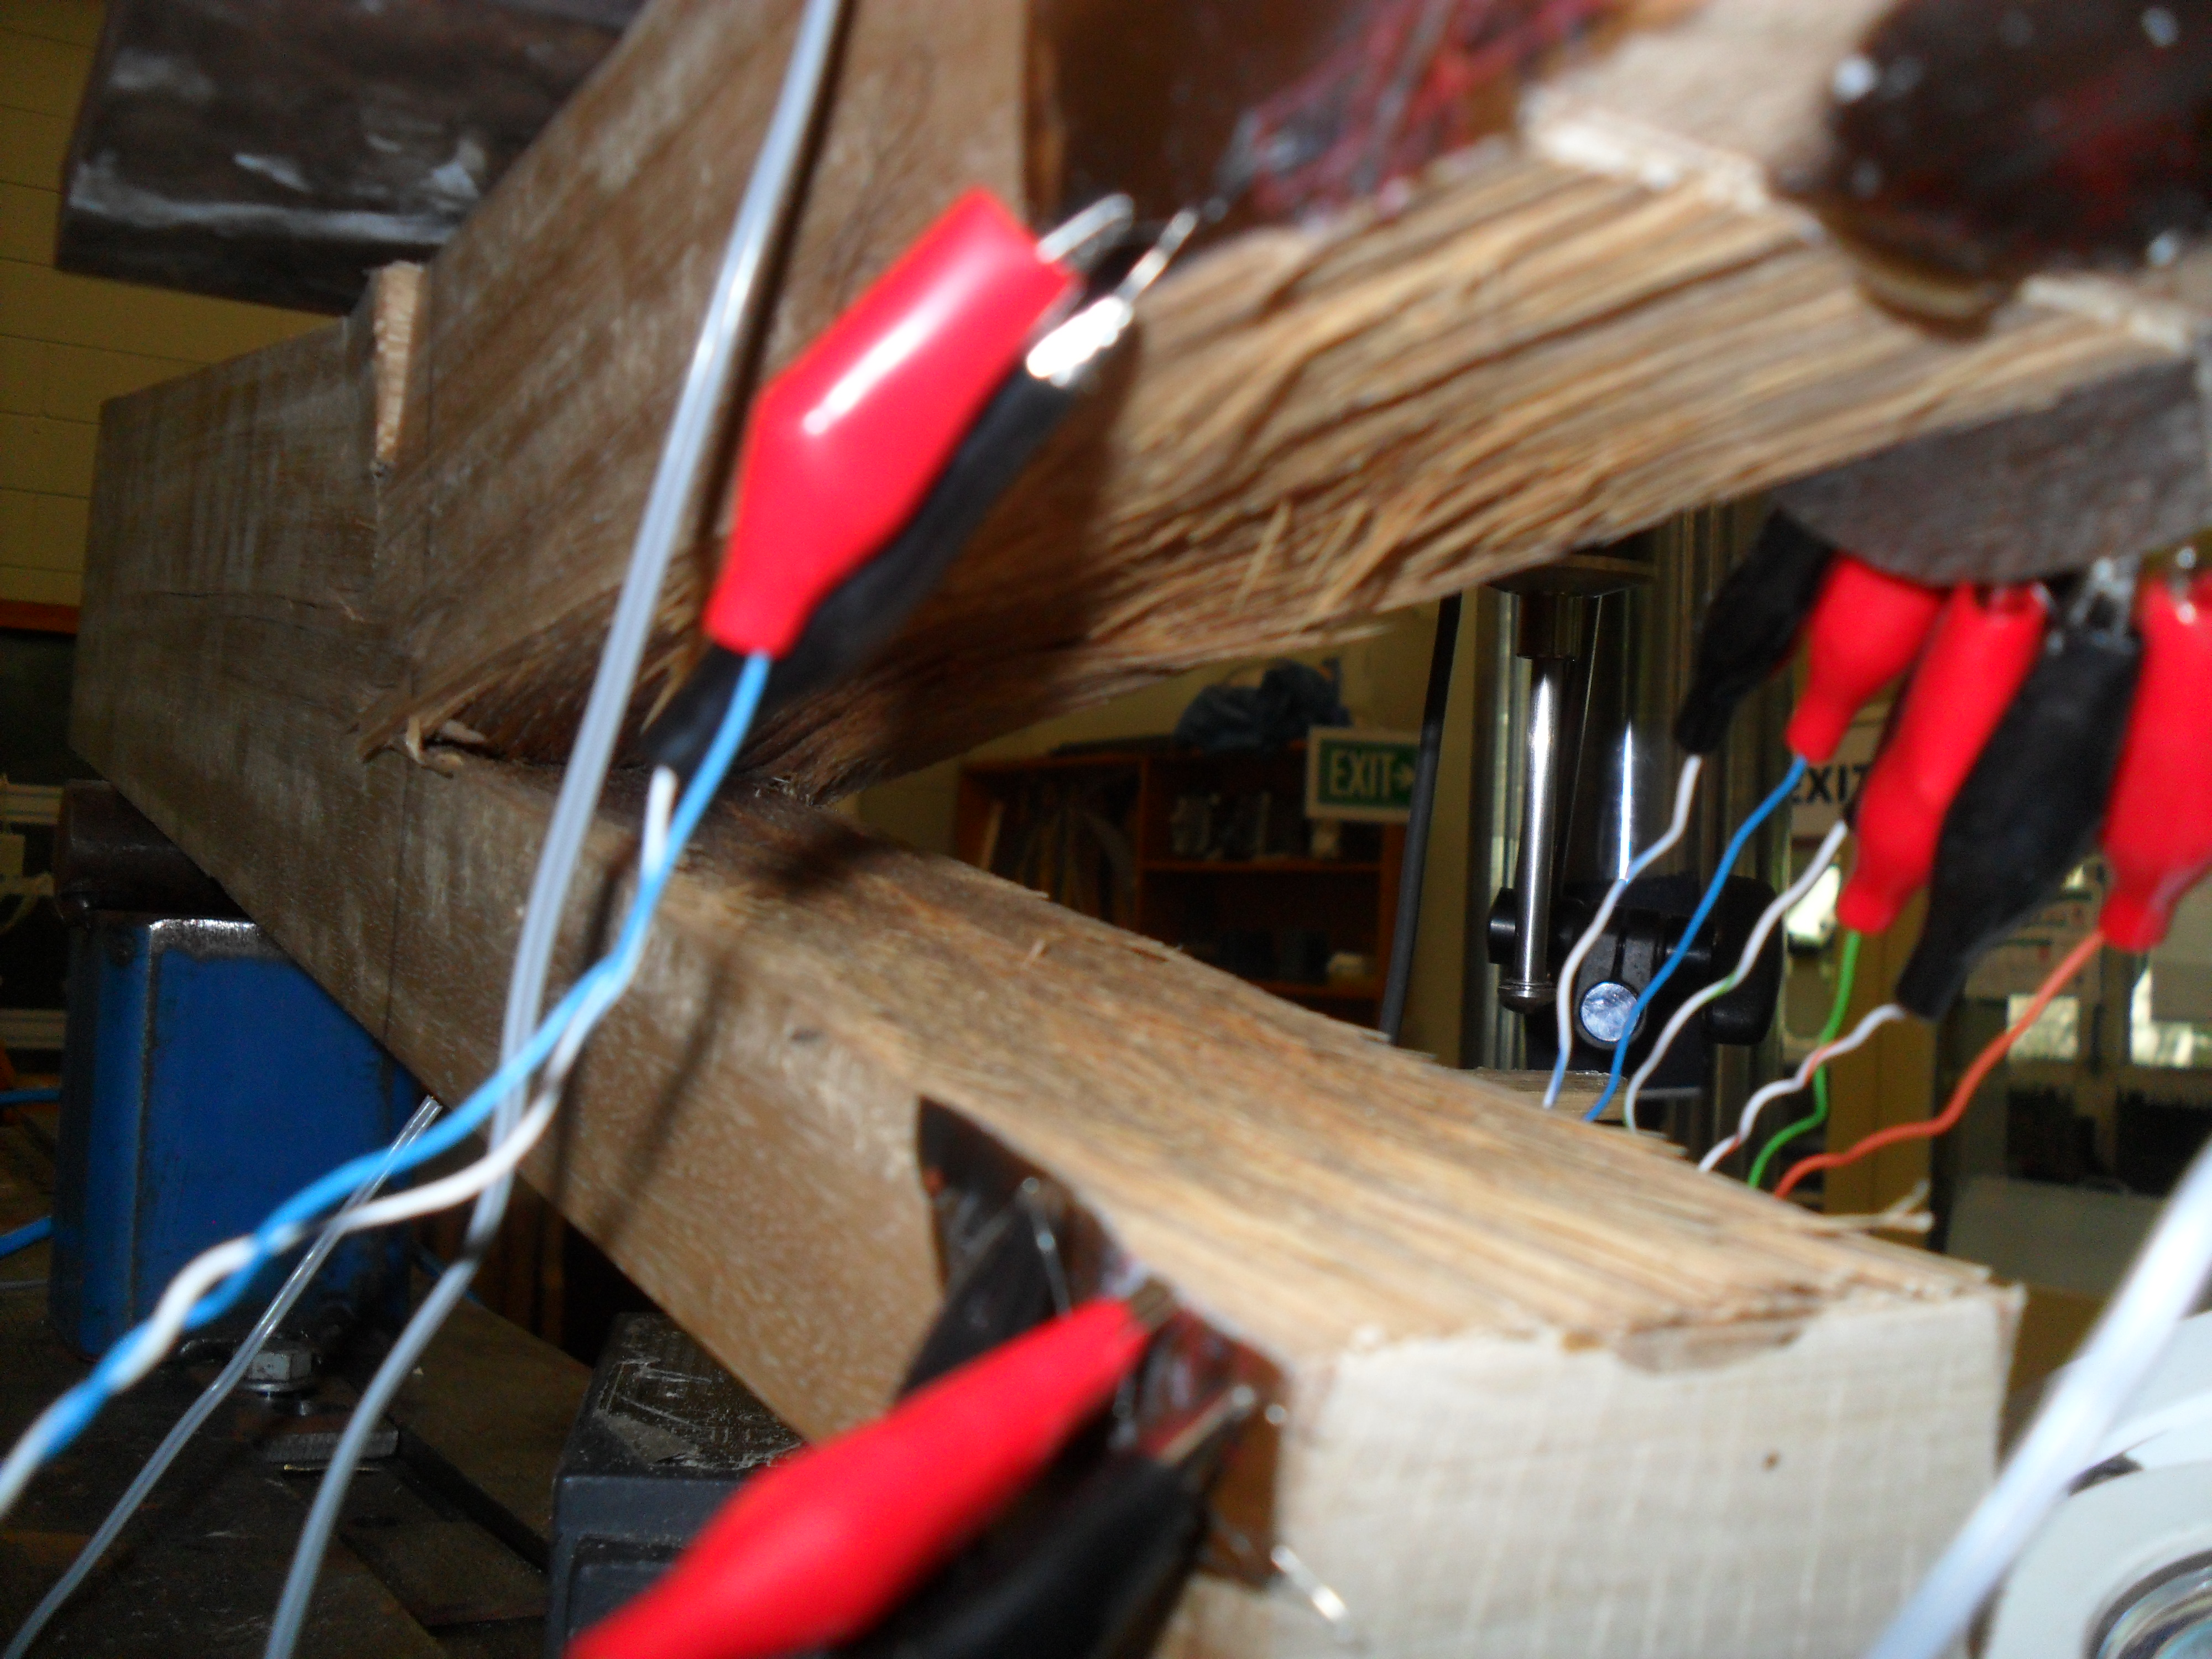
\includegraphics[scale=0.1]{Spec_2_wet}
	\end{center}
	\caption{Specimen 2 notch 1:0; inside centre of beam}
	\label{fig:Spec_2_wet}
\end{figure}

\noindent
The ultimate shear failure occurred roughly through the middle of the cross-section of one half of the beam. However the location alternated between, over the notch half and over the roller support half (opposing end to the notch), throughout the experiments. A summary of these locations can be seen in Table \ref{tab:Rect_Shear_Fail}.

\vspace*{\baselineskip}

\captionof{table}{Rectangular Specimen Water Contents and Initial Failure Locations}
\begin{center}
	\begin{tabularx}{\textwidth}{|>{\centering}X|>{\centering}X|>{\centering}X|} 
		\hline
		
		\textbf{Notch Angle Slope} & \textbf{Specimen No.} & \textbf{Shear Failure Location}\tabularnewline [0.5ex]
		\hline
		
		1:0 & 1 & Opposing end to the notch \tabularnewline [0.5ex]
		\hline
		1:0 & 2 & Opposing end to the notch \tabularnewline [0.5ex]
		\hline
		1:0 & 3 & Opposing end to the notch \tabularnewline [0.5ex]
		\hline
		1:0 & 4 & Over the notch \tabularnewline [0.5ex]
		\hline
		
		1:2 & 1 & Over the notch \tabularnewline [0.5ex]
		\hline
		1:2 & 2 & Over the notch \tabularnewline [0.5ex]
		\hline
		1:2 & 3 & Over the notch \tabularnewline [0.5ex]
		\hline
		1:2 & 4 & Opposing end to the notch \tabularnewline [0.5ex]
		\hline
		
		1:4 & 1 & Over the notch \tabularnewline [0.5ex]
		\hline
		1:4 & 2 & Over the notch \tabularnewline [0.5ex]
		\hline
		1:4 & 3 & Over the notch \tabularnewline [0.5ex]
		\hline
		1:4 & 4 & Opposing end to the notch \tabularnewline [0.5ex]
		\hline
	\end{tabularx}
	\label{tab:Rect_Shear_Fail}
\end{center}

\noindent
A possible cause as to why the location for the shear failure differed could be that after the notch crack had sheared passed the centre of the beam and opened, the cross-section of the overall beam was reduced to that over the notch. This means that the shear area and capacity would've become the same throughout the member, thus it could fail at any region, and most likely differ due to each member's particular grain arrangement.

\subsubsection{Specimen Capacities}
The overall capacities and times taken to for the failure to occur, for all rectangular specimens, are shown in Table \ref{tab:rect_Capac}. These results were determined through analysis of the load cell, LVDT and strain gauge data as well as through visual correlation using the footage taken of each specimen's notch and ultimate failures.

\vspace*{\baselineskip}

\captionof{table}{Rectangular Specimen Crack Inititation and Ultimate Loads}
\begin{center}
	\begin{tabularx}{\textwidth}{|>{\centering}X|>{\centering}X|>{\centering}X|>{\centering}X|>{\centering}X|>{\centering}X|} 
		\hline
		
		\textbf{Notch Angle Slope} & \textbf{Specimen No.} & \textbf{Notch Crack Initiation (kN)} & \textbf{Time for Notch to Crack (min:sec)} & \textbf{Ultimate Failure (kN)} & \textbf{Time to Ultimate Failure (min:sec)} \tabularnewline [0.5ex] 
		\hline
		1:0 & 1 & 30.11 & 02:58 & 47.16 & 04:41 \tabularnewline [0.5ex]
		\hline
		1:0 & 2 & 23.88 & 02:22 & 34.39 & 03:29 \tabularnewline [0.5ex]
		\hline
		1:0 & 3 & 16.08 & 01:33 & 27.97 & 02:46 \tabularnewline [0.5ex]
		\hline
		1:0 & 4 & 23.27 & 02:18 & 41.94 & 04:12 \tabularnewline [0.5ex]
		\hline
		
		1:2 & 1 & 26.89 & 02:39 & 42.56 & 04:14 \tabularnewline [0.5ex]
		\hline
		1:2 & 2 & 21.53 & 02:03 & 39.77 & 03:57 \tabularnewline [0.5ex]
		\hline
		1:2 & 3 & 23.65 & 02:20 & 33.40 & 03:23 \tabularnewline [0.5ex]
		\hline
		1:2 & 4 & 29.24 & 02:52 & 40.20 & 04:22 \tabularnewline [0.5ex]
		\hline
		
		1:4 & 1 & 38.46 & 03:52 & 41.79 & 04:14 \tabularnewline [0.5ex]
		\hline
		1:4 & 2 & 49.23 & 04:51 & 49.23 & 04:51 \tabularnewline [0.5ex]
		\hline
		1:4 & 3 & 36.80 & 03:35 & 39.04 & 03:49 \tabularnewline [0.5ex]
		\hline
		1:4 & 4 & 29.84 & 02:52 & 34.51 & 03:20 \tabularnewline [0.5ex]
		\hline
		
	\end{tabularx}
	\label{tab:rect_Capac}
\end{center}

\vspace*{\baselineskip}

\noindent
From Table \ref{tab:rect_Capac}, it can be seen that the results for both the crack initiation load (notch capacity) and the ultimate capacity vary dramatically throughout the specimens for each notch slope. The reason for this is most likely a combination of the differing water contents within the specimens and the existing defects. When the results from this table are compared with the water contents, see Table \ref{tab:Rect_Fail_Type}, it can be observed for most specimens that the those with a higher water content yield a lower ultimate capacity. This pattern is relevant to all specimens for notch slopes 1:2 and 1:4 except for specimen 1 of 1:4 notch, which yielded a slightly higher capacity than those of a lower water content. This outlier may be due to specimens 3 and 4 having defects, thus reducing their capacity. A defect was observed for specimen 4 but no surface defect was observed for specimen 3, see Appendix A. Another reason for this may be due to an inaccurate water content reading of one of the specimens, or the differing grain arrangement within the specimens. For the 1:0 slope specimens, a pattern with the capacity and water content was unable to be established as the water content was not taken for the first three specimens. However, when observing the specimen characteristics, given in Appendix A, it can be observed all specimens had different defects, thus would be expected to yield various capacities. As for the notch capacities, the same trend was apparent, where the higher the water content, the lower the capacity. Again, the capacities differed due to existing defects and their location, for example specimen 3 of 1:0 slope yielded particular low capacities, having a 15mm deep crack on top of the specimen, over the notch that spanned to the centre of the beam. The same discrepancy occurred with specimen 1 of 1:4 slope, where it yielded a higher notch capacity than those with a lower water content. This is indicative that the water content for this specimen may be inaccurate.  

\vspace*{\baselineskip}

\noindent
A graph summarising the information given in Table \ref{tab:rect_Capac} is shown in Figure \ref{fig:Rect_Spec_Cap}, where the solid bars indicate the average capacity and the error bars show the variance in the results. From this graph, a definite trend can be seen; where both the notch capacity and ultimate capacity increases with increasing notch slope. The ultimate capacity experiences a gradual and very slight average increase of 1kN between 1:0 and 1:2 slope and 2kN between 1:2 and 1:4 slope.  

\vspace*{\baselineskip}

\begin{figure}[h]
	\begin{center}
		\fbox{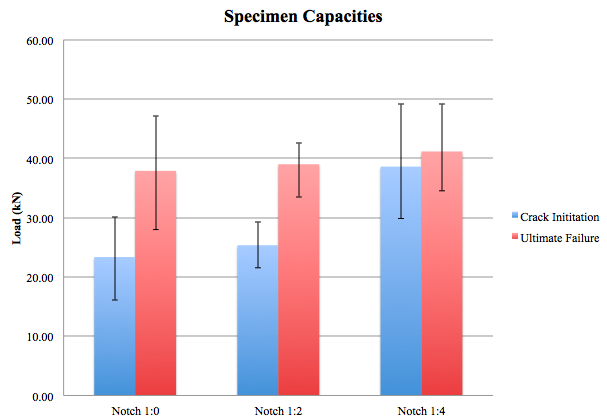
\includegraphics[scale=0.65]{Rect_Spec_Cap}}
	\end{center}
	\caption{Capacities for Rectangular Section Specimens}
	\label{fig:Rect_Spec_Cap}
\end{figure}

\noindent
The same trend is observed for the notch capacities, however there is a more dramatic increase between the average notch capacity of a 1:2 slope and a 1:4 slope; where the difference between a 1:0 and 1:2 slope notch capacity is 2kN and between a 1:2 and 1:4 slope is 13kN. There was a large amount of variance in the results, however this drastic increase between these notch capacities would support AS1720 and TMR's recommendation to use a 1:4 slope as it appears to improve the notch capacity tremendously. 

\vspace*{\baselineskip}

\noindent
The overall trend that can be observed in Figure \ref{tab:rect_Capac} proves the common theory that a notch which is chamfered will have a greater capacity than a rectangular end notch (slope 1:0), and thus the critical notch angle for a rectangular section beam is a 1:0 slope.

\vspace*{\baselineskip}

\noindent
Another relationship taken from the results in Table \ref{tab:rect_Capac} can be seen in Figure \ref{fig:Rect_Time}, which shows the time between the notch crack initiating and ultimate failure. The bars in Figure \ref{fig:Rect_Time} represent the average time interval for each notch slope and the error bars shows the variance in the results.  

\vspace*{\baselineskip}

\begin{figure}[h]
	\begin{center}
		\fbox{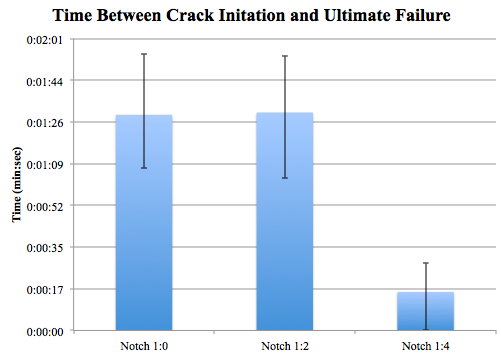
\includegraphics[scale=0.8]{Rect_Time}}
	\end{center}
	\caption{Time between notch initiating and ultimate failure for rectangular section specimens}
	\label{fig:Rect_Time}
\end{figure}

\noindent
From this graph, it can be seen that there is an increase of 1 second between the 1:0 slope and 1:2 slope notch. This slight increase in time may be indicative of an average pattern or may be due to the average water content in the 1:2 slope notch being greater than those in the 1:0 slope. Unfortunately this theory can be neither denied or confirmed due to the unknown water contents for the 1:0 slopes, thus the reason for this increase in time interval is ultimately unknown. The most interesting trend observed from Figure \ref{fig:Rect_Time} is that time average interval for the 1:4 slope notch is over a minute less than for the 1:0 slope and 1:2 slope, with an average of 16sec. This is not unexpected as it can be seen from Figure \ref{fig:Rect_Spec_Cap}, that by the time the notch crack initiates, the specimen is almost at ultimate capacity. However, when studying the results shown in Figure \ref{fig:Round-Crack-fail}, it becomes apparent that using a 1:4 chamfer notch may lead to notch failure occurring very close to or at the point of ultimate failure. From a maintenance perspective, this could be a major issue, as signs of notch cracking are hard to identify and are usually considered as means to observe the defect on a 1 to 6 monthly basis. As this experiment was conducted under short-term loading, it is hard to specify the time interval between crack initiation at the notch and ultimate failure for a long-term load. Nevertheless research into the effects of long-term loading on the time between crack initiation at the notch corner and ultimate failure is warranted. This will determine if notching cracking is a sign of ultimate failure for 1:4 notch slope, and possibly alter timber current maintenance schemes for timber bridges.


\subsubsection{Strain Gauge Analysis}
All strain gauge data shown in the following graphs start from an applied load of zero and end at the point of ultimate failure or when the strain gauge cut out, whichever came first. It should also be noted than the additional weight from loading plates and loading cell has been accounted. 

\vspace*{\baselineskip}

\noindent
\textbf{Notch Slope 1:0}\par
\noindent
Figure \ref{fig:Rect_10_def} shows the load-displacement graph from the LVDT results, for the rectangular section specimens, with a notch slope of 1:0. The trend in most of the specimens load vs deflection does not follow usual trends and is unexpected.
\begin{figure}[h]
	\begin{center}
		\fbox{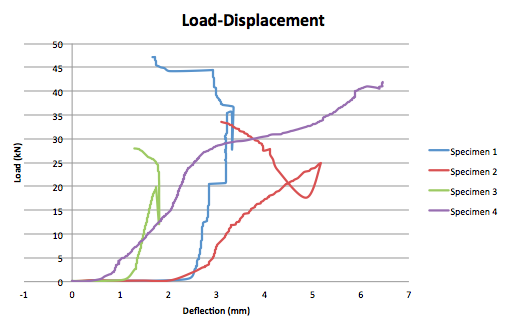
\includegraphics[scale=0.8]{Rect_10_Def}}
	\end{center}
	\caption{Load-Displacement Graph for Rectangular Beams with Notches of Slope 1:0}
	\label{fig:Rect_10_def}
\end{figure}

\pagebreak

\noindent
The load-displacement for specimen 1 is erratic and does not appear to have any distinct trend or any distinct correlation with either notch or ultimate failure load. For this reason, it is assumed that the LVDT results for specimen 1 are inaccurate, possible due to the plywood supporting the LVDT being too flimsy. As for specimens 2, the load-displacement graph follows the usual pattern, then ultimately changes direction at the point at which the notch crack initiates. The same pattern could be said for specimen 3, however it experiences more of a sudden drop which occurs after the notch crack initiates. This particular discrepancy is similar to that experienced in the loading chart, presumably due to the notch crack fully propagating through the specimen, and may be suggestive of this. Specimen 4's graph somewhat resembles a usual load-displacement curve, however after plateauing, begins to ascend again for no obvious reason and shows no discrepancies due to the notch failure.   

\begin{figure}[h]
	\begin{center}
		\fbox{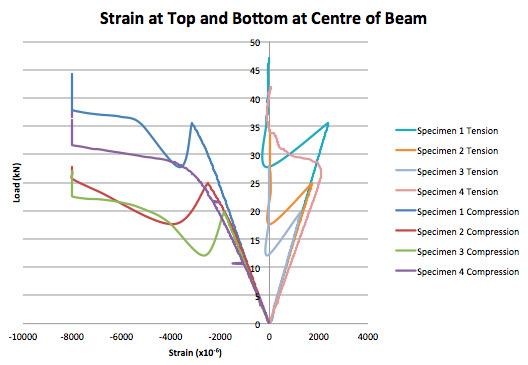
\includegraphics[scale=0.75]{Rect_10_Centre}}
	\end{center}
	\caption{Top and Bottom Strain at Centre for Rectangular Beams with Notches of Slope 1:0}
	\label{fig:Rect_10_centre}
\end{figure}

\pagebreak

\noindent
Figure \ref{fig:Rect_10_centre} shows the strains at the top (compressive) and bottom (tensile) of each specimen throughout loading. It can be seen for specimens 1, 2 and 3, that they follow the same trend where both tension and compression strains increase linearly to a spike in the data at the same load. After this, they both then experience a significant drop in load. This spike and sudden drop in load is suggestive of a sudden change in capacity and is assumed to be the point at which the notch crack fully propagates through the beam. Specimen 4 essentially followed the same trend, however there was no significant spike in the data, and instead experienced a smooth curve. This may be due to the notch crack in this particular specimen propagating more gradually than the other specimens. After the turning point for all specimens, the tensile strain eventuated to a strain of zero and the compressive strains continue increasing to a strain of roughly --8000 $\times 10^{-6}$, where it suddenly stopped increasing in strain and only increased in load until ultimate failure.  

\begin{figure}[h]
	\begin{center}
		\fbox{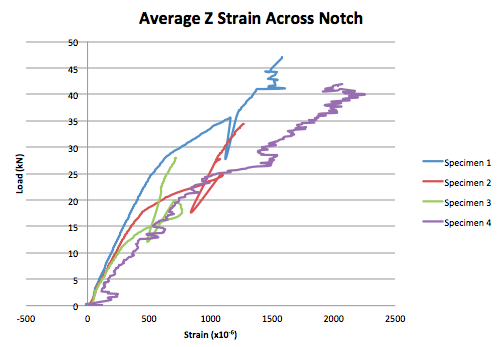
\includegraphics[scale=0.8]{Rect_10_Z}}
	\end{center}
	\caption{Horizontal Strain at Centre for Rectangular Beams with Notches of Slope 1:0}
	\label{fig:Rect_10_Z}
\end{figure}
\pagebreak

\noindent
The average horizontal strain at the notch corner can be seen in Figure \ref{fig:Rect_10_Z}, where the horizontal strain were collected from either side of the notch and averaged across the section. From the graph, it can be seen that specimens 1, 2 and 3 experience similar trends in horizontal strain, where they increase and then suddenly drop at the same load at which the compressive and tensile strains dropped. Specimen 4, on the other hand is very erratic, and is hard to identify a definite trend. However, this erratic graph may be indicative of a slow growing notch crack.

\vspace*{\baselineskip}

\noindent
The vertical strains were also average across the both sides of the notch, as shown in Figure \ref{fig:Rect_10_Y}. From this graph, a pattern can be seen for specimens 1 and 3, where there is a large spike in the Y strain at a load, after which the strain dramatically drops to below zero. The load at which this data drops aligns with the load at which the notch crack initiates. Specimen 4's data somewhat follows to same trend, but is again erratic, so a definite trend is unable to be established. 

\begin{figure}[h]
	\begin{center}
		\fbox{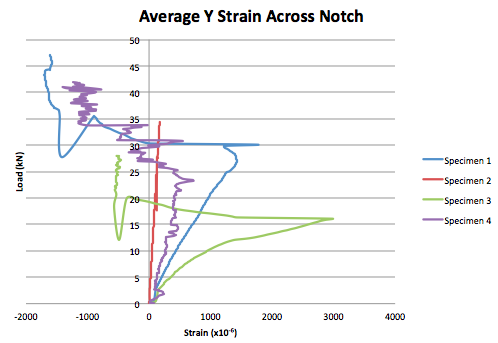
\includegraphics[scale=0.8]{Rect_10_Y}}
	\end{center}
	\caption{Vertical Strain at Centre for Rectangular Beams with Notches of Slope 1:0}
	\label{fig:Rect_10_Y}
\end{figure}
\pagebreak

\noindent
The data for specimen 1 does not follow the same trend and appears to be constantly increasing until ultimate failure. There is a small discrepancy in the data around the load at which the notch corner crack initiated, however the point at which this occurs is not easily defined. Overall, the vertical strain in specimen 2 appears to be inaccurate as it does not follow a similar trend observed in the other specimens. A possible reason this data may be inaccurate is due to a large wedge cut out of the notched end of the beam, as shown in Figure \ref{fig:Rect_2_wedge}, which may have been in line with the strain gauge and obscuring the data. 
\vspace*{\baselineskip}

\begin{figure}[h]
	\begin{center}
		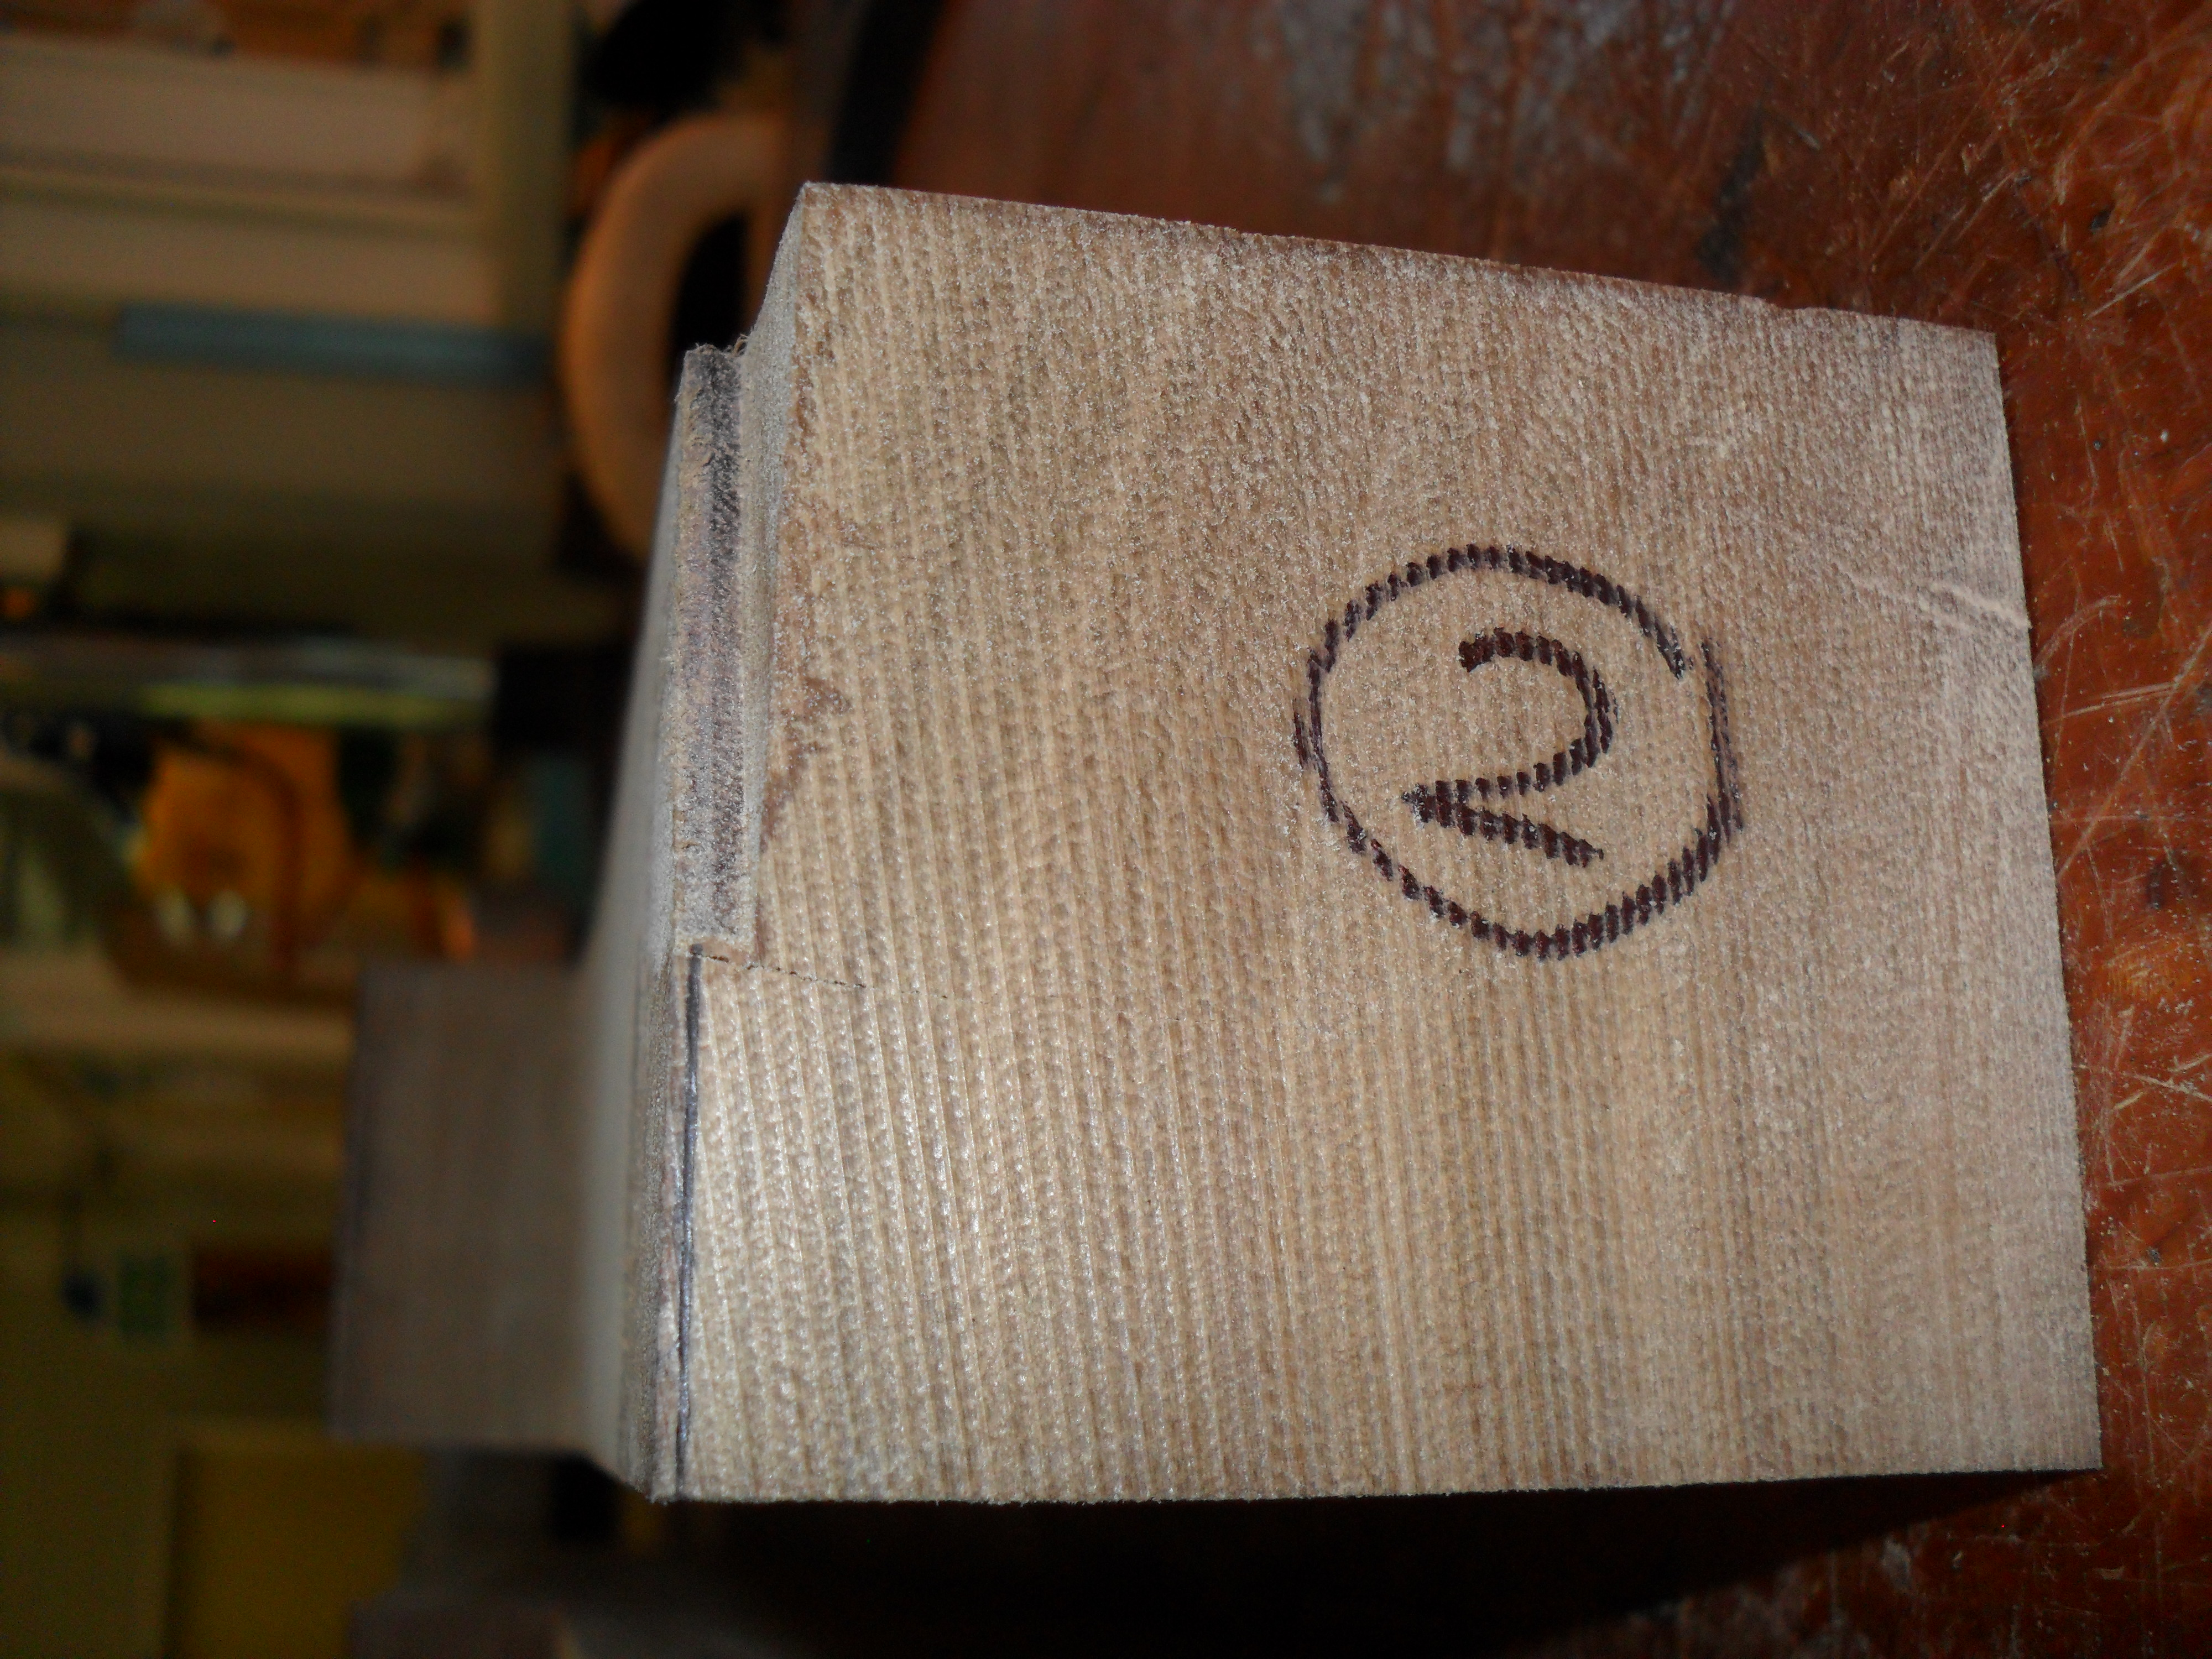
\includegraphics[scale=0.065]{End_wedge}
		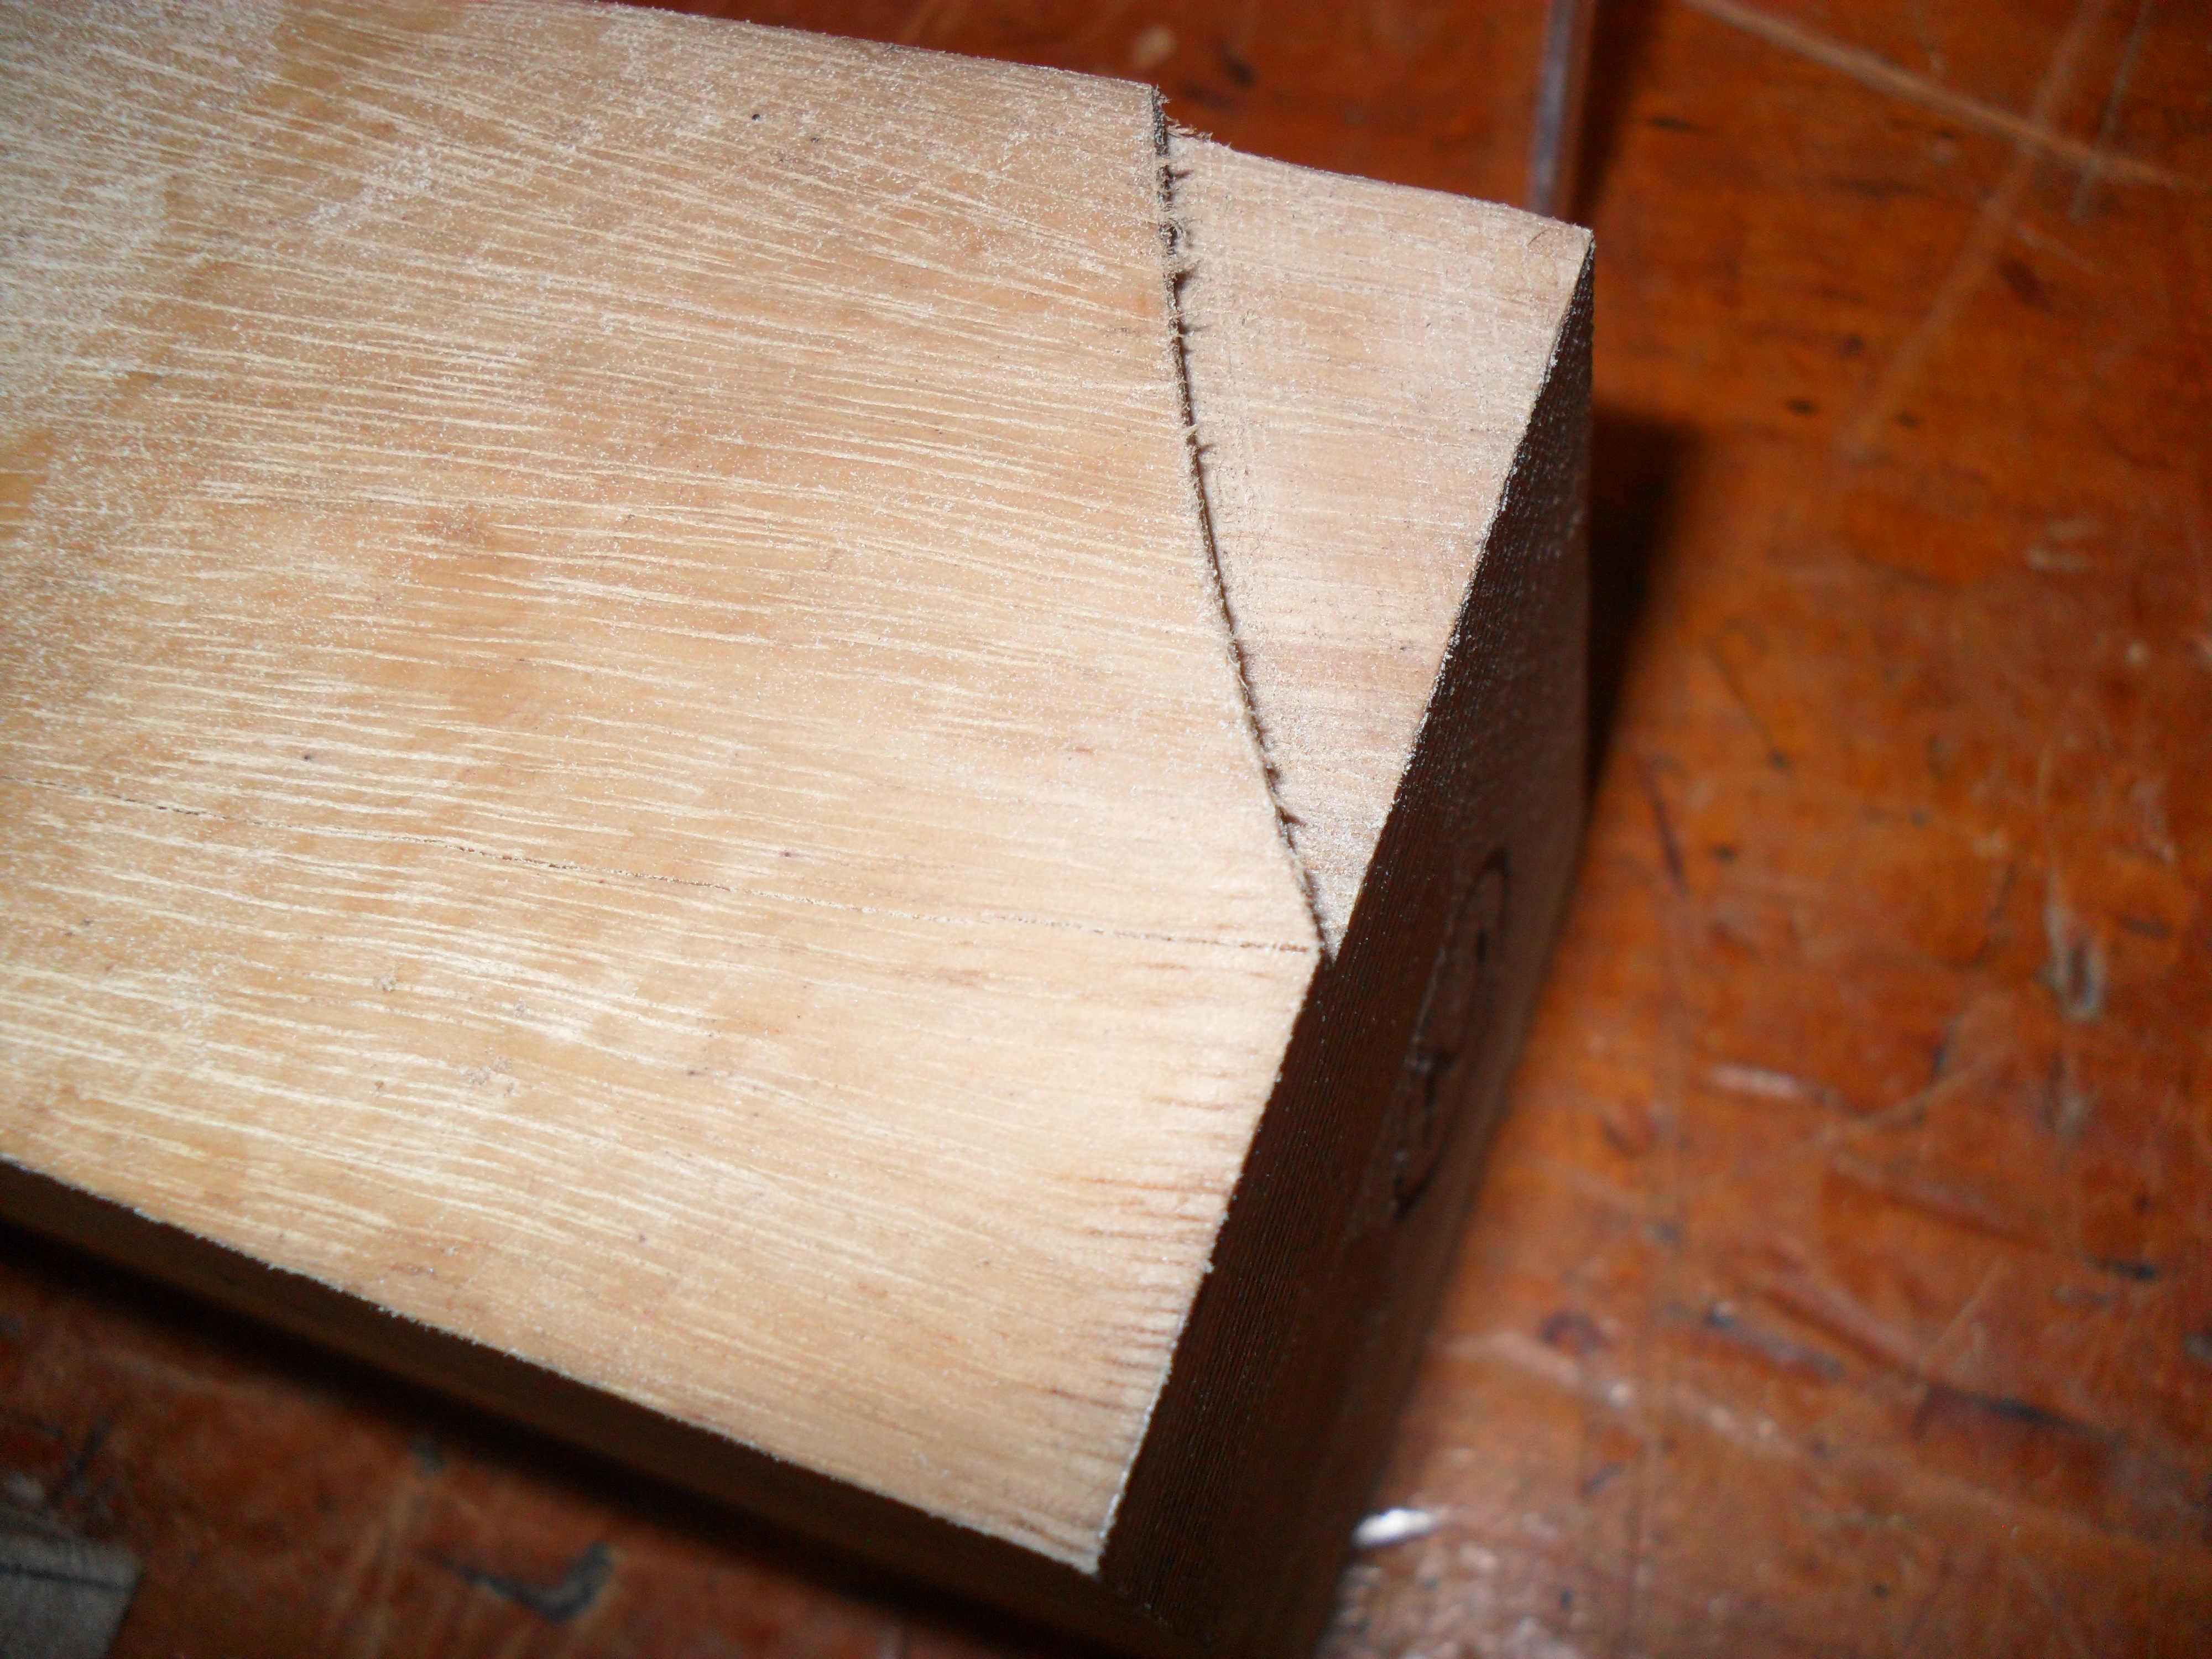
\includegraphics[scale=0.065]{Top_wedge}
	\end{center}
	\caption{Rectangular specimen 2 notch slope 1:0; wedge defect}
	\label{fig:Rect_2_wedge}
\end{figure}

\pagebreak

\noindent
\textbf{Notch Slope 1:2}\par
\noindent

\begin{figure}[h]
	\begin{center}
		\fbox{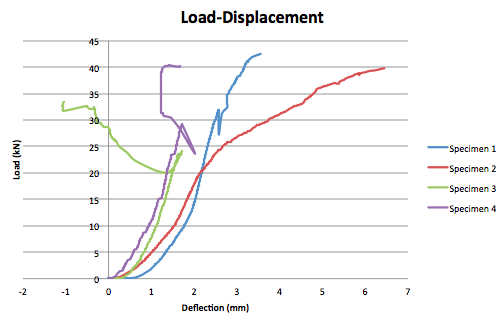
\includegraphics[scale=0.8]{Rect_12_Def}}
	\end{center}
	\caption{Load-Displacement Graph for Rectangular Beams with Notches of Slope 1:2}
	\label{fig:Rect_12_def}
\end{figure}


\begin{figure}[h]
	\begin{center}
		\fbox{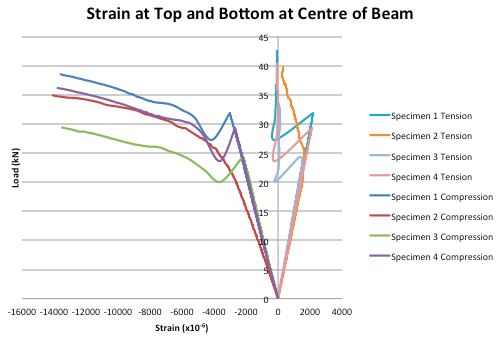
\includegraphics[scale=0.75]{Rect_12_Centre}}
	\end{center}
	\caption{Top and Bottom Strain at Centre for Rectangular Beams with Notches of Slope 1:2}
	\label{fig:Rect_12_centre}
\end{figure}

\begin{figure}[h]
	\begin{center}
		\fbox{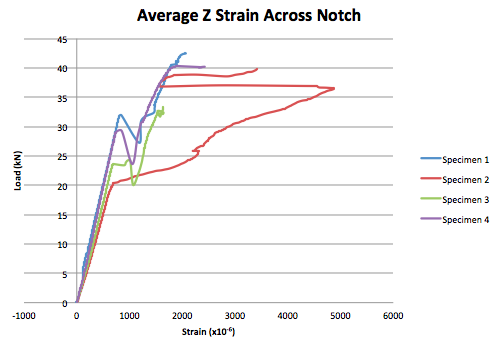
\includegraphics[scale=0.8]{Rect_12_Z}}
	\end{center}
	\caption{Horizontal Strain at Centre for Rectangular Beams with Notches of Slope 1:2}
	\label{fig:Rect_12_Z}
\end{figure}

\begin{figure}[h]
	\begin{center}
		\includegraphics[scale=0.065]{Cut_Top}
		\includegraphics[scale=0.065]{Cut_Side}
	\end{center}
	\caption{Rectangular specimen 2 notch slope 1:2; thick cut defect}
	\label{fig:Rect_Cut}
\end{figure}

\begin{figure}[h]
	\begin{center}
		\fbox{\includegraphics[scale=0.8]{Rect_12_Y}}
	\end{center}
	\caption{Vertical Strain at Centre for Rectangular Beams with Notches of Slope 1:2}
	\label{fig:Rect_12_Y}
\end{figure}

\vspace*{\baselineskip}

\noindent
\textbf{Notch Slope 1:4}\par
\noindent

\vspace*{\baselineskip}
\noindent Discuss variance in results relating to water contents and existing defects \par

\subsection{Round Specimens}
\subsubsection{Failure Modes}
\vspace*{\baselineskip}
\noindent Compiled graphs showing exact data from results for load displacement, centre tension, centre compression, z-stress and y-stress \par

\vspace*{\baselineskip}

\pagebreak
\captionof{table}{Round Specimen Water Contents and Initial Failure Locations}
\begin{center}
	\begin{tabular}{|c|c|c|p{4.5cm}|} 
		\hline
		
		\textbf{Notch Angle Slope} & \textbf{Specimen No.} & \textbf{Water Content (\%)} & \textbf{Location of Initial Failure}\\ [0.5ex]
		\hline
		
		1:0 & 1 & 22 & Cracked propagated from existing crack at opposite end, then cracked at notch corner  \\ [0.5ex]
		\hline
		1:0 & 2 & 21 & Cracked at notch corner  \\ [0.5ex]
		\hline
		1:0 & 3 & 24 & Cracked at notch corner  \\ [0.5ex]
		\hline
		1:0 & 4 & 26 & Cracked at notch corner \\ [0.5ex]
		\hline
		
		1:2 & 1 & 23 & Cracked at notch corner \\ [0.5ex]
		\hline
		1:2 & 2 & 30 & Cracked at notch corner \\ [0.5ex]
		\hline
		1:2 & 3 & 22 & Cracked at notch corner \\ [0.5ex]
		\hline
		1:2 & 4 & 29 & Cracked at notch corner \\ [0.5ex]
		\hline
		
		1:4 & 1 & 24 & Cracked at notch corner \\ [0.5ex]
		\hline
		1:4 & 2 & 22 & Cracked propagated half way down chamfer, then cracked at notch corner \\ [0.5ex]
		\hline
		1:4 & 3 & 27 & Cracked at notch corner \\ [0.5ex]
		\hline
		1:4 & 4 & 23 & Full member failed (notch didn't fail) \\ [0.5ex]
		\hline
		
	\end{tabular}
\end{center}


\vspace*{\baselineskip}
\noindent Table showing cracking and ultimate loads and times \par

\captionof{table}{Round Specimen Crack Inititation and Ultimate Loads}
\begin{center}
	\begin{tabularx}{\textwidth}{|>{\centering}X|>{\centering}X|>{\centering}X|>{\centering}X|>{\centering}X|>{\centering}X|} 
		\hline
		
		\textbf{Notch Angle Slope} & \textbf{Specimen No.} & \textbf{Notch Crack Initiation (kN)} & \textbf{Time for Notch to Crack (min:sec)} & \textbf{Ultimate Failure (kN)} & \textbf{Time to Ultimate Failure (min:sec)} \tabularnewline [0.5ex] 
		\hline
		1:0 & 1 & 53.50 & 05:20 & 59.98 & 06:00 \tabularnewline [0.5ex]
		\hline
		1:0 & 2 & 44.46 & 04:25 & 60.06 & 05:59 \tabularnewline [0.5ex]
		\hline
		1:0 & 3 & 36.23 & 03:49 & 55.91 & 05:55 \tabularnewline [0.5ex]
		\hline
		1:0 & 4 & 22.76 & 02:15 & 36.62 & 03:38 \tabularnewline [0.5ex]
		\hline
		
		1:2 & 1 & 47.68 & 03:48 & 61.83 & 04:57 \tabularnewline [0.5ex]
		\hline
		1:2 & 2 & 47.05 & 04:41 & 53.42 & 05:19 \tabularnewline [0.5ex]
		\hline
		1:2 & 3 & 64.65 & 06:26 & 76.94 & 07:40 \tabularnewline [0.5ex]
		\hline
		1:2 & 4 & 38.92 & 03:50 & 42.99 & 04:18 \tabularnewline [0.5ex]
		\hline
		
		1:4 & 1 & 47.56 & 04:45 & 49.11 & 04:50 \tabularnewline [0.5ex]
		\hline
		1:4 & 2 & 58.48 & 05:46 & 58.48 & 05:46 \tabularnewline [0.5ex]
		\hline
		1:4 & 3 & 65.76 & 06:50 & 70.69 & 07:03 \tabularnewline [0.5ex]
		\hline
		1:4 & 4 & N/A & N/A & 69.01 & 06:52 \tabularnewline [0.5ex]
		\hline
		
	\end{tabularx}
\end{center}

\subsubsection{Loading Rates}
The loading rates used for the round specimens can be seen in Figure \ref{fig:Round_load}. The load rate was constantly 10kN per minute for all specimens, except for specimens 1 for notch slopes 1:0 and 1:4, which experienced a load rate of 8kN per minute. This error in loading rate was due to an error in the MTS loading settings which was fixed for the rest of the experiments.

\begin{figure}[h]
	\begin{center}
		\fbox{\includegraphics[scale=0.7]{Round_load}}
	\end{center}
	\caption{Load rates for round specimens}
	\label{fig:Round_load}
\end{figure}

\noindent
The same extreme drop in load occurred in most of the round specimens as did in the rectangular specimens, however were less prominent (i.e. less of a decrease) than those present in Figure \ref{fig:Rect_load}. Another difference between the round and rectangular specimen loading graphs were that some of the round specimens did not experience an extreme decrease in load. As it was presumed for the rectangular specimens that the decrease was due the notch fully propagating, it would be safe to assume the same for the round specimens, where the ones that didn't experience a drop, did not crack at the notch corner. 

\vspace*{\baselineskip}

\noindent
It should also be noted that specimen 1 of notch slope 1:2 was unable to be plotted on this graph as the load cell malfunctioned during the loading and the load was then taken from the MTS. The load data collected from the MTS machine was taken at slightly different load points than the data taken using the data logger, thus the loads and times were unable to be exactly aligned. However, the MTS was set to load this specimen at a rate of 10kN per minute.  


\subsubsection{Strain Gauge Analysis}
Due to the curvature of the specimens, the strain gauges experienced some initial strain before loading began. To account for this, the strain gauges were zeroed before loading commenced (i.e.at a load of zero).

\subsection{Predicted Capacities using Standards}

\vspace*{\baselineskip}
\noindent Tables with predicted capacities from AS1720, Eurocode 5 and CSA O.86\par


\vspace*{\baselineskip}
\noindent Trends in rectangular and round specimen results (noting the critical angle, failure modes and time between crack initiation and ultimate failure) \par

\vspace*{\baselineskip}

\noindent
Figure \ref{fig:Round-Crack-fail} shows the time between the crack initiating at the notch corner and ultimate failure for the round specimens. The blue bar in the graph indicates the average time and the error bars shows the variance in the results. 

	\begin{figure}[h]
		\begin{center}
		\fbox{\includegraphics[scale=0.8]{Round_crack_fail}}
		\end{center}
		\caption{Time between notch crack initiation and ultimate failure}
		\label{fig:Round-Crack-fail}
	\end{figure}

From this graph, a trend can be observed, where the time between the notch cracking and ultimate failure significantly decreases with an increasing notch slope. This was not unexpected, as it appears from previous results that the increase in notch slope increases the capacity of the notch, thus the load at which the notch cracks is getting closer to the ultimate capacity of the beam. 

\vspace*{\baselineskip}
\noindent Discuss/determine a relationship between rectangular and round specimens\par

\vspace*{\baselineskip}
\noindent Look into round design and apply the new As for the notched end to see results and maybe discuss a factor for a notched member\par

\vspace*{\baselineskip}
\noindent Include and discuss graphs comparing the results to predicted capacities from Australian Standards, Eurocode 5 and CSA O.86. Discuss which design yields the best results and why. \par

\vspace*{\baselineskip}
\noindent Compare actual strain/stress results with ANSYS results at the untimate failure load\par

\pagebreak	

\subsection{Finite Element Analysis}
\noindent
A small scale ANSYS model has also been established to determine the optimum placement for data reading equipment and critical loading set-out for all tests. Figures \ref{fig:Def} to \ref{fig:fig:y_norm} show the ANSYS analysis for the rectangular end notched specimen, centrally loaded and simply supported.

\vspace*{\baselineskip}

\begin{figure}[h]
	\begin{center}
		\includegraphics[scale=0.45]{Ansys_Deflection}
	\end{center}
	
	\caption{Rectangular Section Beam: Deflection}
	\label{fig:Def}
\end{figure}
\pagebreak

\begin{figure}[h]
	\begin{center}
		\includegraphics[scale=0.45]{YZ_shear_strain}
	\end{center}
	\caption{Rectangular Section Beam: XY-Plane Shear Strain}
	\label{fig:yz_shear}
\end{figure}

\begin{figure}[h]
	\begin{center}
		\includegraphics[scale=0.45]{y_normal_strain}
		\includegraphics[scale=0.45]{z_normal_strain}
	\end{center}
	\caption{Rectangular Section Beam: Normal Strain in Y-direction (upper) and Z-direction (lower)}
	\label{fig:fig:y_norm}
\end{figure}
\pagebreak

\section{Conclusions}
\vspace*{\baselineskip}
\noindent Concluded which was the critical angle, most common failure modes and time between crack initiation and ultimate failure for both rectangular and round specimens\par

\vspace*{\baselineskip}
\noindent Was a relationship between rectangular and round specimens determined? What was it/why not?\par

\vspace*{\baselineskip}
\noindent Which code yielded the best results\par

\vspace*{\baselineskip}
\noindent Was the finite element analysis accurate in comparison to actual results?\par

\pagebreak	

\bibliographystyle{unsrt}
\bibliography{My_Library.bib}

\pagebreak
\cleardoublepage
\pagenumbering{gobble}

\appendixtitleon

\begin{appendices}
	\section{\textit{Rectangular Specimen Characteristics}}
\pagebreak

\end{appendices}

\begin{appendices}
	\section{\textit{Round Specimen Characteristics}}
	\pagebreak
	
\end{appendices}

\end{document}
